\chapter{二维离散Cat映射的状态网络分析}

\section{二维离散Cat映射的定义}

Arnold's Cat映射$f(x, y)=(x+y, x+2y)\pmod 1$是最著名的混沌映射之一,它在有限区域内进行反复折叠、拉伸变化,可用来置换图像像素的位置
\cite[Fig. 1.17]{arnol1968mathematical},
其矩阵表示形式为
\begin{equation}
f(\textbf{x})=(\Phi \cdot \textbf{x})\pmod N,
\label{eq:ArnoldMatrix}
\end{equation}
其中$N$为正整数,$\textbf{x}$为$n\times 1$向量,$\Phi$为$n\times n$矩阵,且其行列式为1。
Cat映射可以通过各种方法进行扩展,如改变变换矩阵$\Phi$的元素范围\upcite{Chen:CSF:2004};
将变换矩阵扩展到2维,3维甚至更高维\upcite{kwok2007generalCatMap};修改模数$N$\upcite{Wu:catmapITC:2016}。

二维有限整数域上的扩展离散Cat映射(GDCM)在密码学领域有着十分广泛的应用,例如其可以直接应用于图像像素位置置乱,
其矩阵表示形式为
\begin{equation}
f
\begin{bmatrix}
		x_{n} \\
		y_{n}
	\end{bmatrix}=
	\begin{bmatrix}
		x_{n+1} \\
		y_{n+1}
	\end{bmatrix}
	=
	\begin{bmatrix}
		1 & p    \\
		q & 1+p\cdot q
	\end{bmatrix}\cdot
	\begin{bmatrix}
		x_{n} \\
		y_{n}
	\end{bmatrix}
	\bmod N,
	\label{eq:ArnoldInteger}
\end{equation}
这里$x_n, y_n\in \mathbb{Z}_N$,$p, q, N\in \mathbb{Z}^+$。

\begin{figure*}[!htb]
\centering
\begin{minipage}{0.45\FourImW}
\centering\hfill
\raisebox{0.25\FourImW}{
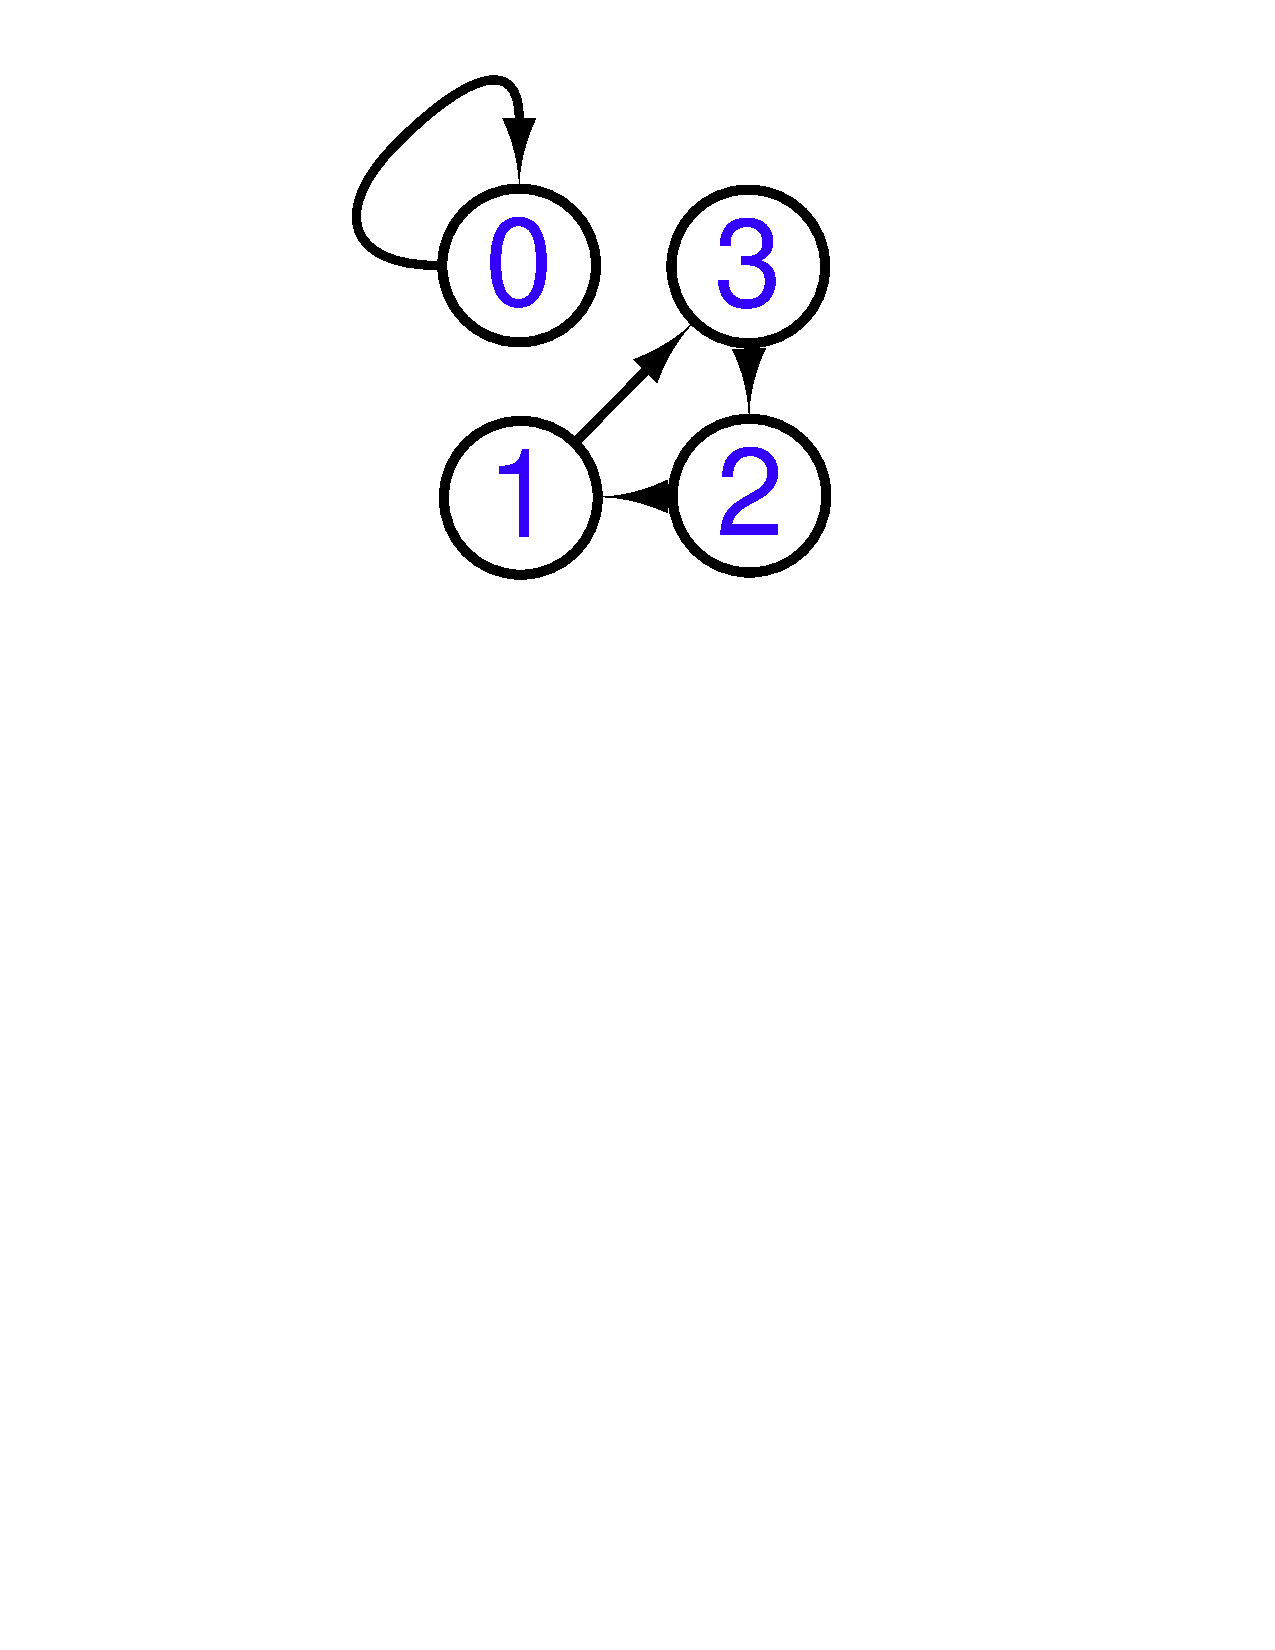
\includegraphics[width=0.45\FourImW]{a1_b1_e1}}
a)
\end{minipage}\hspace{6em}
\begin{minipage}{0.85\FourImW}
\centering
\raisebox{0.15\FourImW}{\hfill
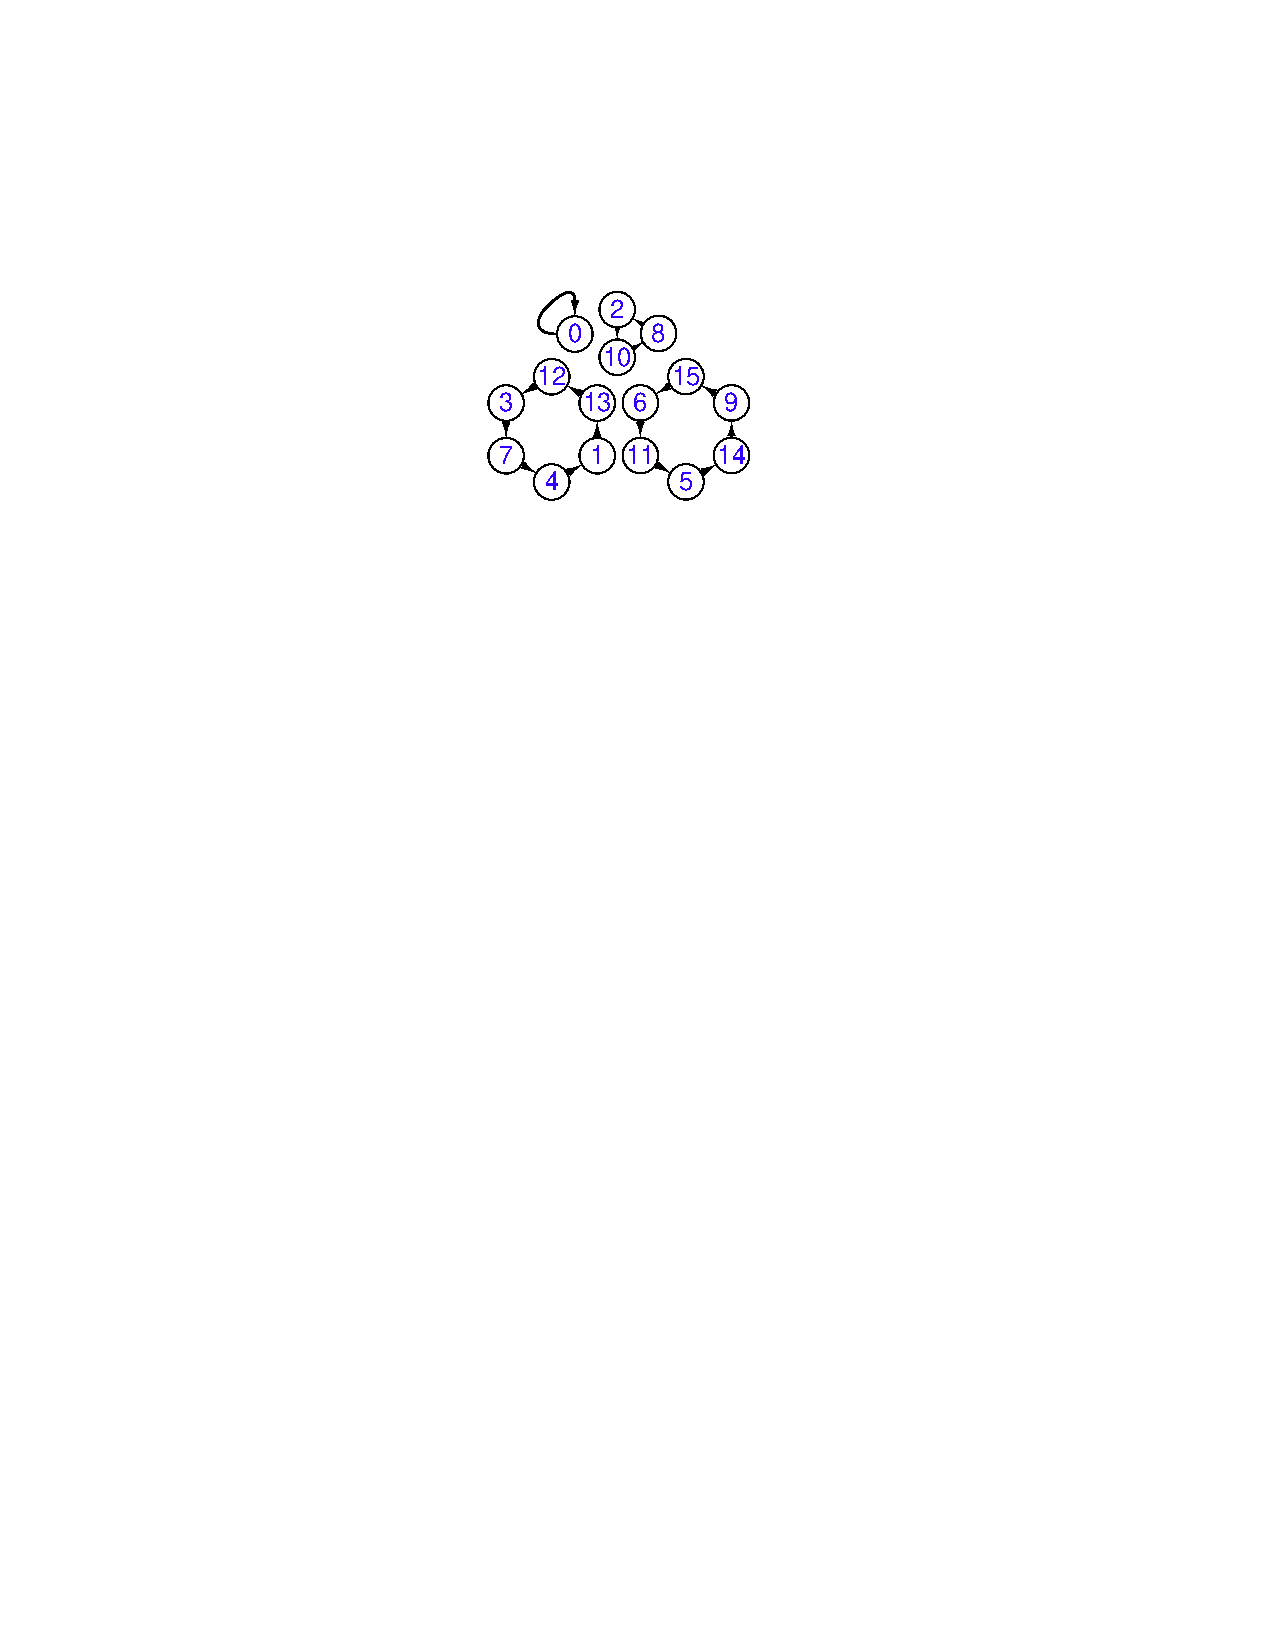
\includegraphics[width=0.85\FourImW]{a1_b3_e2}}
b)
\end{minipage} \hspace{6em}
\begin{minipage}{1.25\FourImW}
\centering
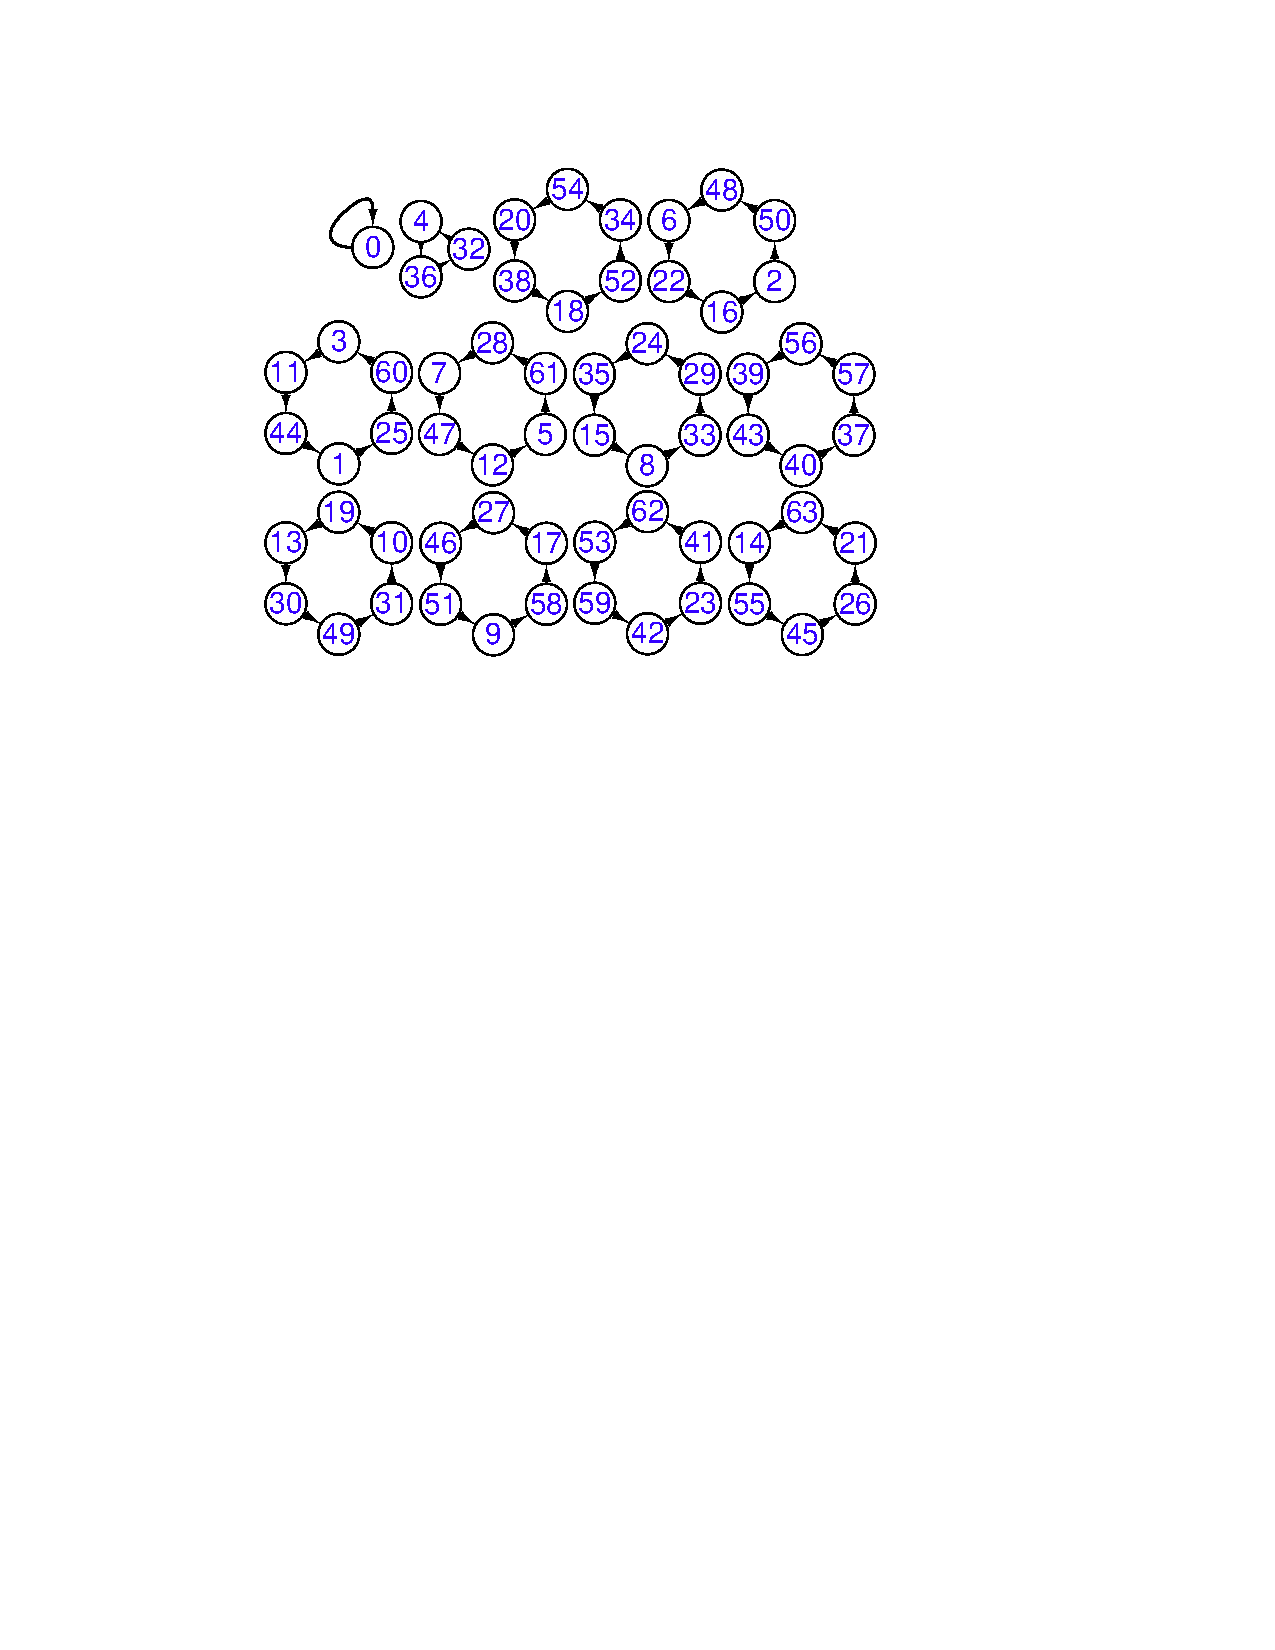
\includegraphics[width=1.25\FourImW]{a1_b3_e3}
c)
\end{minipage}\hspace{\figsep}
\begin{minipage}{2\BigOneImW}
\centering
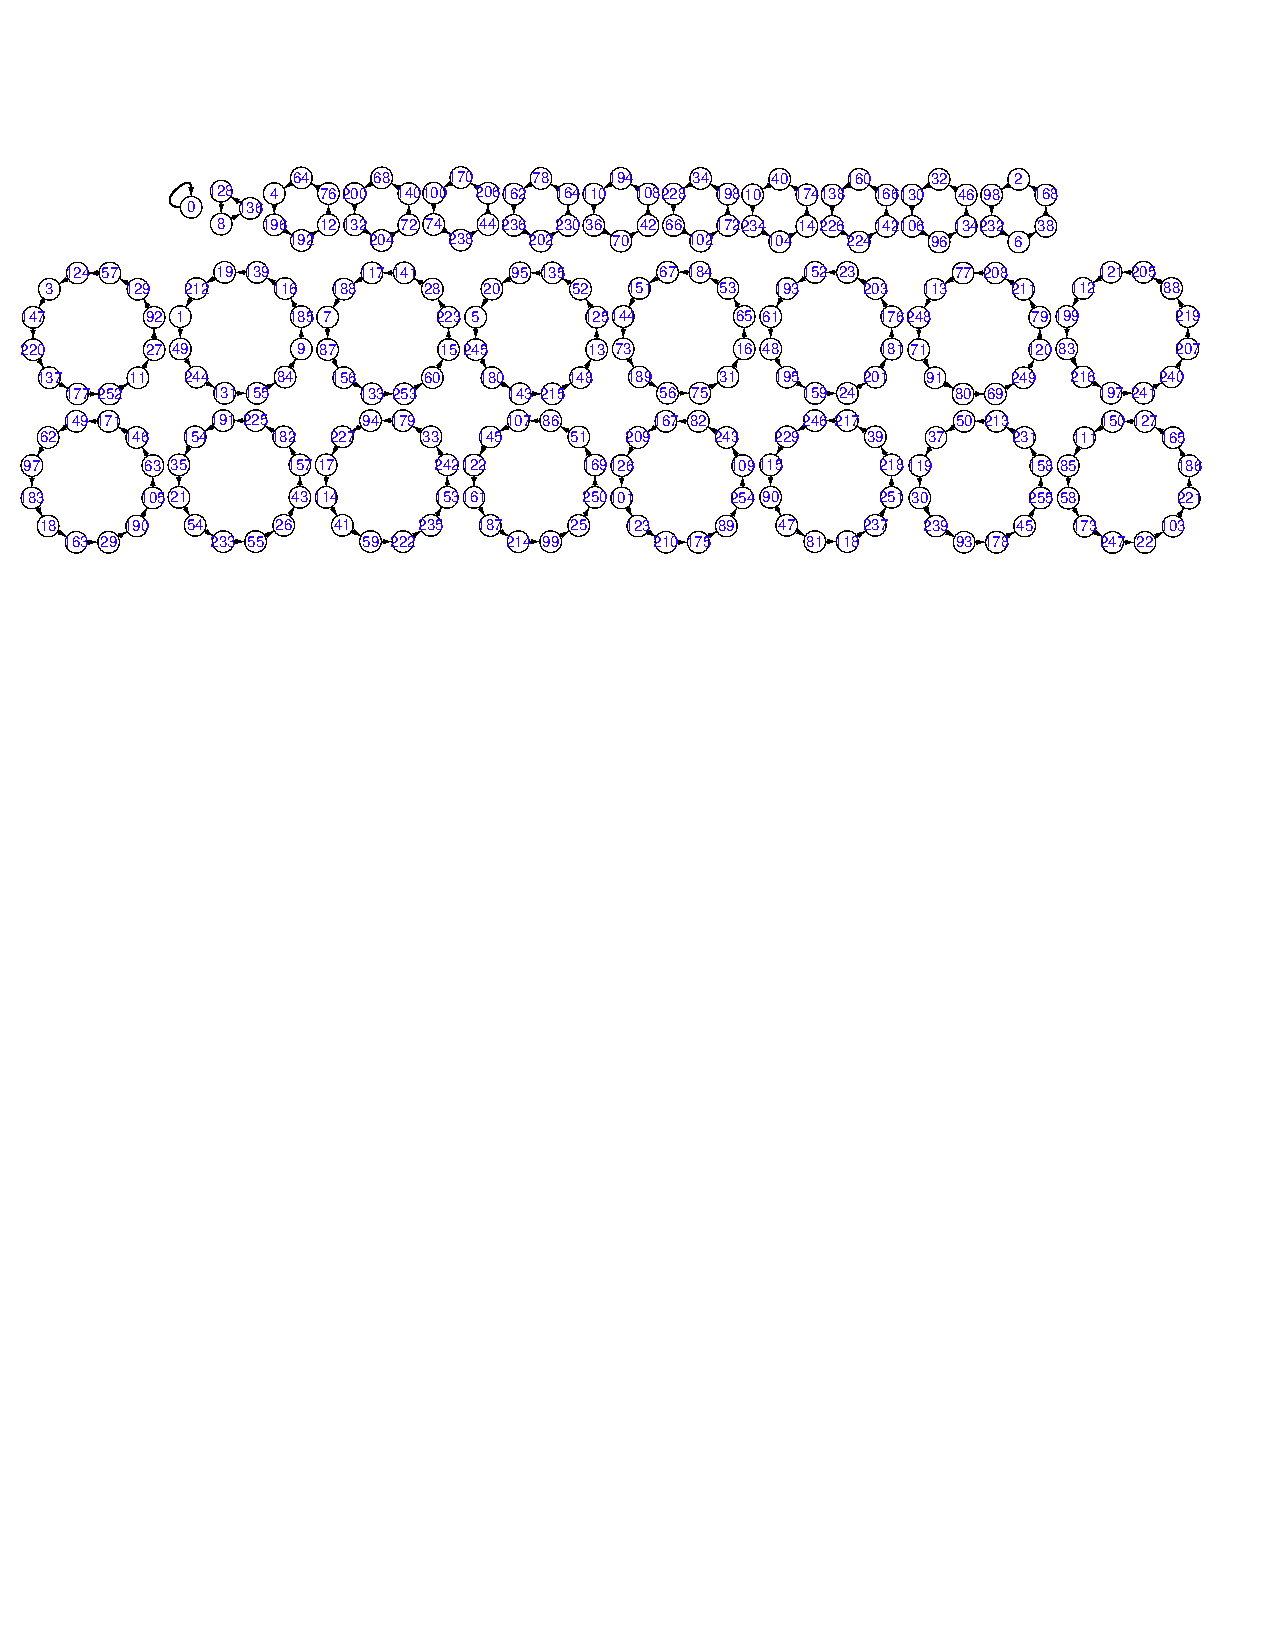
\includegraphics[width=2\BigOneImW]{a1_b3_e4}
d)
\end{minipage}
\caption{有限域$\mathbb{Z}_{2^e}$上GDCM~(\ref{eq:ArnoldInteger})的状态映射网络,其中$(p, q)=(1, 3)$:
a) $e=1$; b) $e=2$; c) $e=3$; d) $e=4$}
\label{fig:SMNcat}
\end{figure*}

1992年,Dyson等人从理论上推导出了控制参数$(p, q)=(1, 1)$时GDCM~(\ref{eq:ArnoldInteger})的周期上界和下界\upcite{dyson1992periodCat};
2012年,J. Bao等人进一步揭示了某些约束条件下GDCM~(\ref{eq:ArnoldInteger})的相关性质\upcite{Bao:ND:2012};
在\upcite{chen2012periodpe,Chen:linearCNSNS:2012,Catchen2013period2e,chen2014period:TCS14}中,
F. Chen使用Hensel上升法准确推导出了任意参数$p,q$下GDCM~(\ref{eq:ArnoldInteger})的周期分布,
整个分析根据$N$对$(\mathbb{Z}_{N}, +, \cdot)$的代数性质的影响分为三部分:
N为素数时$(\mathbb{Z}_{N}, +, \cdot)$为伽罗瓦域\upcite{Chen:linearCNSNS:2012};
N为素数的幂时$(\mathbb{Z}_{N}, +, \cdot)$为伽罗瓦环\upcite{chen2012periodpe,Catchen2013period2e};
N为常见复合数时$(\mathbb{Z}_{N}, +, \cdot)$为交换环\upcite{chen2014period:TCS14}。
根据所用分析方法,第二种情况又分为两种子情况$N=p^e$和$N=2^e$,其中$p$为大于等于3的素数,e为整数。
从数字设备中实际应用的角度来看,Galois环的情况最为重要,因为它与$e$比特定点运算格式表示的数字集同构。

\section{定点域上离散Cat映射的性质分析}

\begin{Property}
$T$的表示形式由$p$和$q$的奇偶性决定:
\begin{equation}
  T=
  \left.\begin{cases}
  2^k,           & 2\mid p \mbox{ 或~} 2\mid q;\\
  3\cdot 2^{k'}, & 2\nmid p \mbox{ 且~} 2\nmid q.
  \end{cases}\right.
  \label{eq:T}
\end{equation}
其中$k\in \{0, 1, \cdots, e\}$,$k'\in \{0, 1, \cdots, e-2\}$。
\label{prop:period}
\end{Property}

GDCM~(\ref{eq:ArnoldInteger})的周期$T$的表示形式如~(\ref{eq:T})式所示,这里$N=2^e$。
周期为$T$的不同Cat映射的数量$N_T$与周期$T$之间的关系被准确推导:
\begin{eqnarray}
N_T=
\begin{cases}
1                         & T=1;  \\
3                         & T=2;  \\	
2^{e+1}+12                & T=4;  \\
2^{e-1}+2^{e}             & T=6;  \\
2^{e+k-2}+3\cdot 2^{2k-2} & T=2^k,\ k\in \{3, 4, \cdots, e-1\};\\
2^{2e-2}                  & T=2^e; \\
2^{e+k-1}                 & T=3\cdot 2^k, k\in \{0, 2, 3, \cdots, e-2\},
\end{cases}
\label{eq:numberMaps}
\end{eqnarray}
其中$e\ge 4$。

当$e=3$时,
\begin{eqnarray*}
N_T=\begin{cases}
	1              & T=1;  \\
	3              & T=2;  \\	
    2^{e-1}        & T=3;  \\	
	2^{e+1}+12     & T=4;  \\
	2^{e-1}+2^{e}  & T=6;  \\		
	2^{2e-2}       & T=8,
\end{cases}
\end{eqnarray*}
不可以表示为表\cite[Table III]{Catchen2013period2e}所示一般形式(\ref{eq:numberMaps}),例如当$e=k=3$时,
$2^{2e-2}\neq 2^{e+k-2}+3\cdot 2^{2k-2}$。根据~(\ref{eq:numberMaps})式可知:当$T\le 6$时,GDCM
~(\ref{eq:ArnoldInteger})的数量$N_T=(1+3+2^{e-1}+2^{e+1}+12+2^{e-1}+2^{e})=2^{e+2}+16$。
$e\ge 32$时,这对普通数字计算机来说是一个巨大的数字。

GDCM~(\ref{eq:ArnoldInteger})对应的状态映射网络$F_e$可通过以下方式构造:
$1)$将$N^2$个可能状态看作$N^2$个节点;$2)$若$\textbf{x}_2=f(\textbf{x}_1)$,则对应向量$\textbf{x}_1=(x_1, y_1)$的节点
指向对应向量$\textbf{x}_2=(x_2, y_2)$的节点。为方便起见,采用双射$z_n=x_{n} + (y_{n} \cdot N)$对GDCM~(\ref{eq:ArnoldInteger})
的二维向量进行降维处理。为进一步阐明GDCM~(\ref{eq:ArnoldInteger})的状态映射网络关于定点运算精度$e$的变化,令
\begin{equation}
z_{n, e} = x_{n, e} + (y_{n, e} \cdot 2^e),
\label{eq:quantization}
\end{equation}
其中$x_{n, e}, y_{n, e}$分别表示$N=2^e$时GDCM~(\ref{eq:ArnoldInteger})的向量分量$x_{n}, y_{n}$。
图~\ref{fig:SMNcat}为$(p, q)=(1, 3)$时有限域上GDCM~(\ref{eq:ArnoldInteger})的状态映射网络$F_e$。
根据图~\ref{fig:SMNcat}可以看出,GDCM~(\ref{eq:ArnoldInteger})的状态映射网络随着定点运算精度$e$的增大呈现出很强的规律性。

\begin{figure}[!htb]
	\centering
	\begin{minipage}{0.77\FourImW}
		\centering
		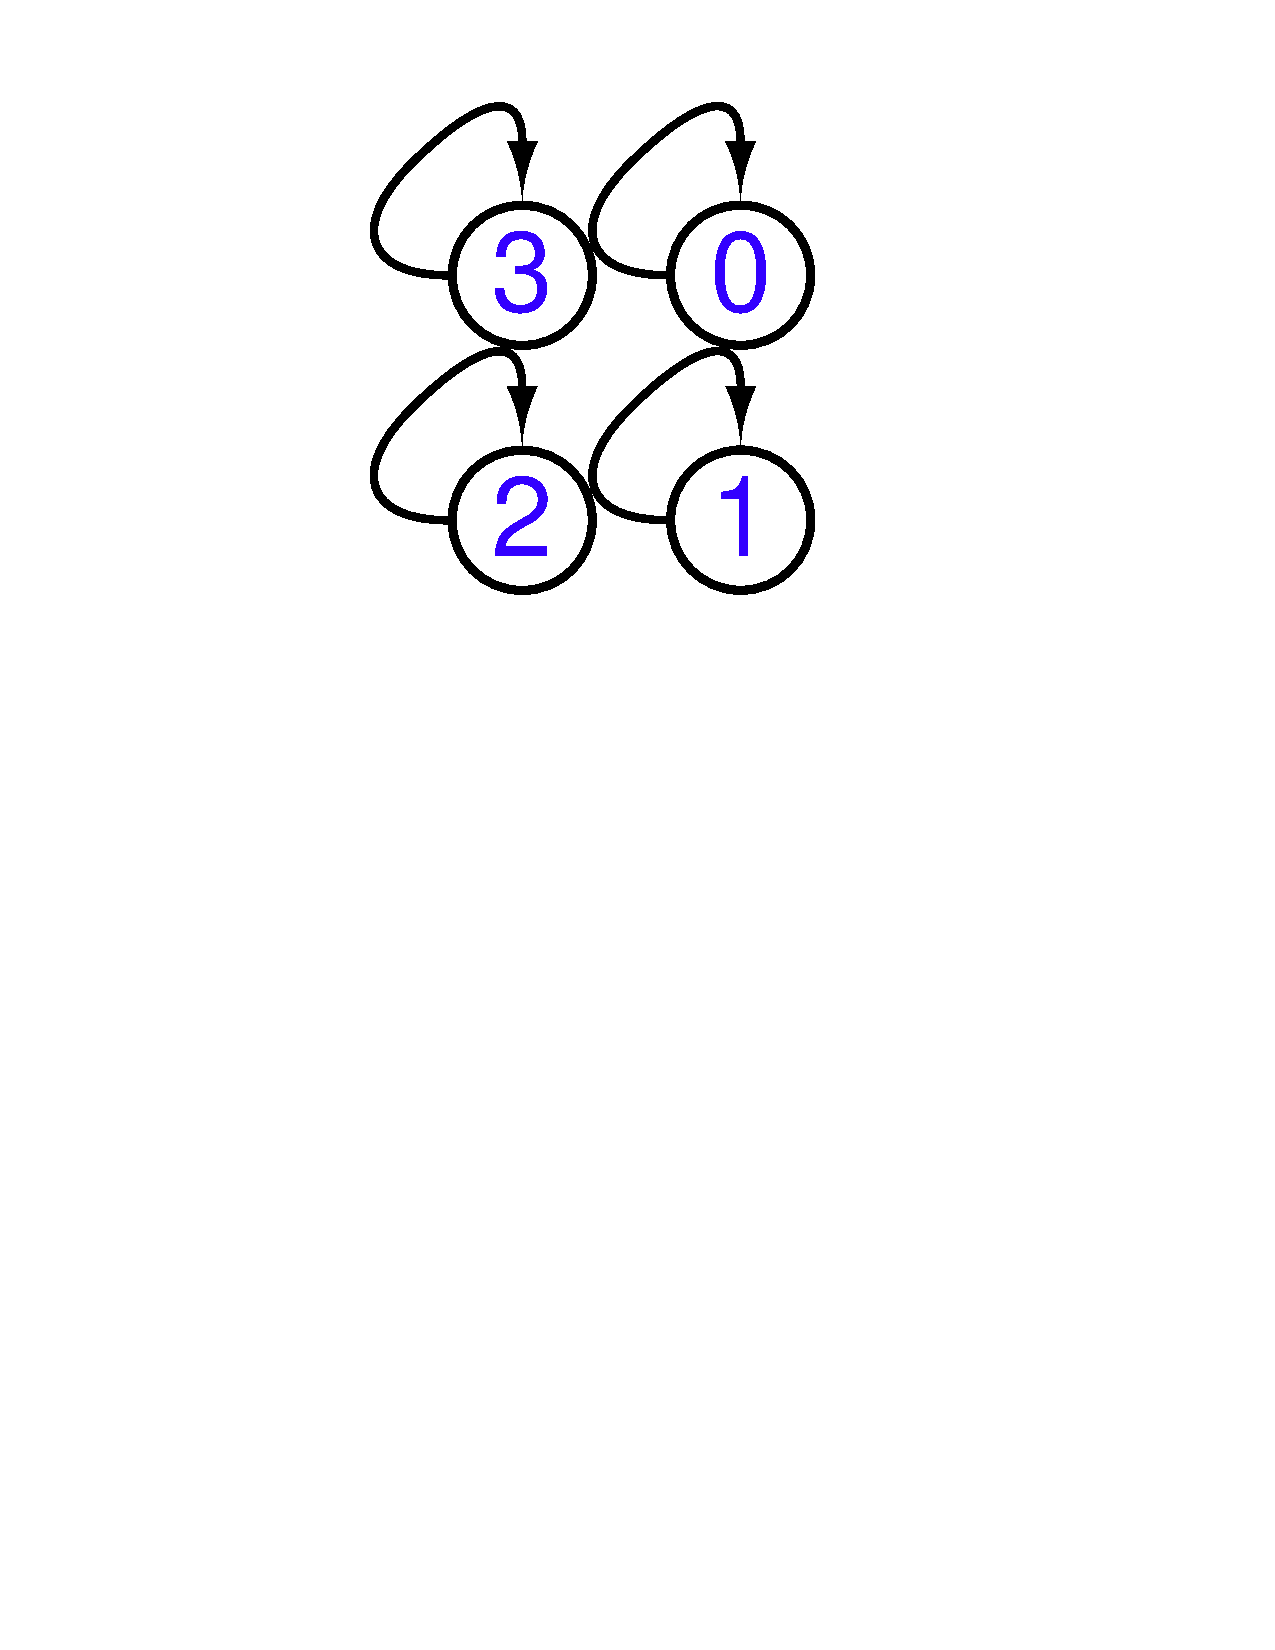
\includegraphics[width=0.77\FourImW]{a0_b0_e1}
		a)
	\end{minipage} \hspace*{\fill}
	\begin{minipage}{0.8\FourImW}
		\centering
		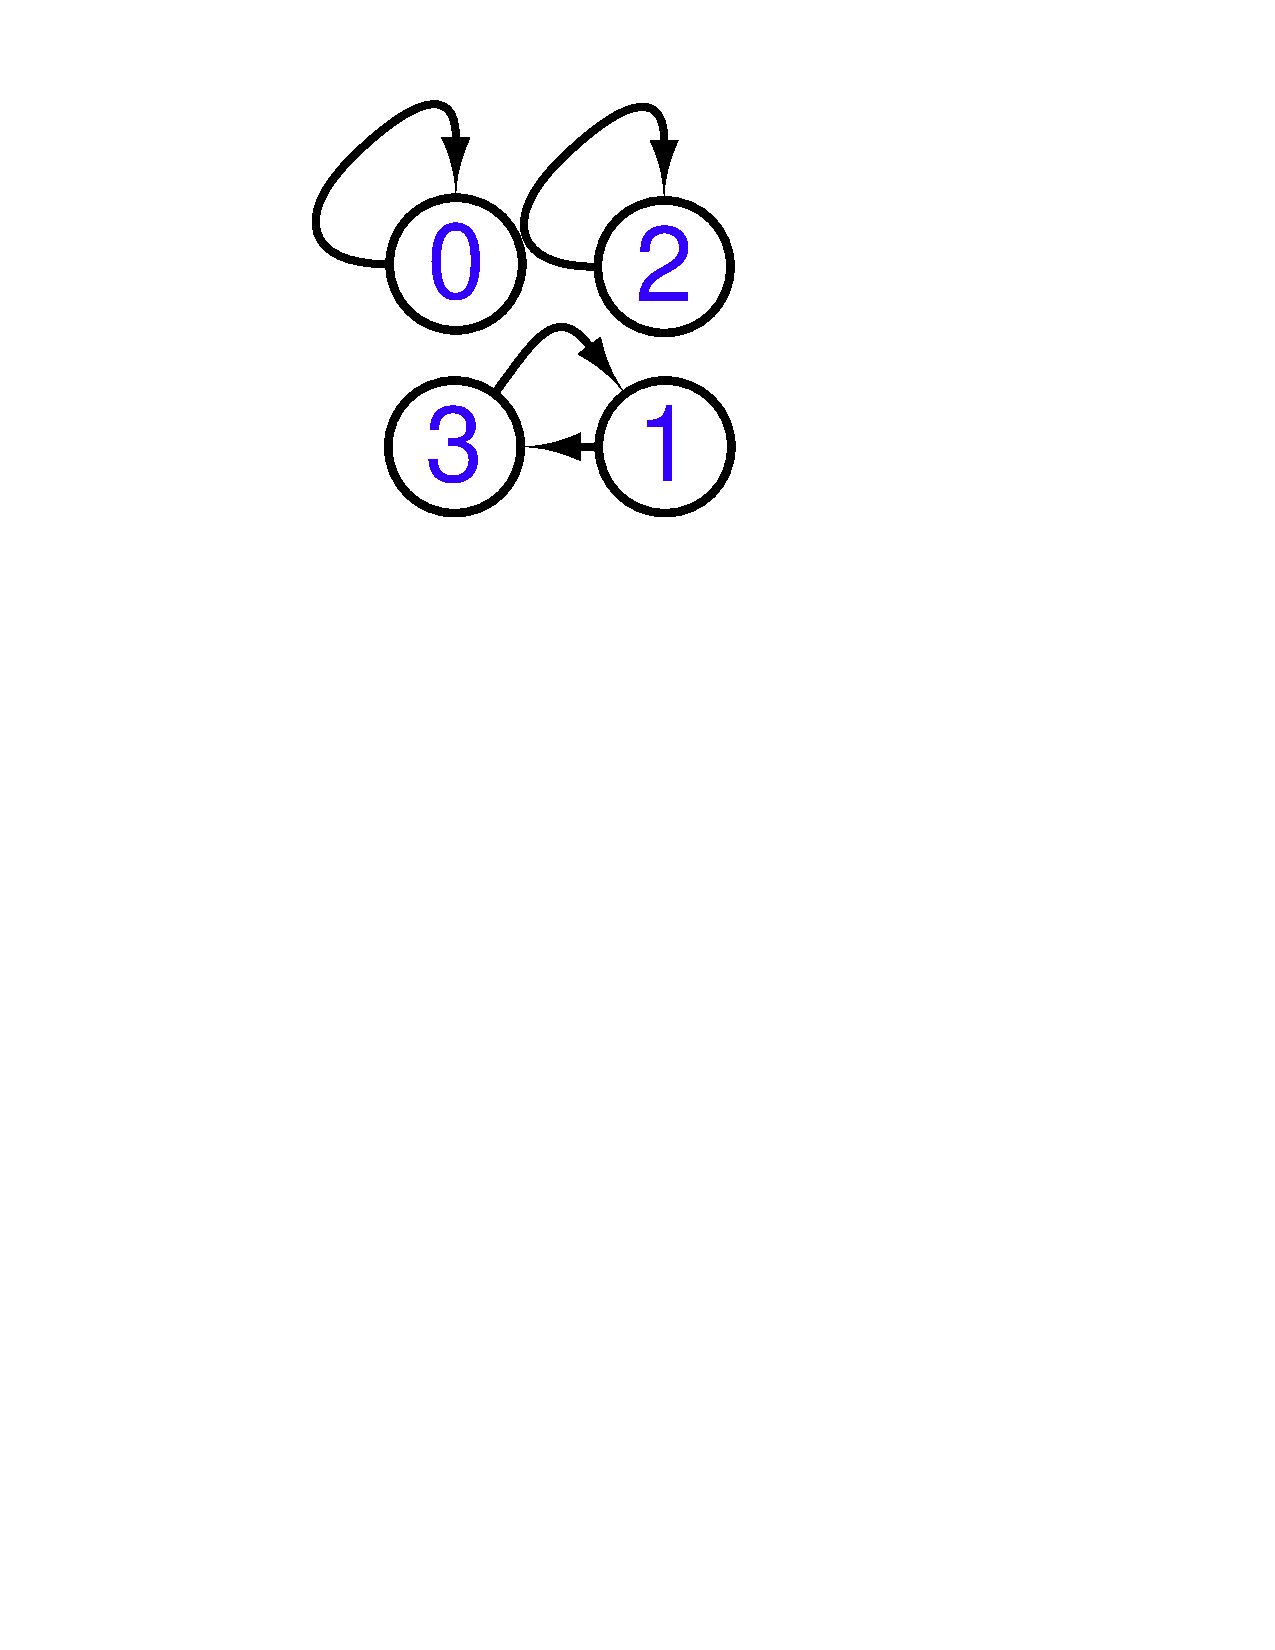
\includegraphics[width=0.8\FourImW]{a0_b1_e1}
		b)
	\end{minipage} \hspace*{\fill}
	\begin{minipage}{0.8\FourImW}
		\centering
		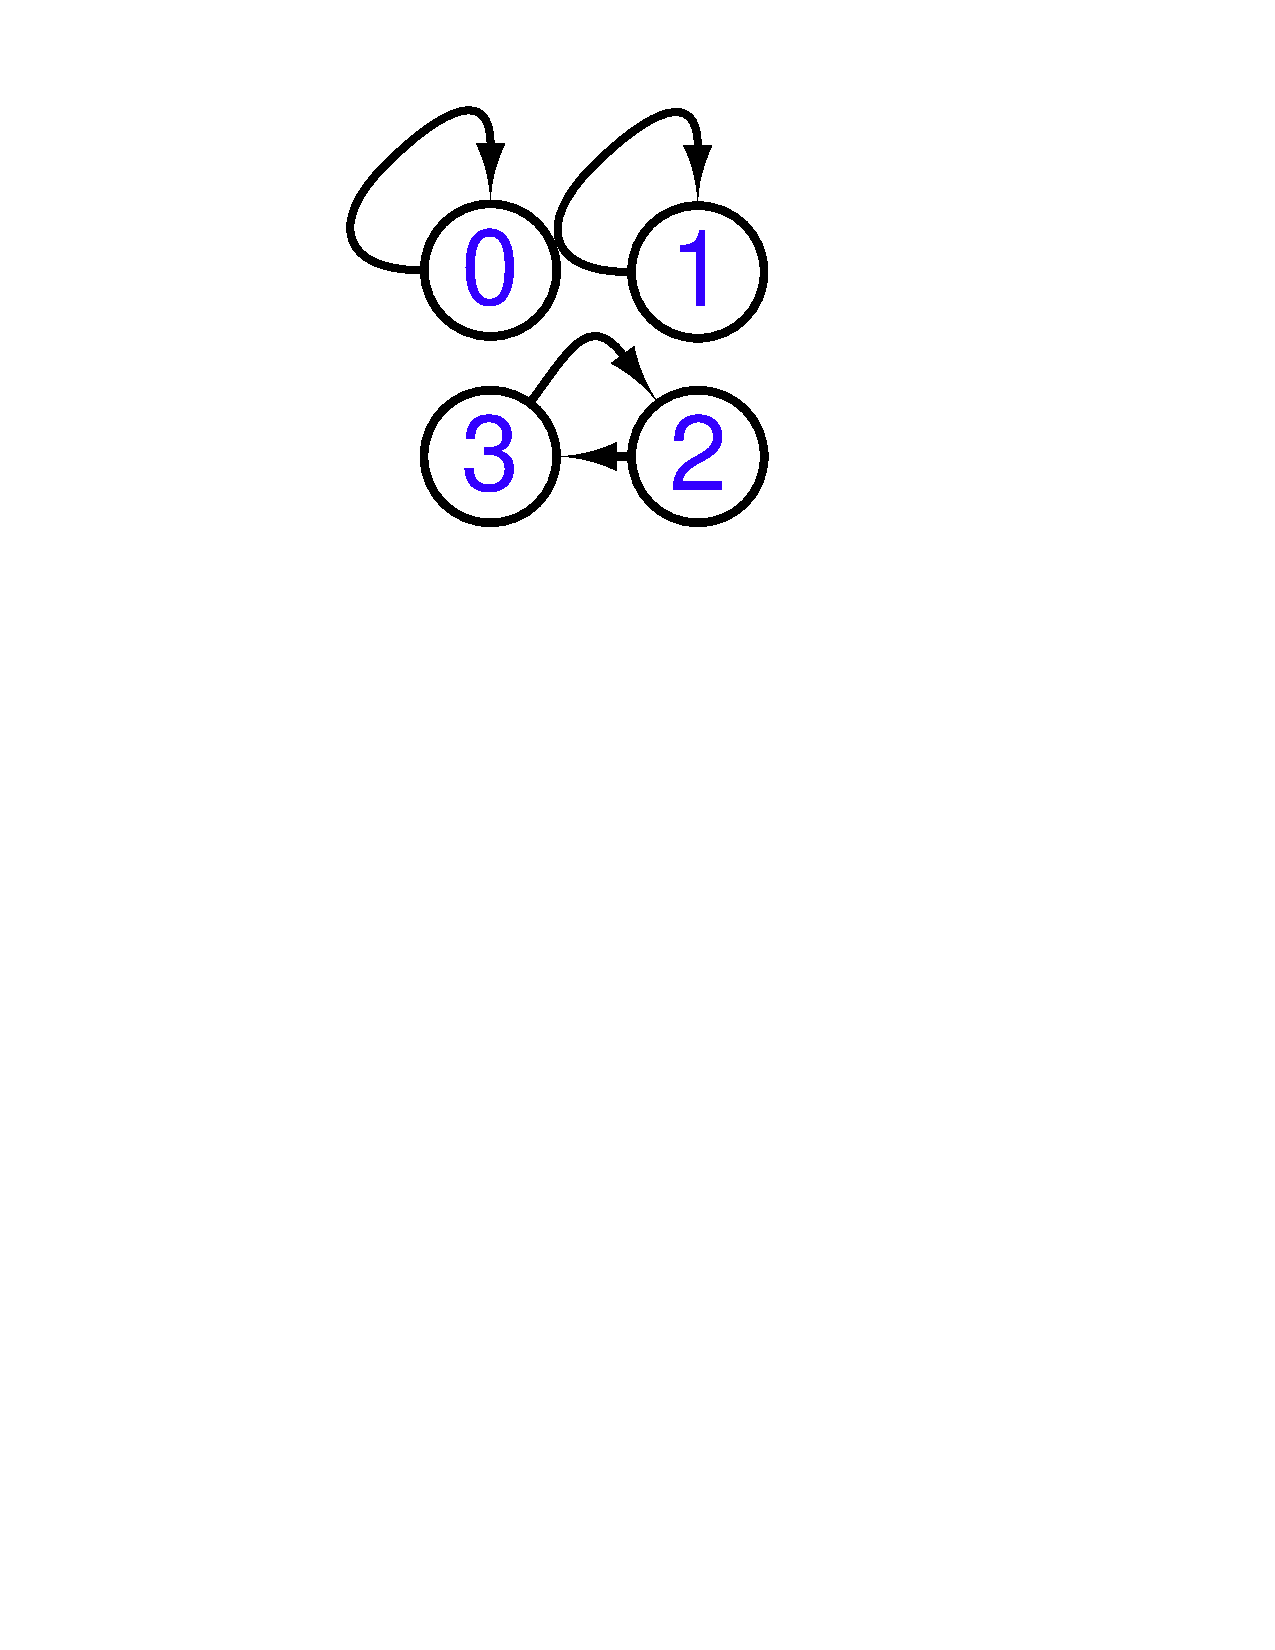
\includegraphics[width=0.8\FourImW]{a1_b0_e1}
		c)
	\end{minipage} \hspace*{\fill}
	\begin{minipage}{0.8\FourImW}
		\centering
		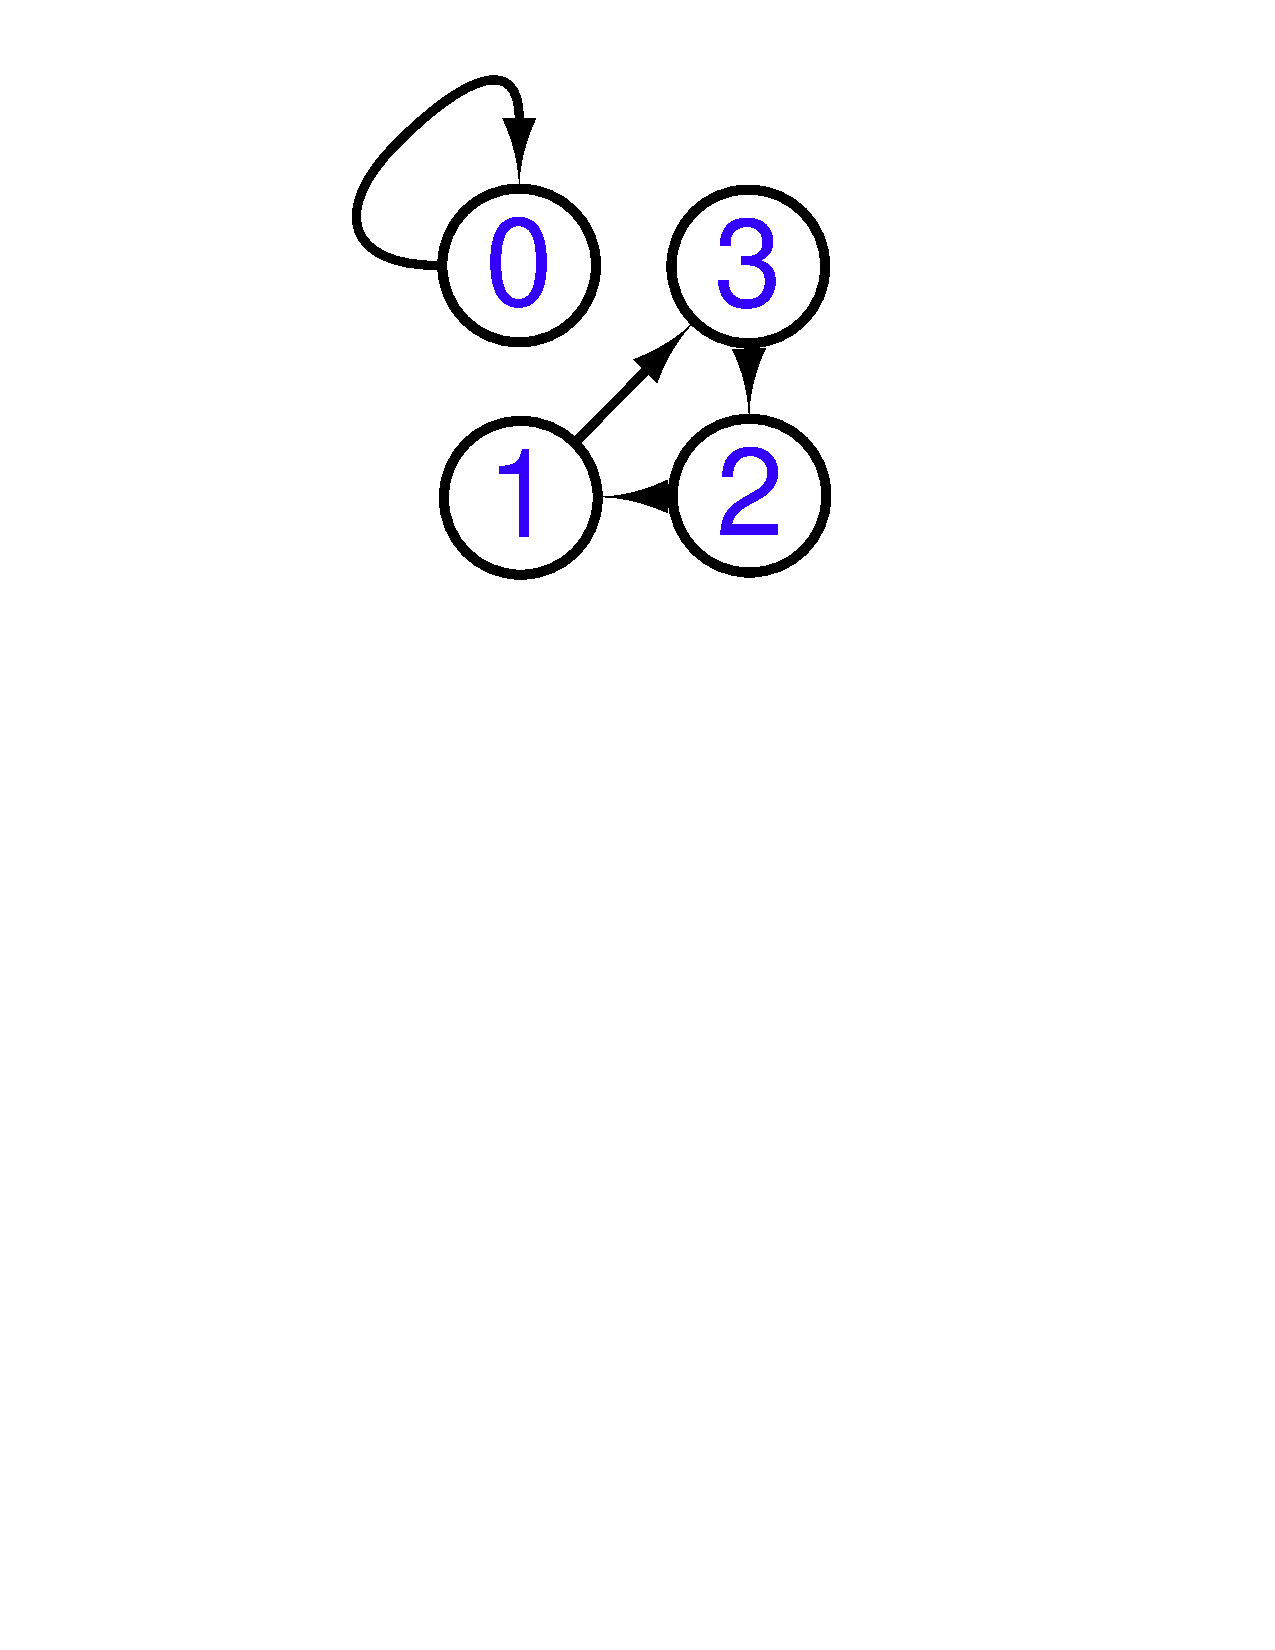
\includegraphics[width=0.8\FourImW]{a1_b1_e1}
		d)
	\end{minipage}
	\caption{$N=2$时,GDCM~(\ref{eq:ArnoldInteger})的4个可能状态映射网络:
		a) $p$ 和 $q$ 都为偶数; b) $p$ 为偶数,$q$ 为奇数;
		c) $p$ 为奇数,$q$ 为偶数; d) $p$ 和 $q$ 都为奇数}
	\label{fig:perioddistributione1}
\end{figure}

\begin{figure}[!htb]
\centering
\begin{minipage}{\FourImW}
\centering
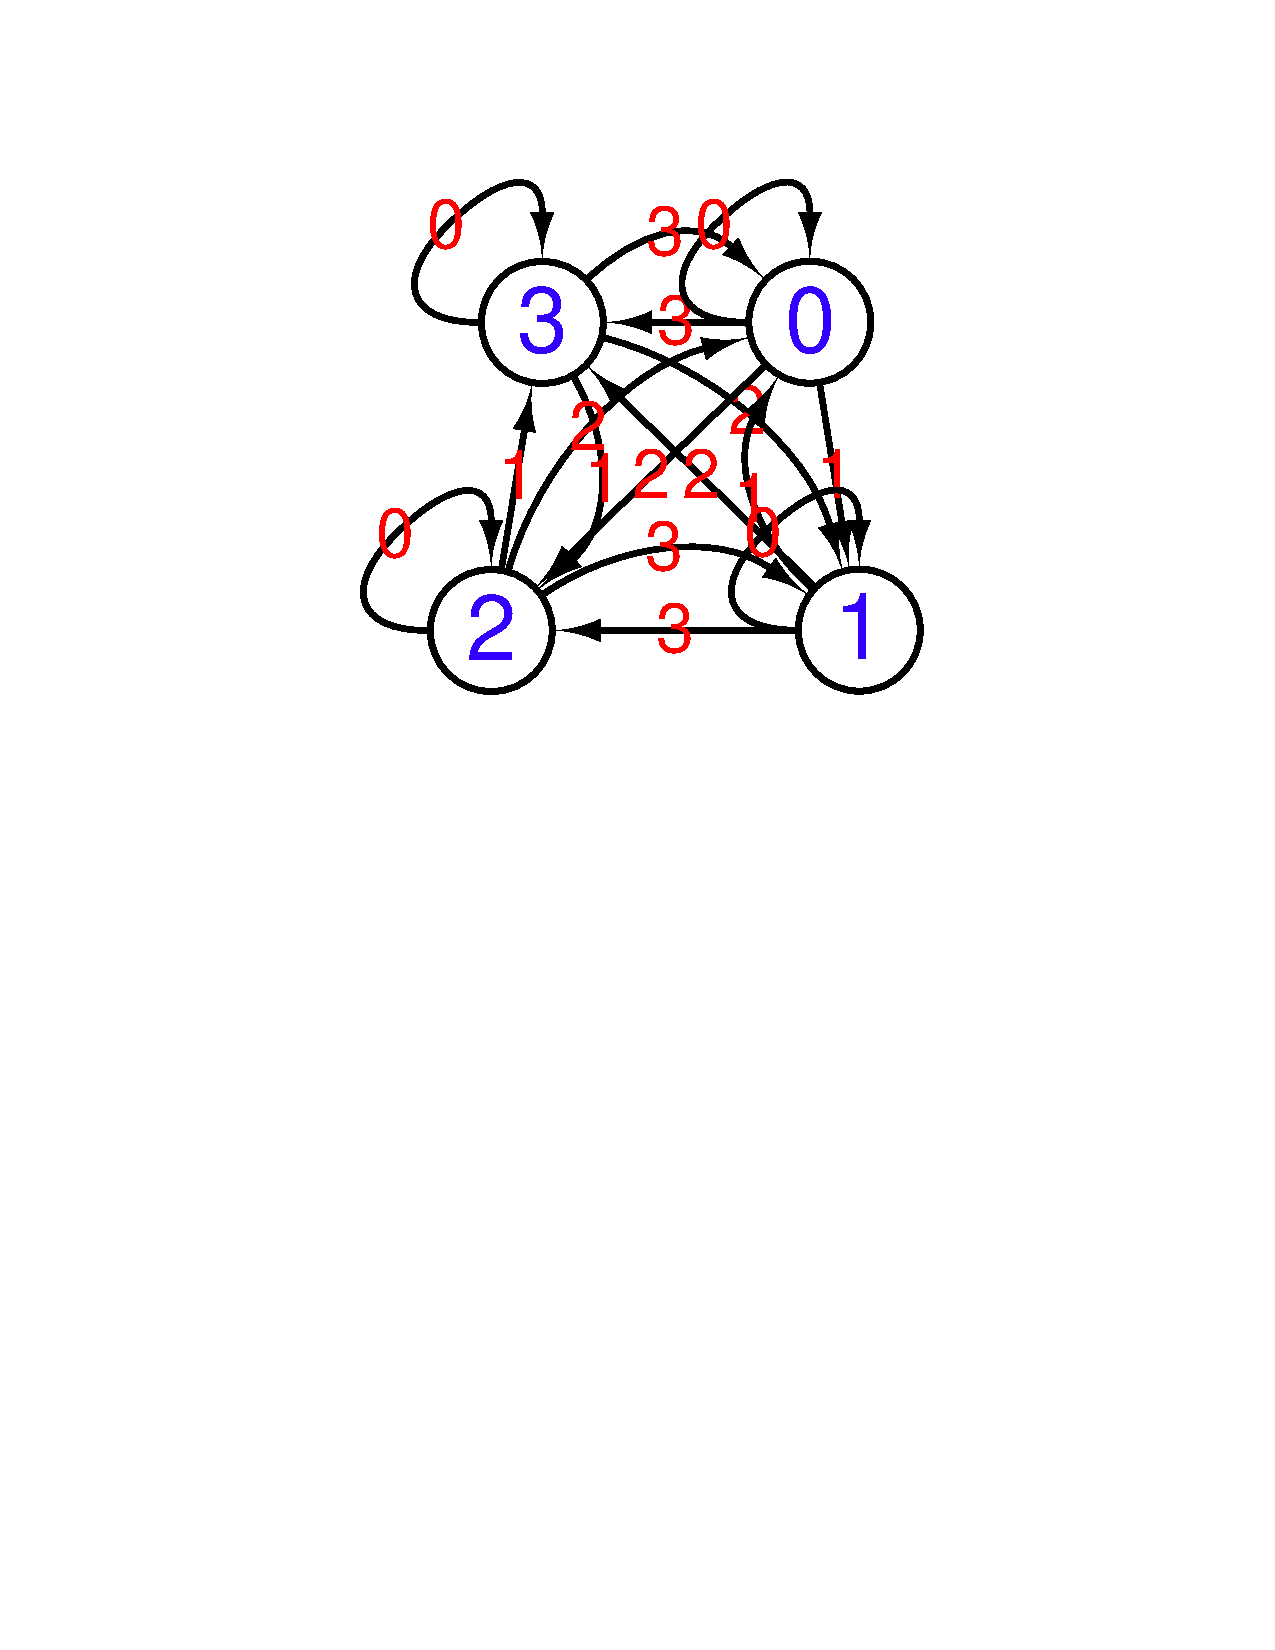
\includegraphics[width=\FourImW]{RootMap_00}
a)
\end{minipage}\hspace{0.9\figsep}
\begin{minipage}{\FourImW}
\centering
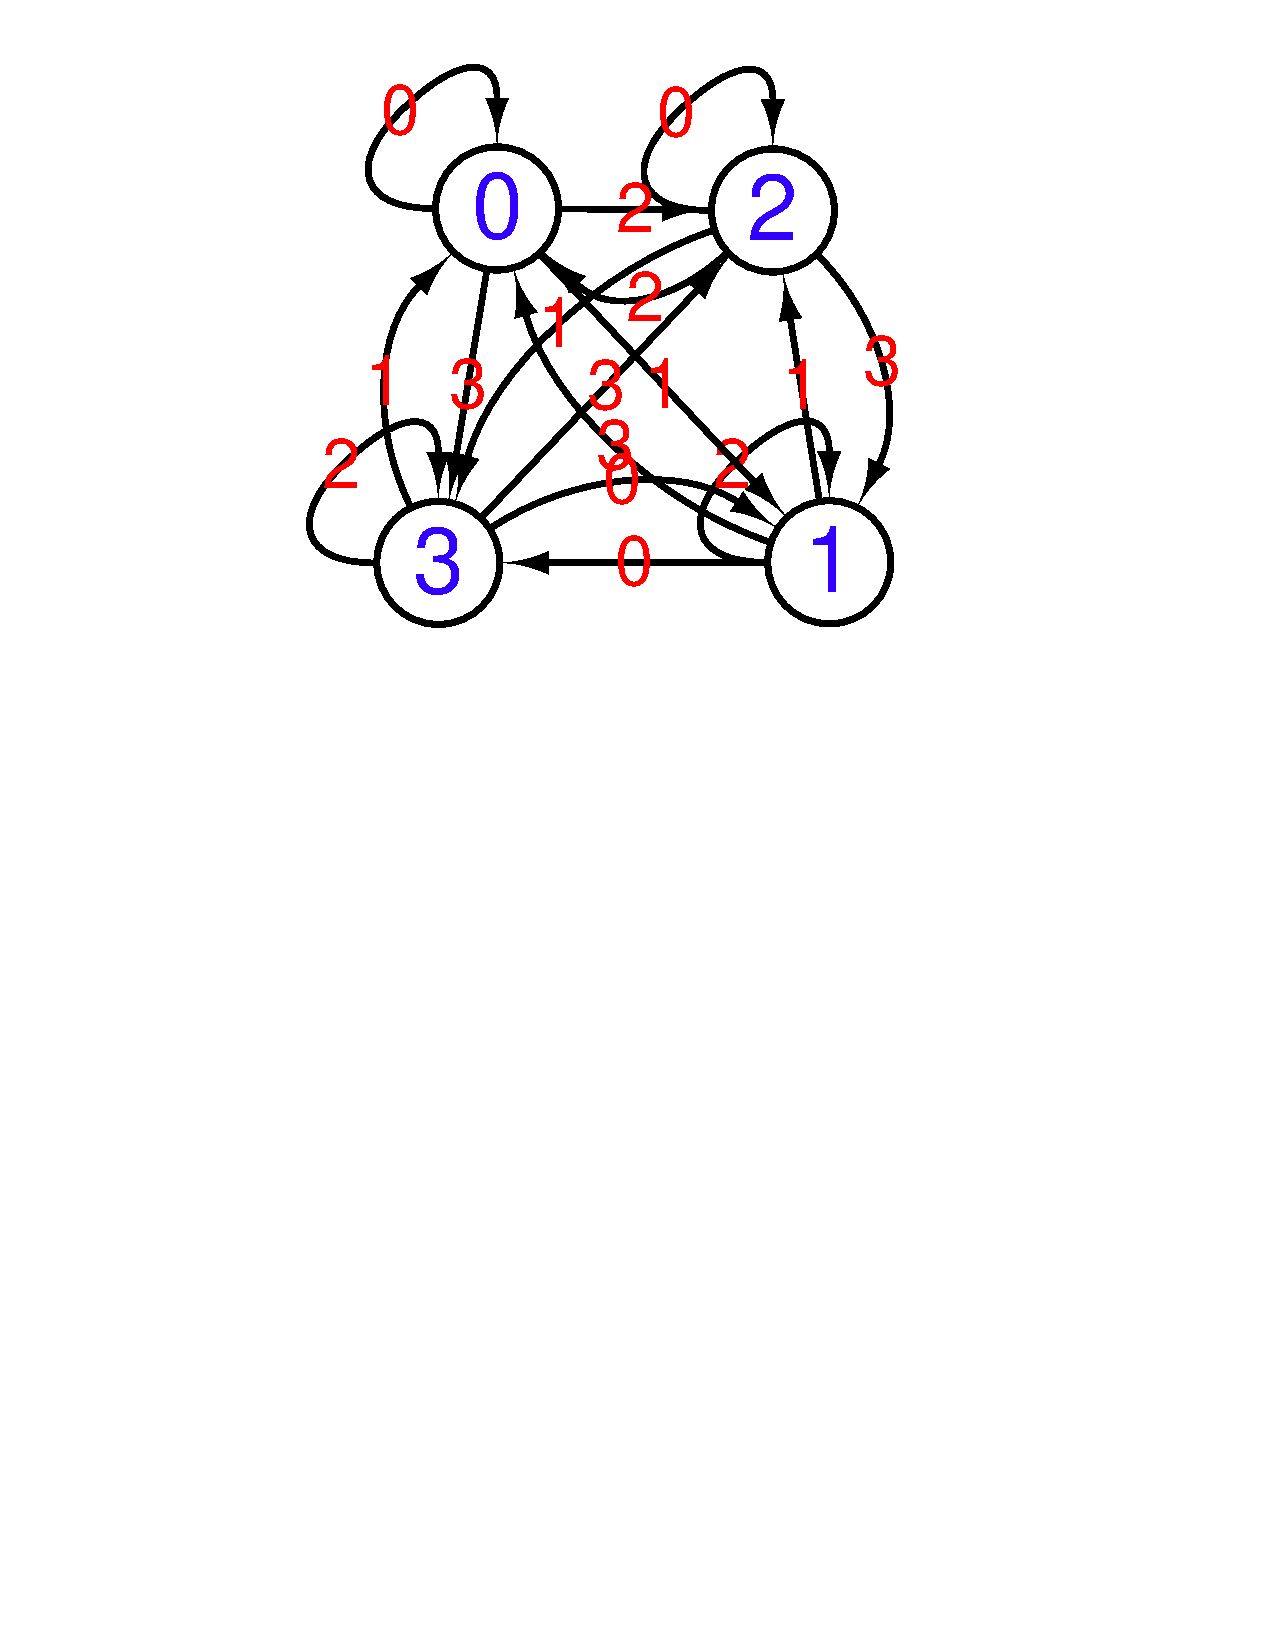
\includegraphics[width=\FourImW]{RootMap_01}
b)
\end{minipage}\hspace{0.9\figsep}
\begin{minipage}{\FourImW}
\centering
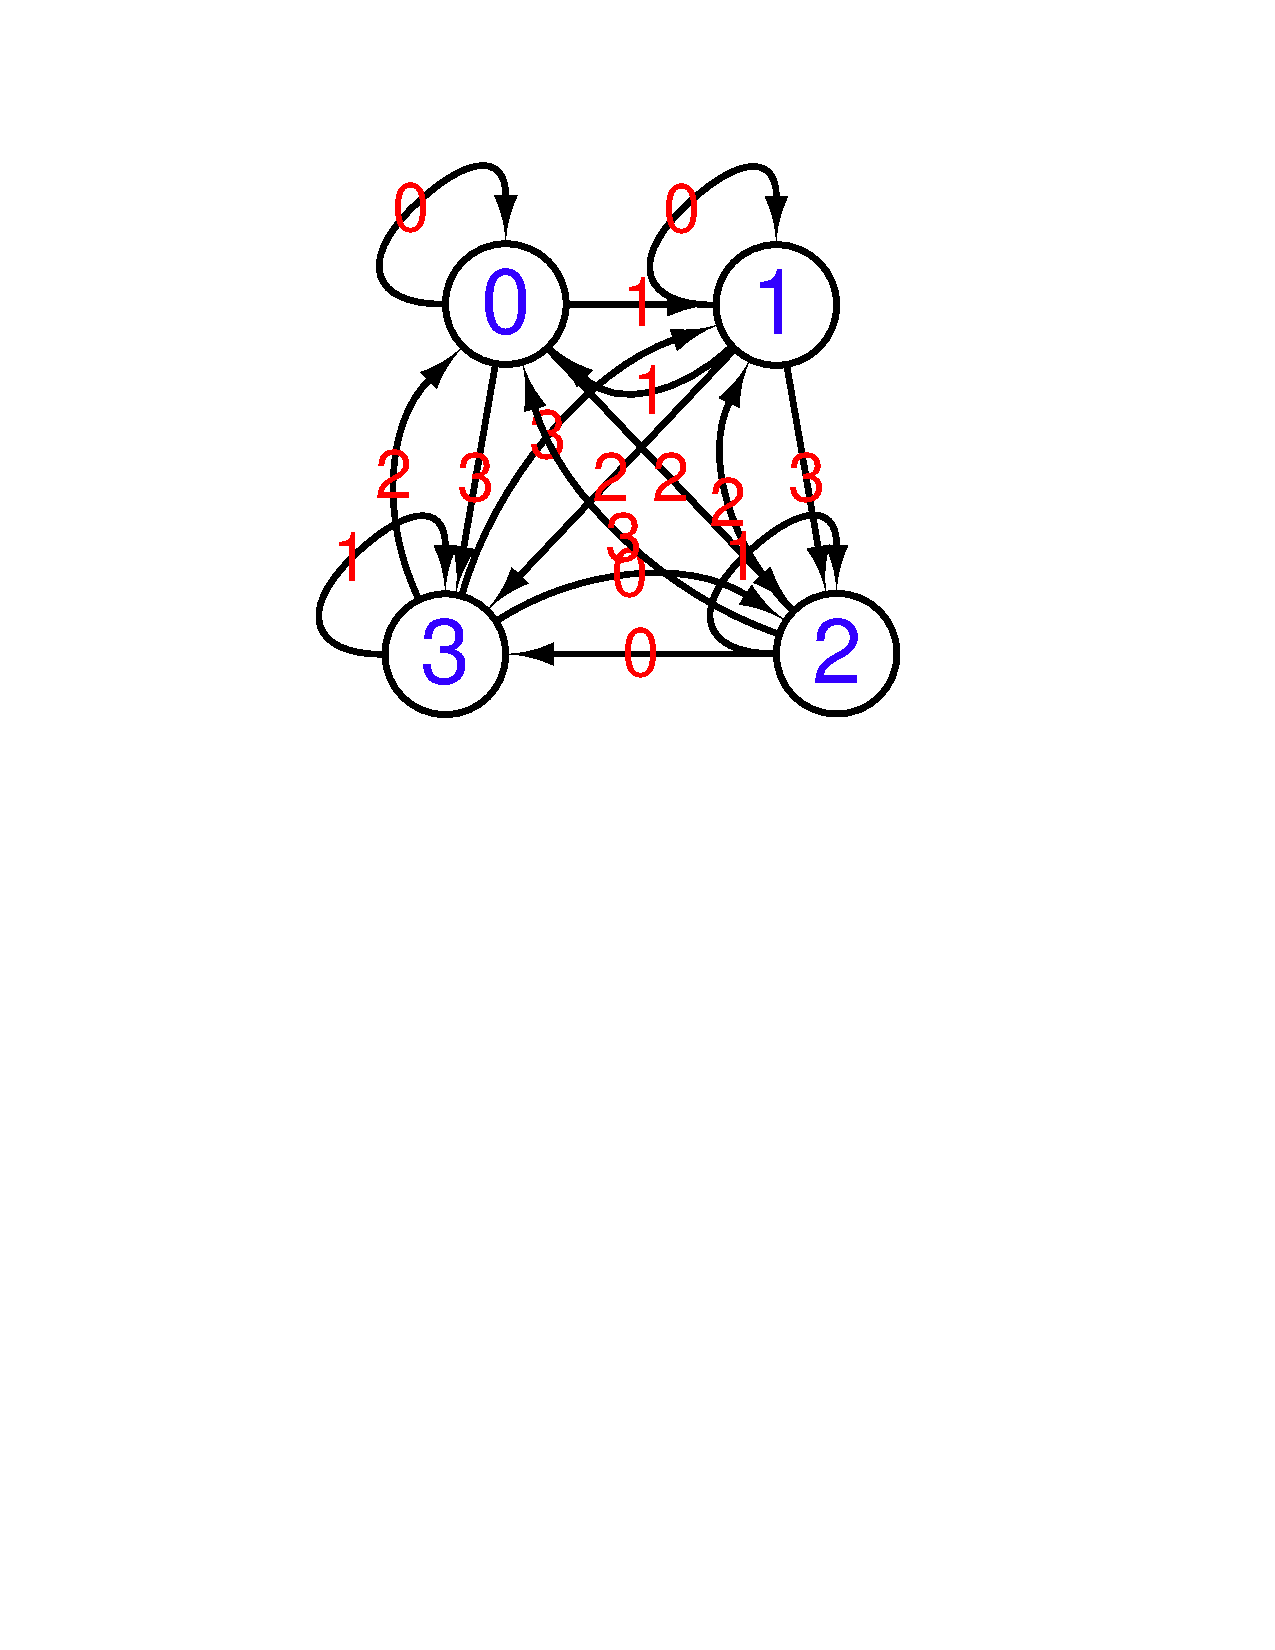
\includegraphics[width=\FourImW]{RootMap_10}
c)
\end{minipage}\hspace{0.9\figsep}
\begin{minipage}{1.1\FourImW}
\centering
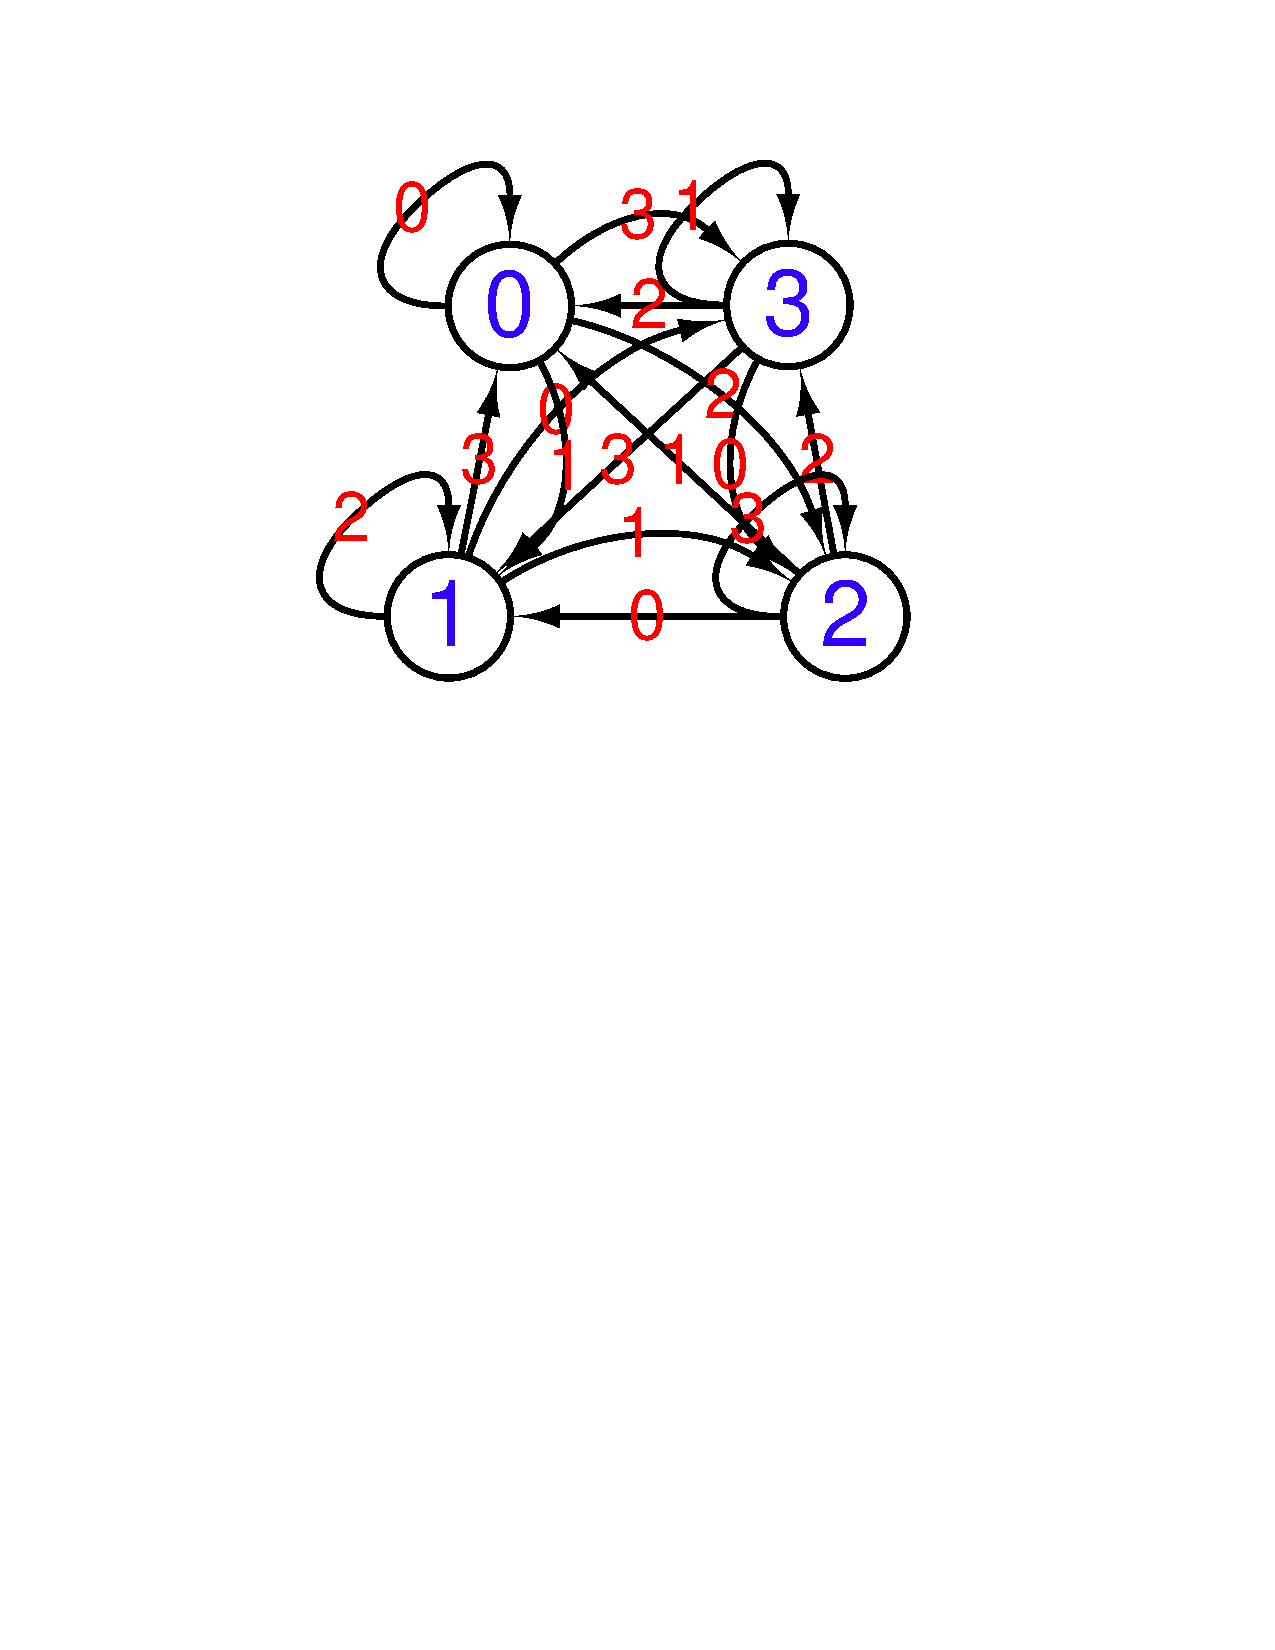
\includegraphics[width=1.1\FourImW]{RootMap_11}
d)
\end{minipage}
\caption{(\ref{eq:kxky})式中$(a_n+2b_n)$与$(a_{n+1}+2b_{n+1})$之间的映射,箭头旁边所示为$(k_x+2k_y)$的值:
a) $p$ 和 $q$ 都为偶数; b) $p$ 为偶数,$q$ 为奇数;
c) $p$ 为奇数,$q$ 为偶数; d) $p$ 和 $q$ 都为奇数}
\label{fig:rootmap}
\end{figure}

\begin{Property}
GDCM~(\ref{eq:ArnoldInteger})定义集合$(0, 1, 2, \cdots, N^{2}-1)$上的双射。
\label{prop:bijective}
\end{Property}
\begin{proof}
因为Cat映射~\eqref{eq:ArnoldInteger}为保面积映射,所以其为有限域$\mathbb{Z}^2_{N}$上的双射,
根据~(\ref{eq:quantization})式,Cat映射可进一步转换为有限域$\mathbb{Z}_{N^2}$上的双射。\qedsymbol
\end{proof}

\begin{figure}[!htb]
\centering
\begin{minipage}[b]{\FourImW}
\centering
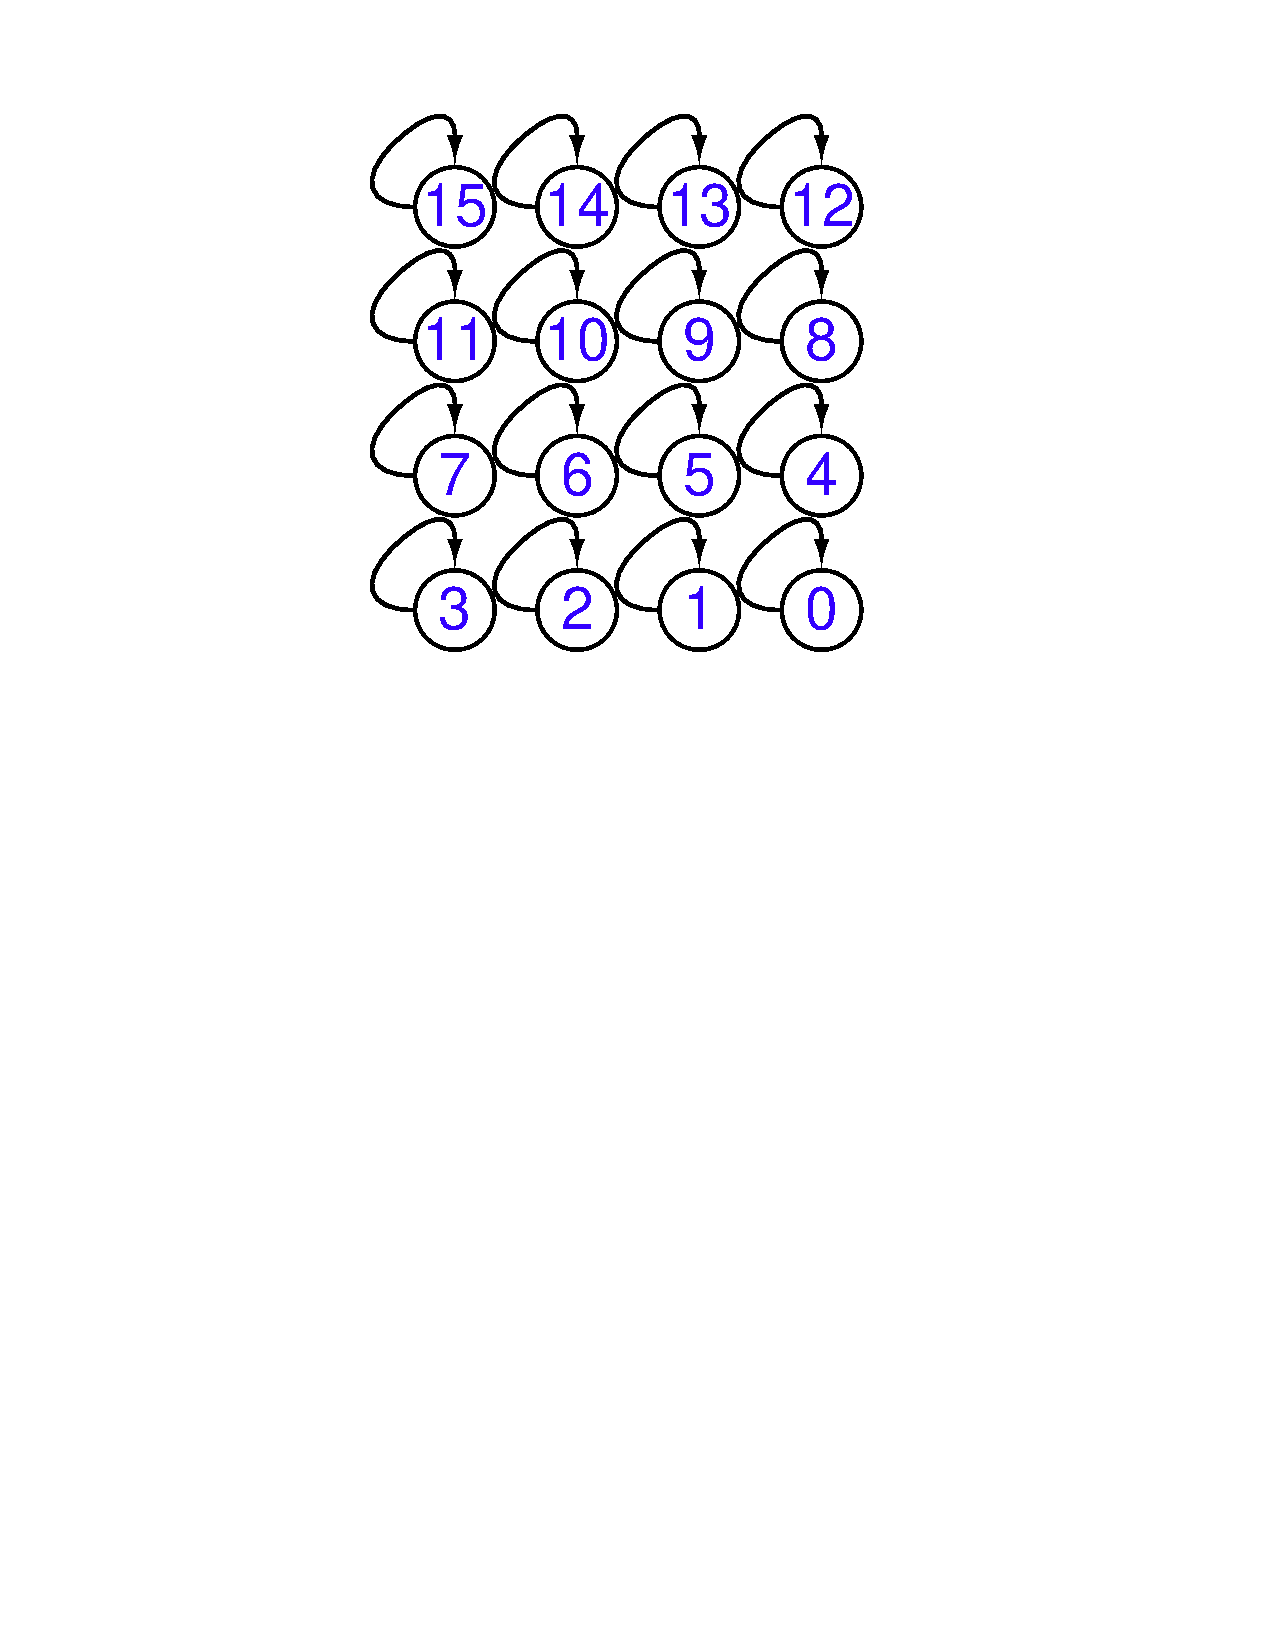
\includegraphics[keepaspectratio,width=\FourImW,height=\FourImW]{a0_b0_e2}
0)
\end{minipage}
\begin{minipage}[b]{\FourImW}
\centering
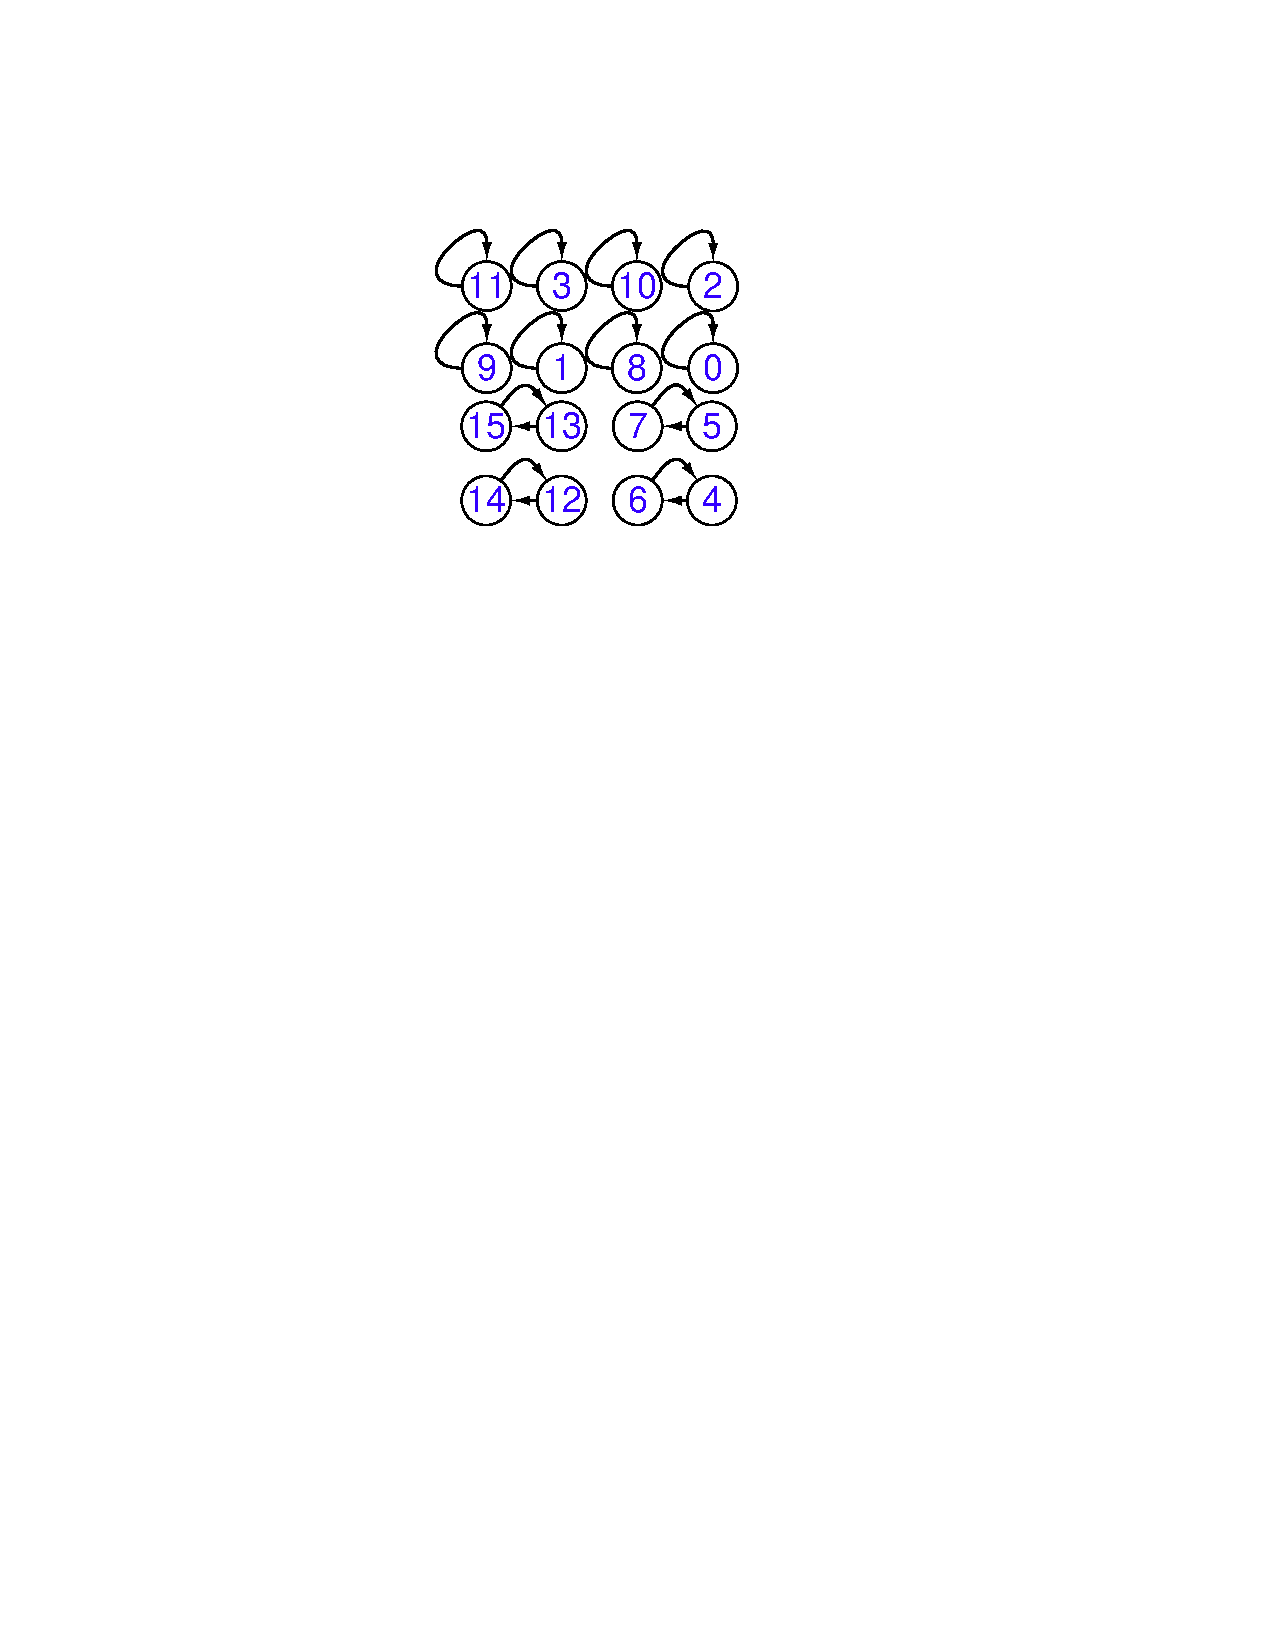
\includegraphics[width=\FourImW]{a2_b0_e2}
2)
\end{minipage}
\begin{minipage}[b]{\FourImW}
\centering
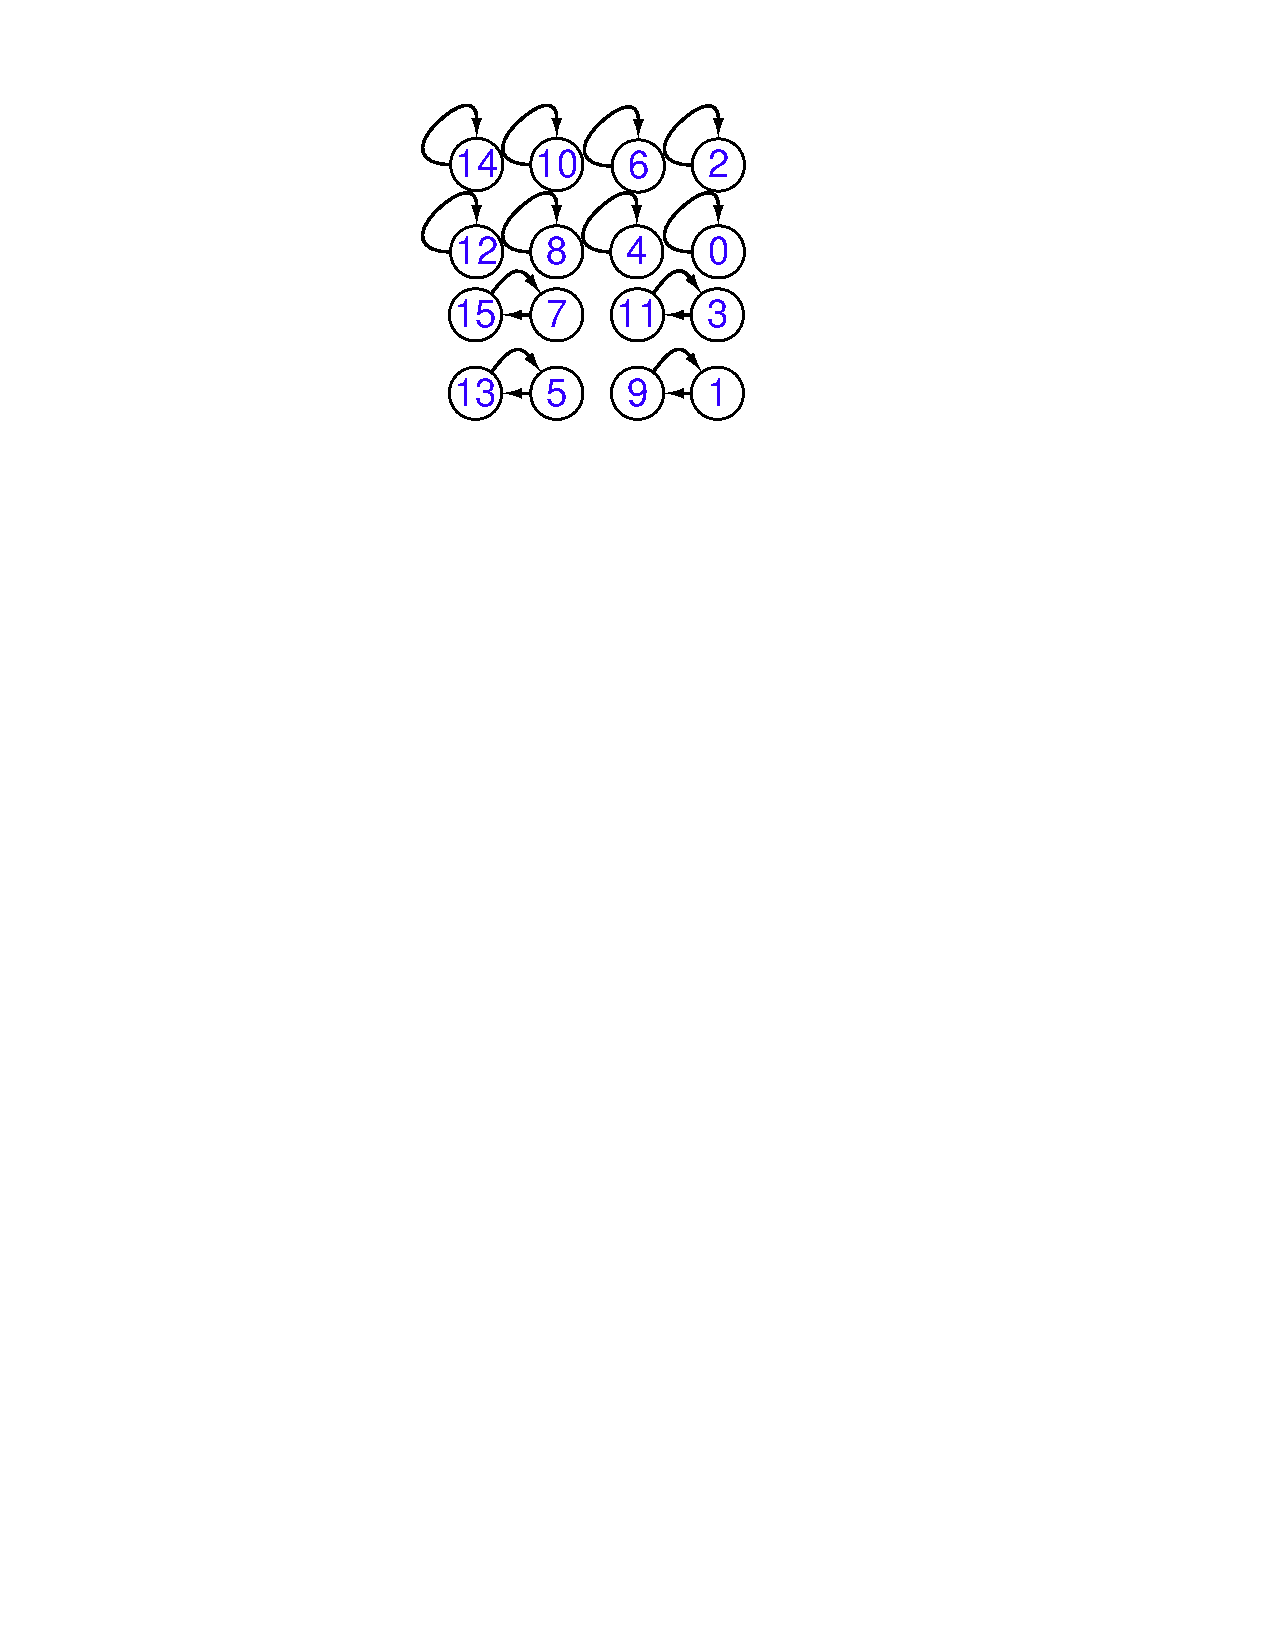
\includegraphics[width=\FourImW]{a0_b2_e2}
8)
\end{minipage}
\begin{minipage}[b]{\FourImW}
\centering
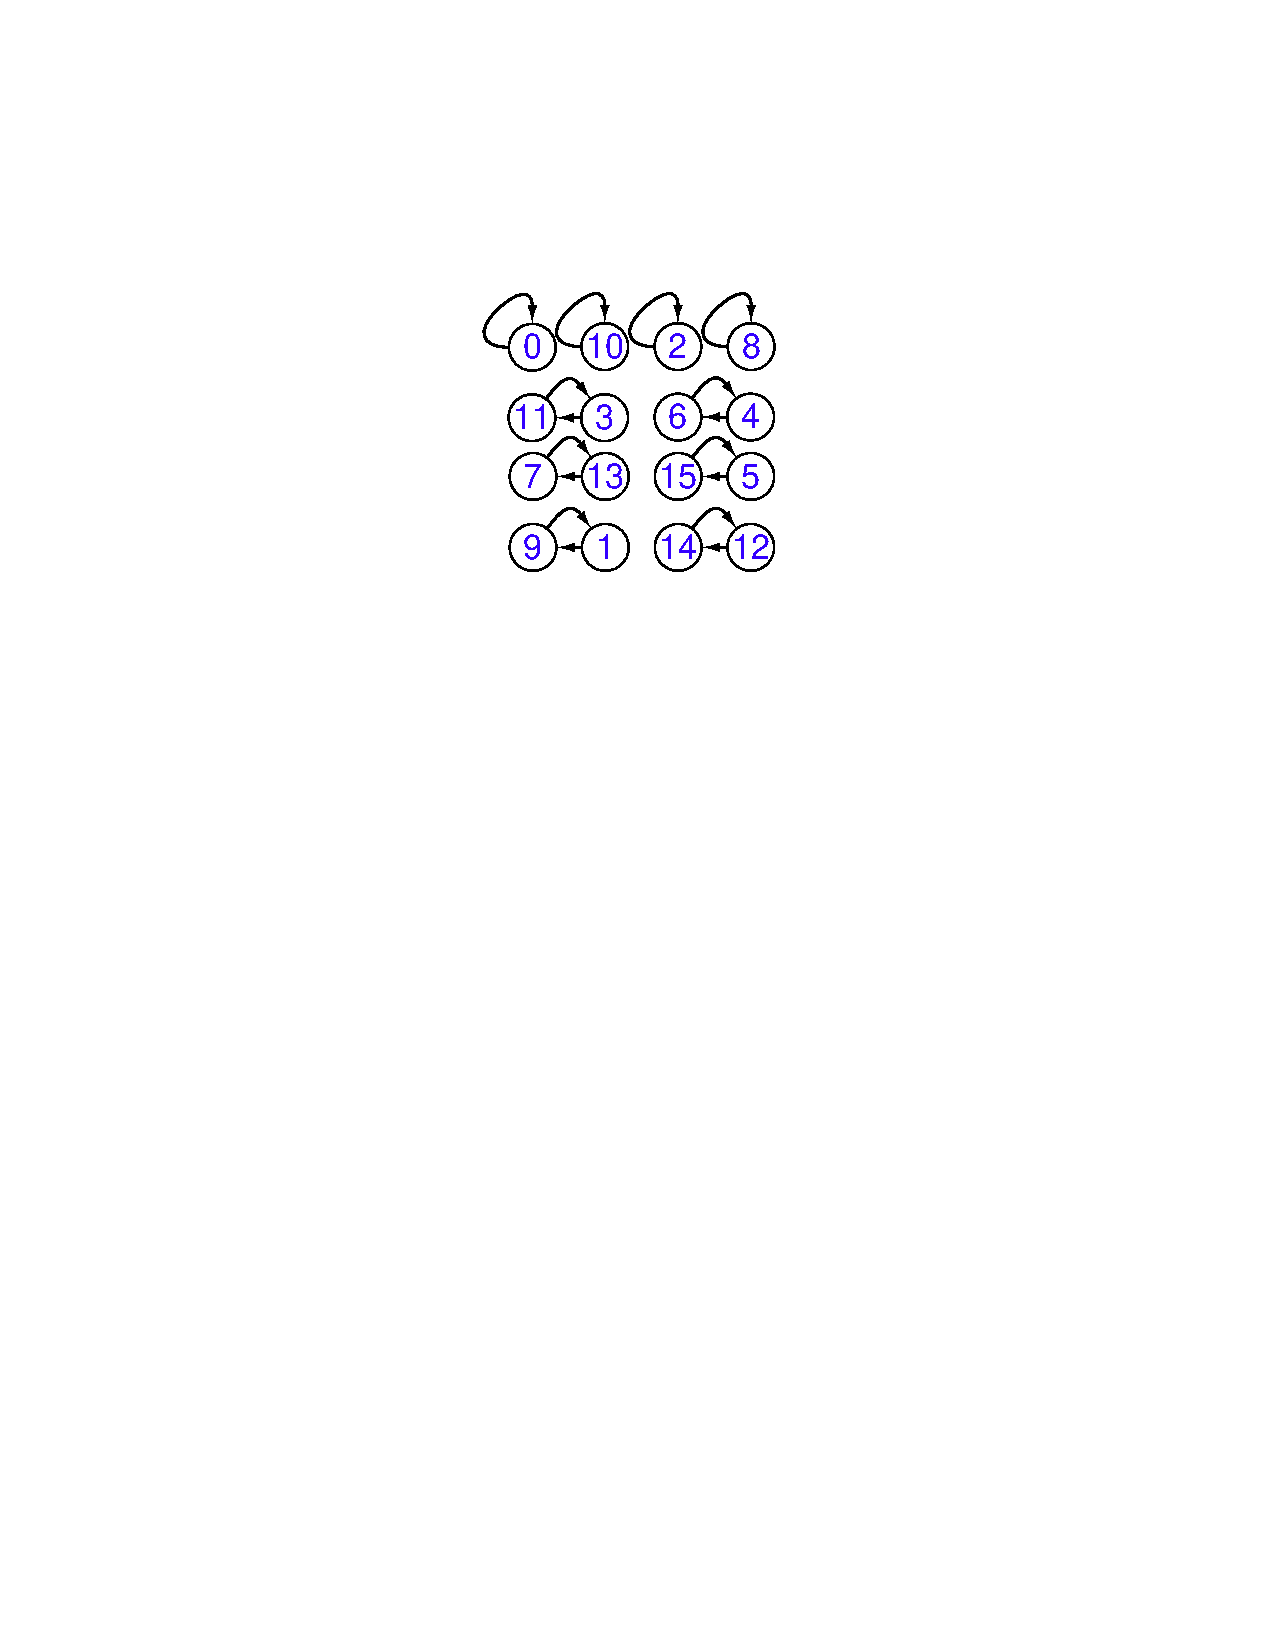
\includegraphics[width=\FourImW]{a2_b2_e2}
10)
\end{minipage}\\
\begin{minipage}[b]{\FourImW}
\centering
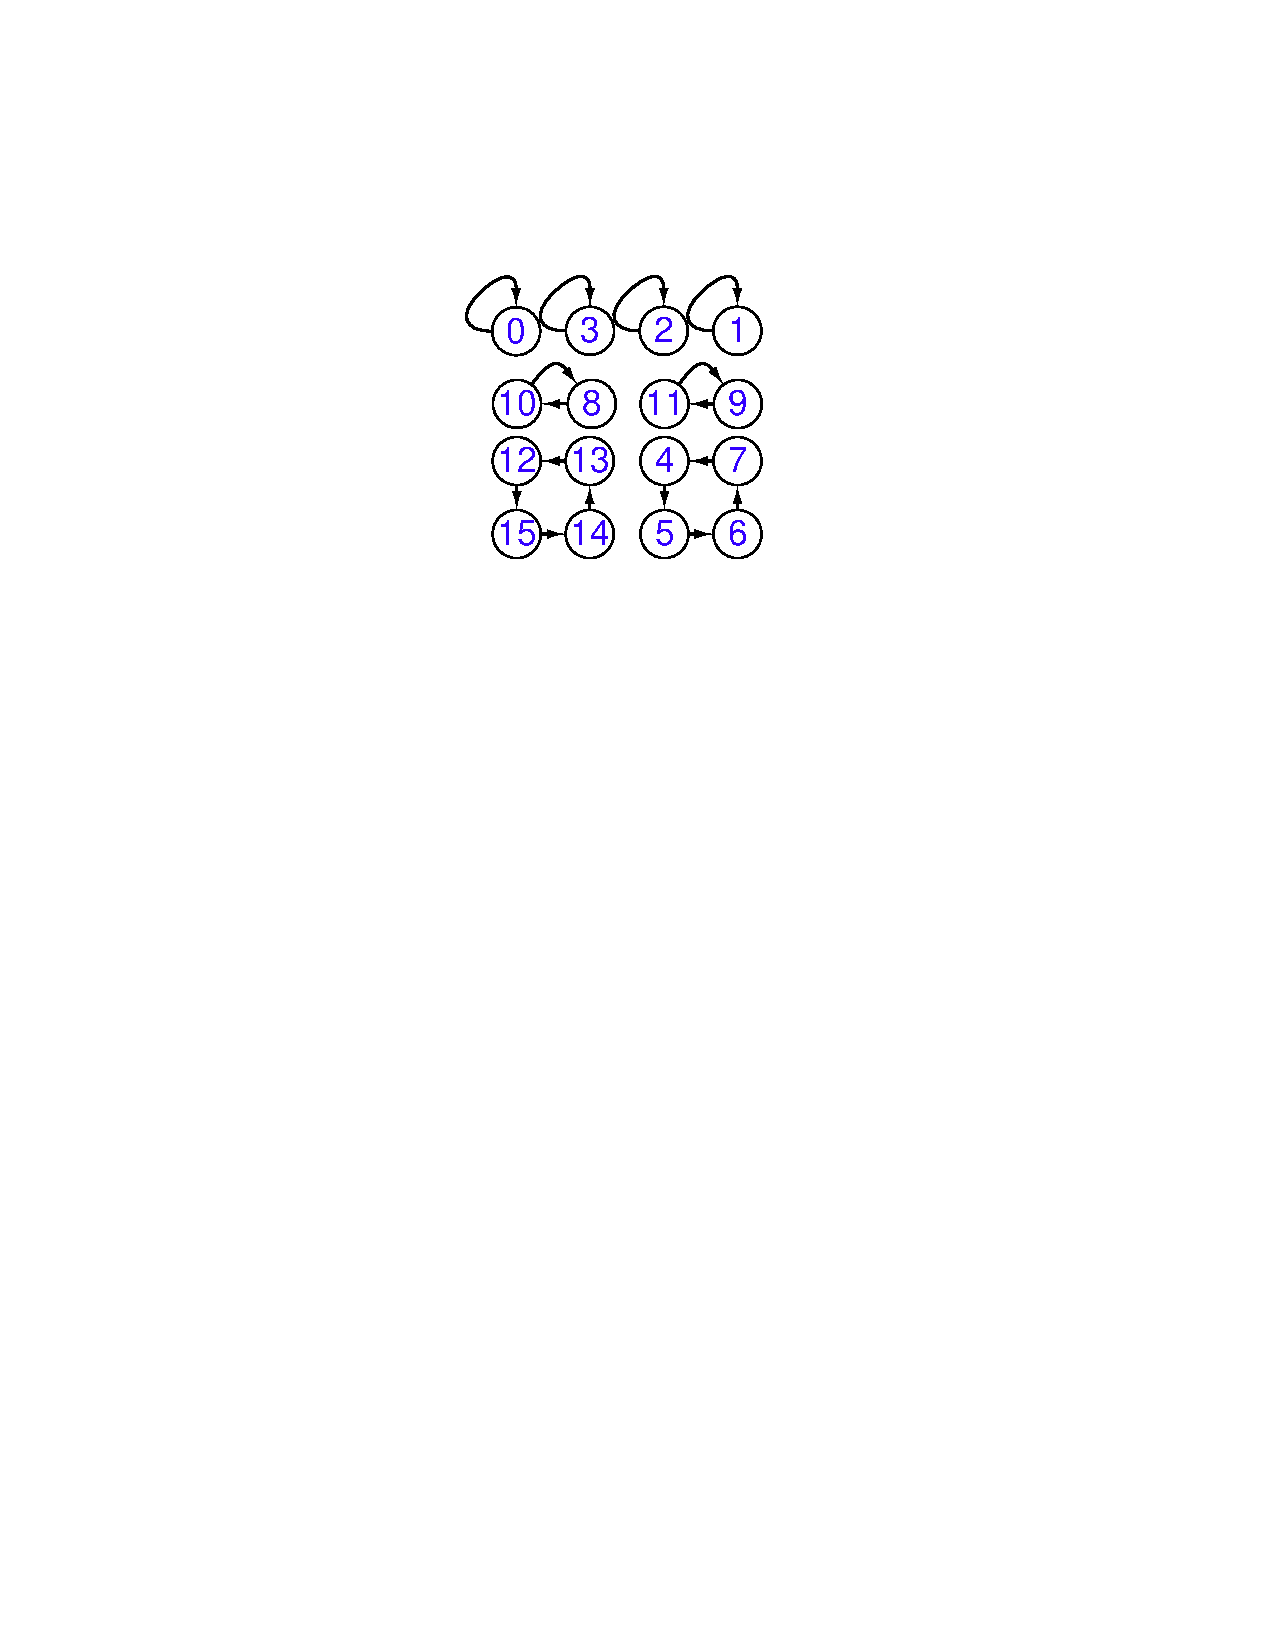
\includegraphics[width=\FourImW]{a1_b0_e2}
1)
\end{minipage}
\begin{minipage}[b]{\FourImW}
\centering
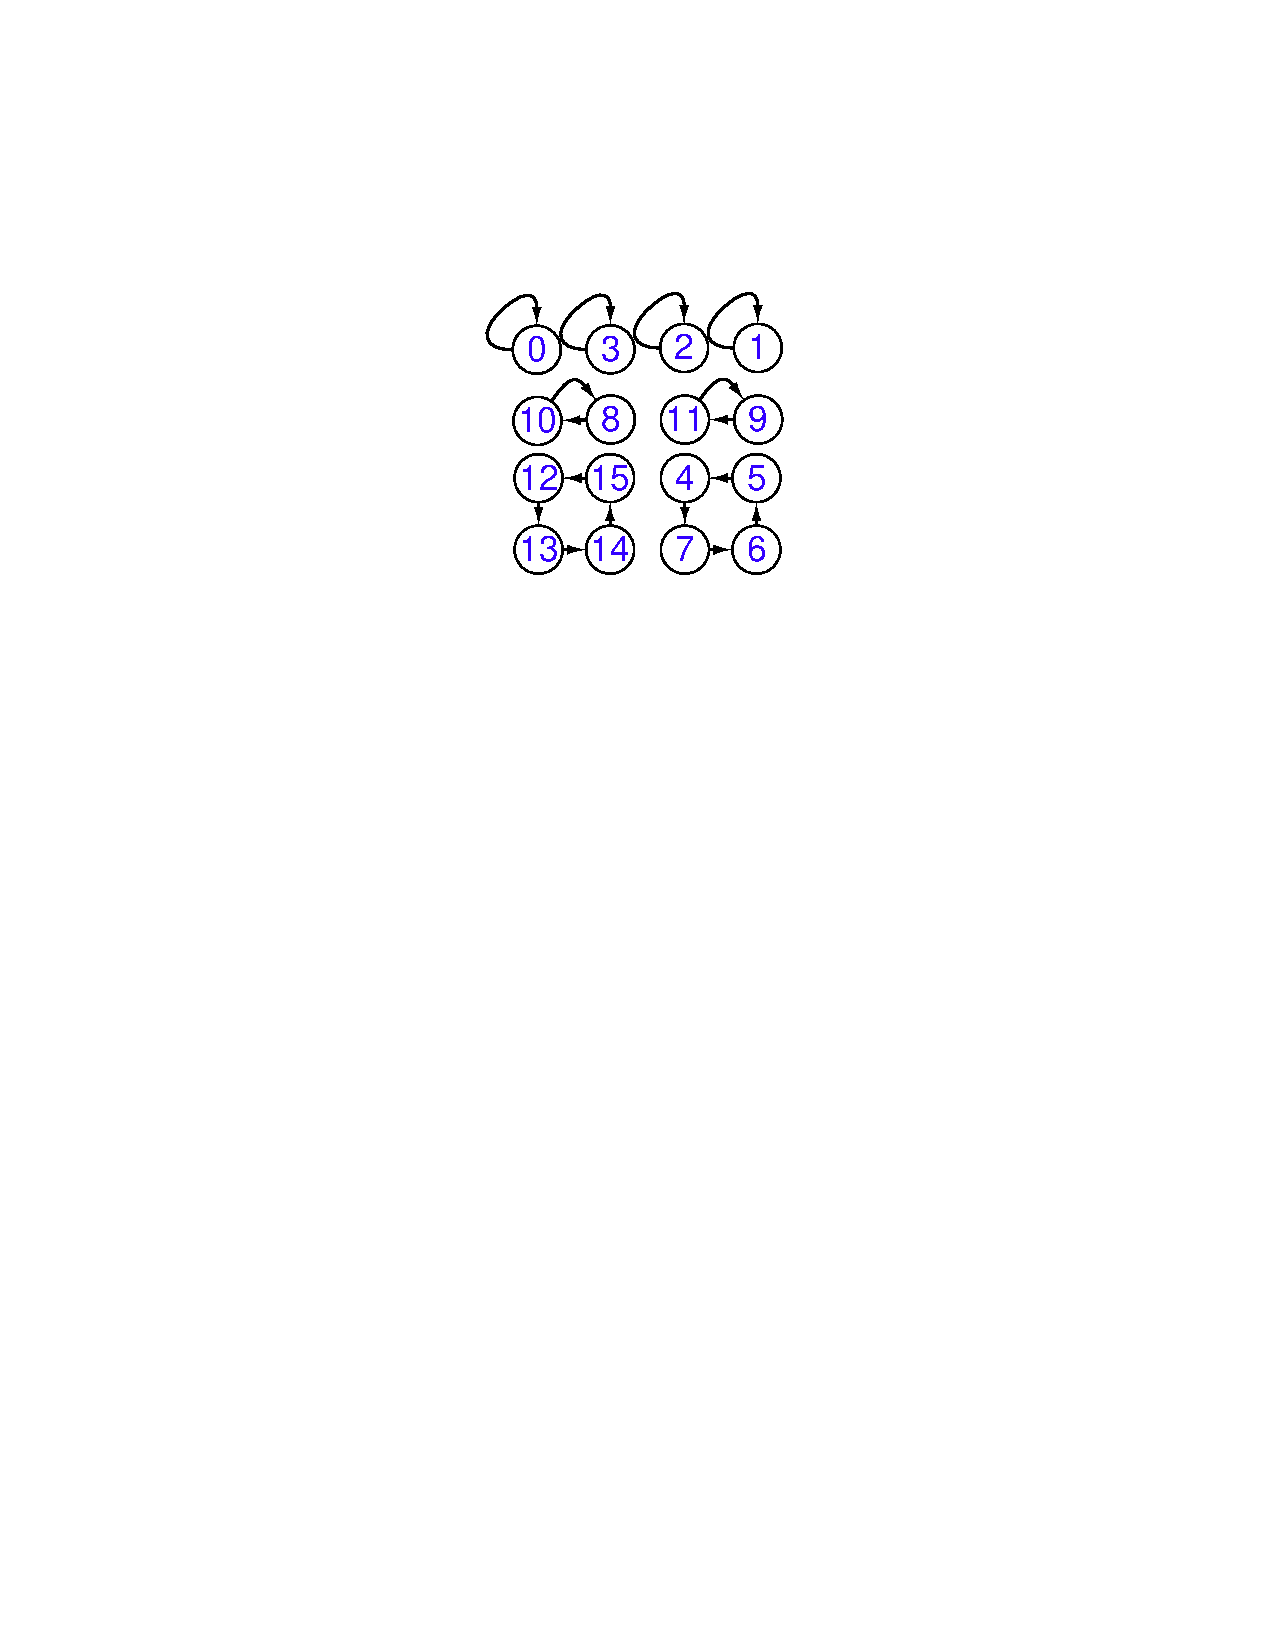
\includegraphics[width=\FourImW]{a3_b0_e2}
3)
\end{minipage}
\begin{minipage}[b]{\FourImW}
\centering
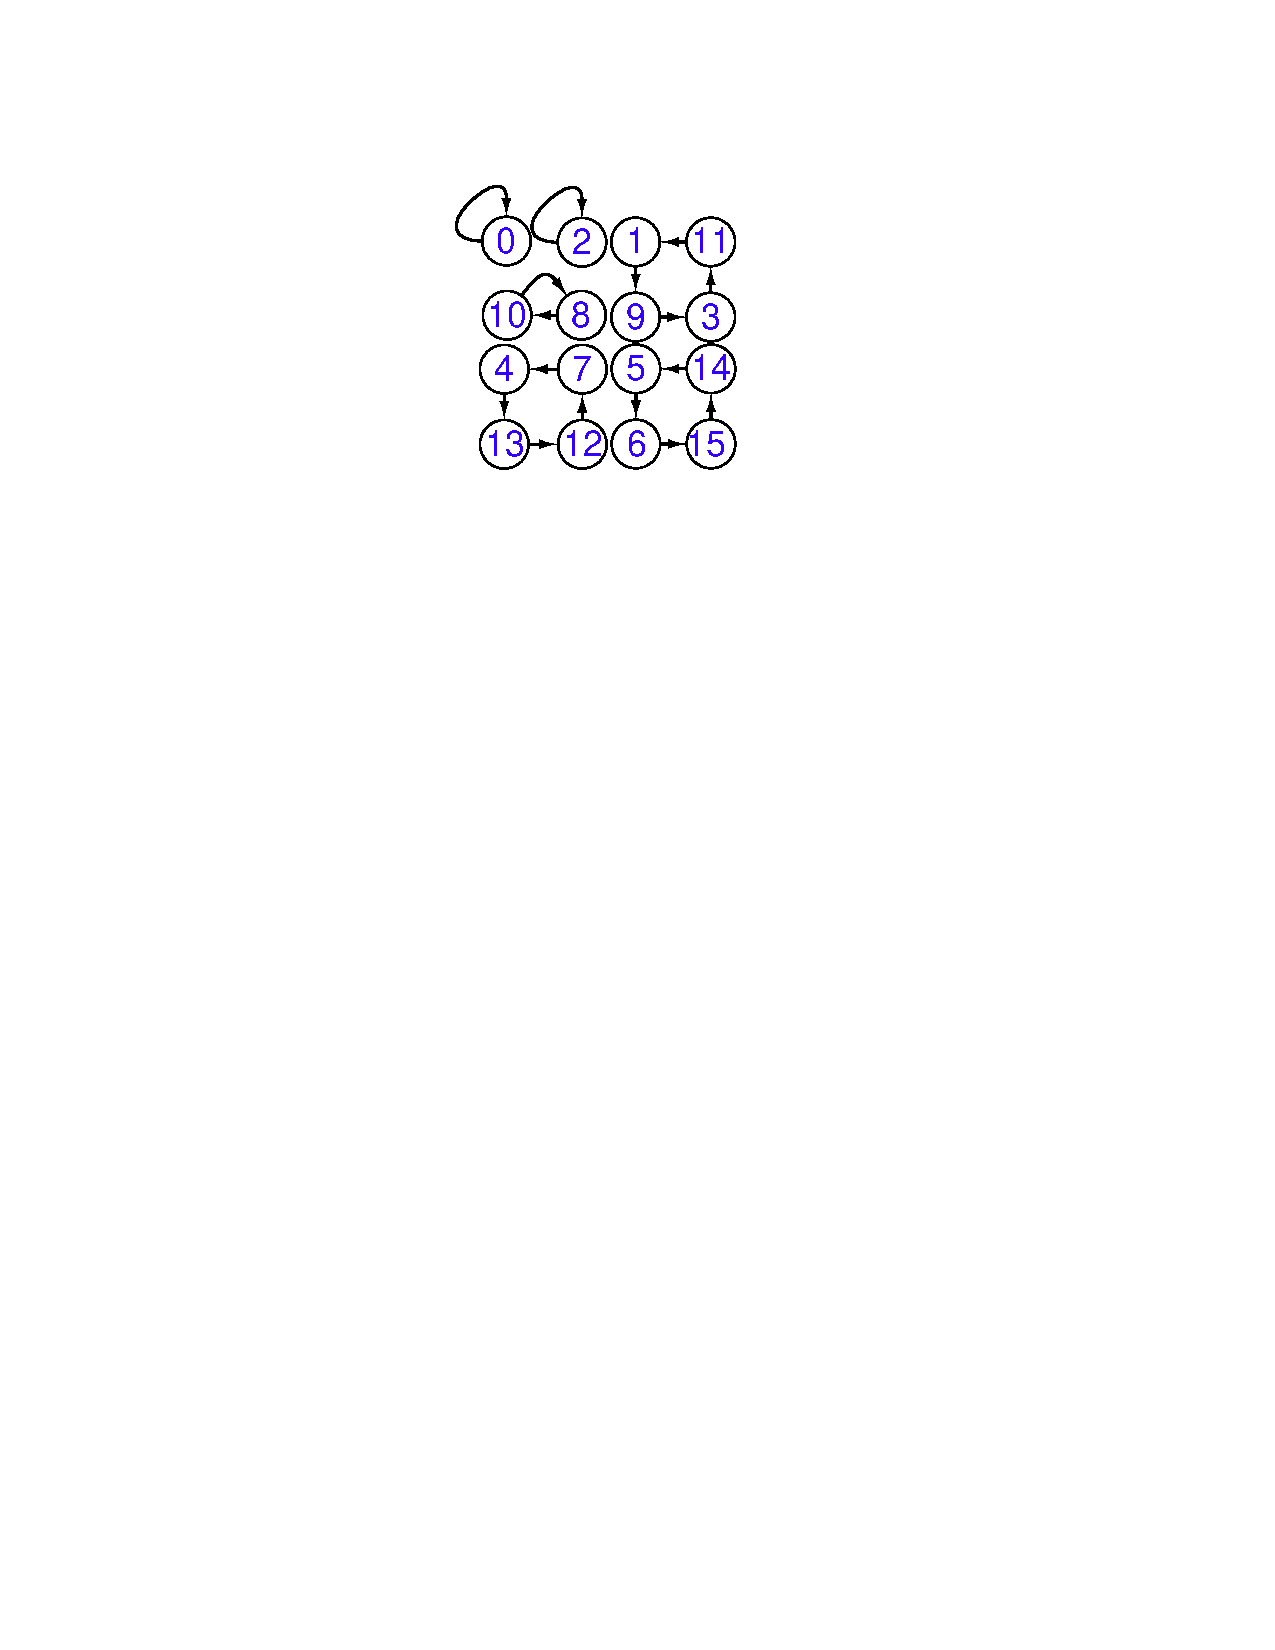
\includegraphics[width=\FourImW]{a1_b2_e2}
9)
\end{minipage}
\begin{minipage}[b]{\FourImW}
\centering
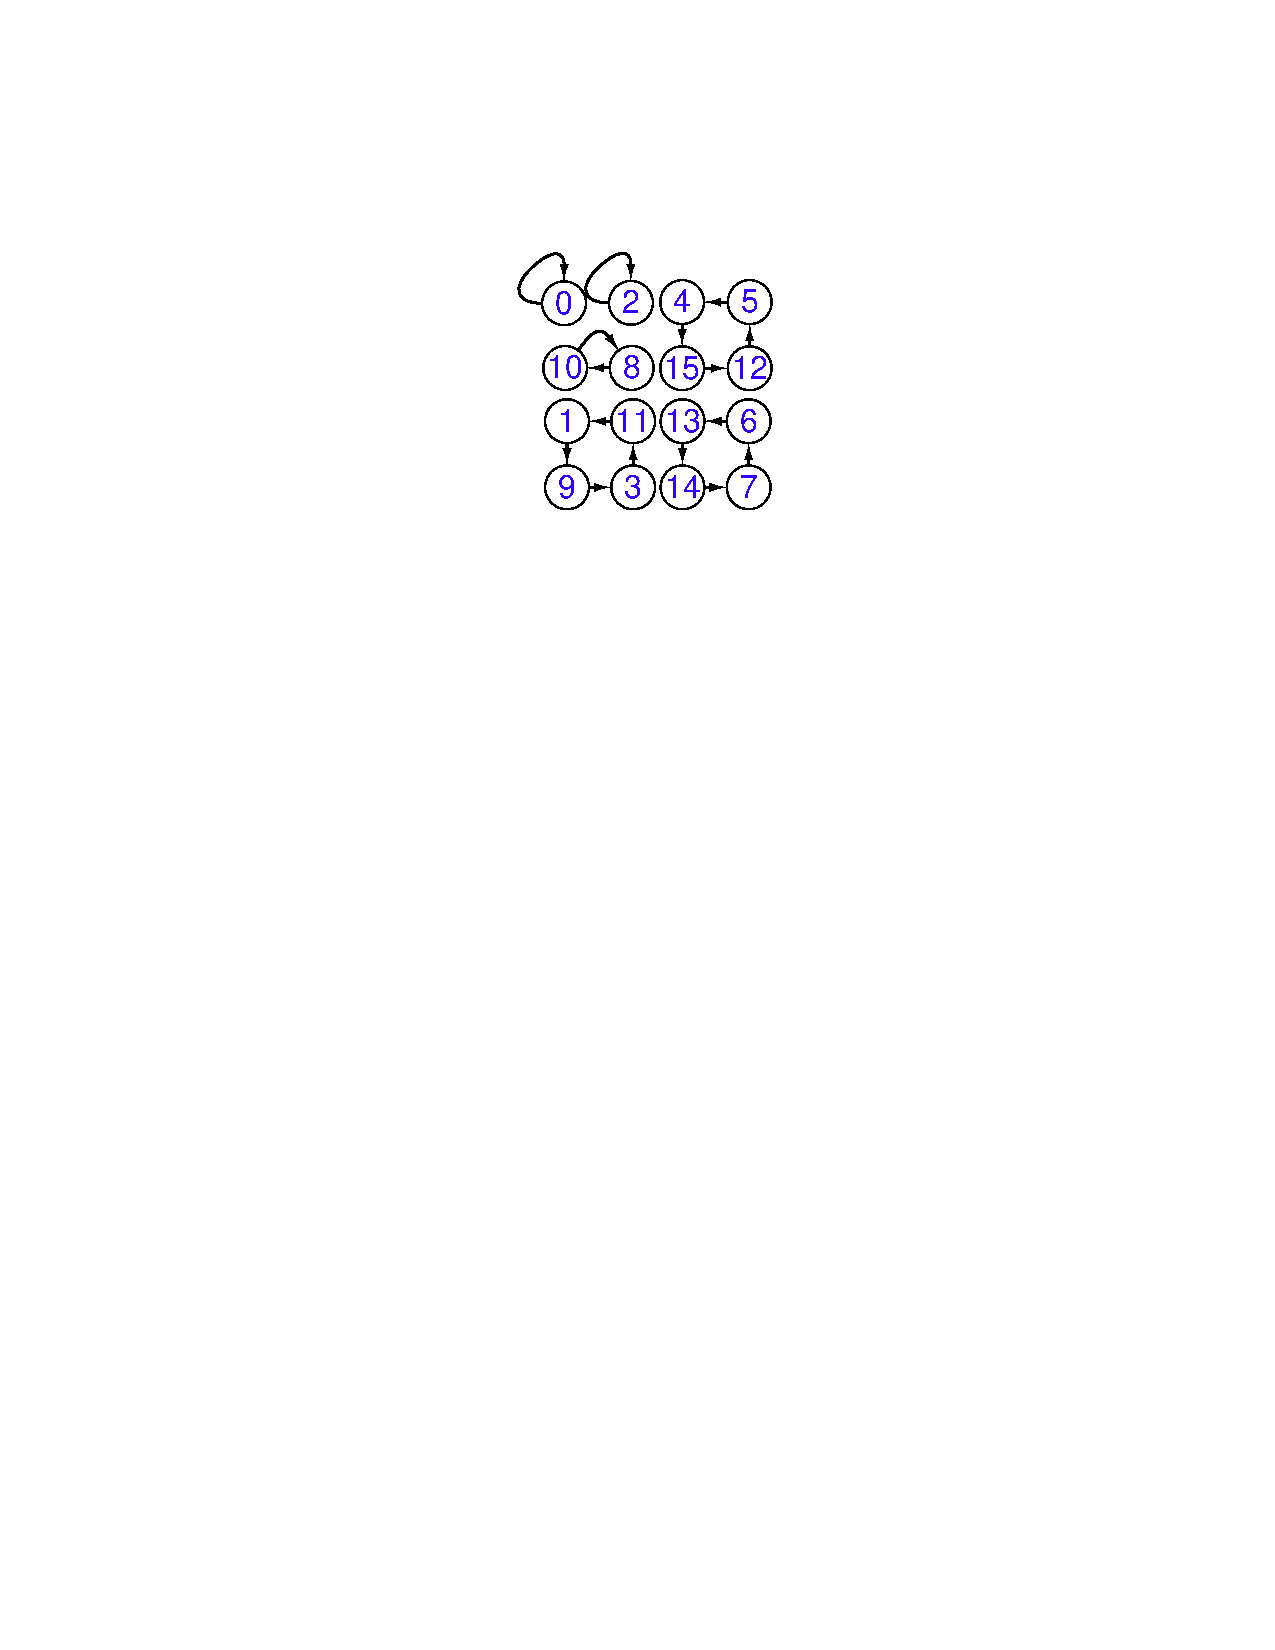
\includegraphics[width=\FourImW]{a3_b2_e2}
11)
\end{minipage}  \\
\begin{minipage}[b]{\FourImW}
\centering
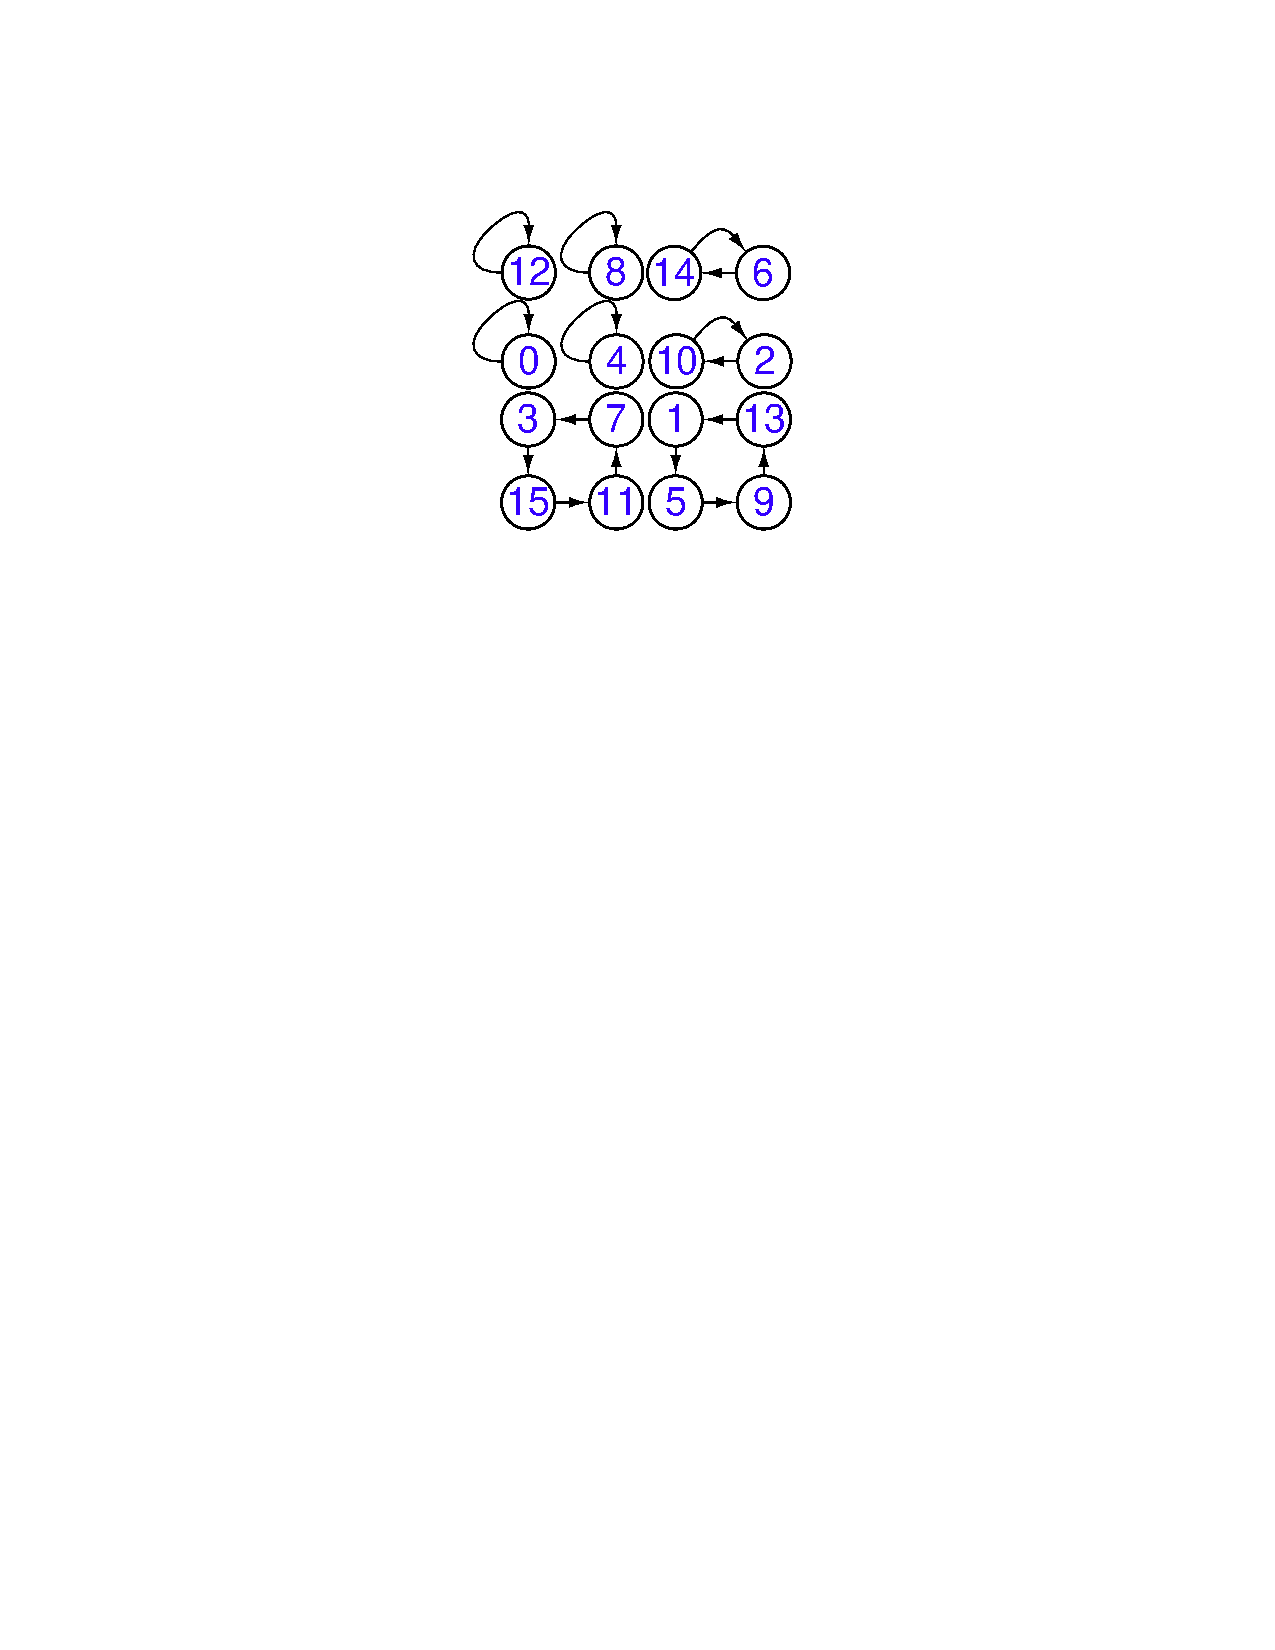
\includegraphics[width=\FourImW]{a0_b1_e2}
4)
\end{minipage}
\begin{minipage}[b]{\FourImW}
\centering
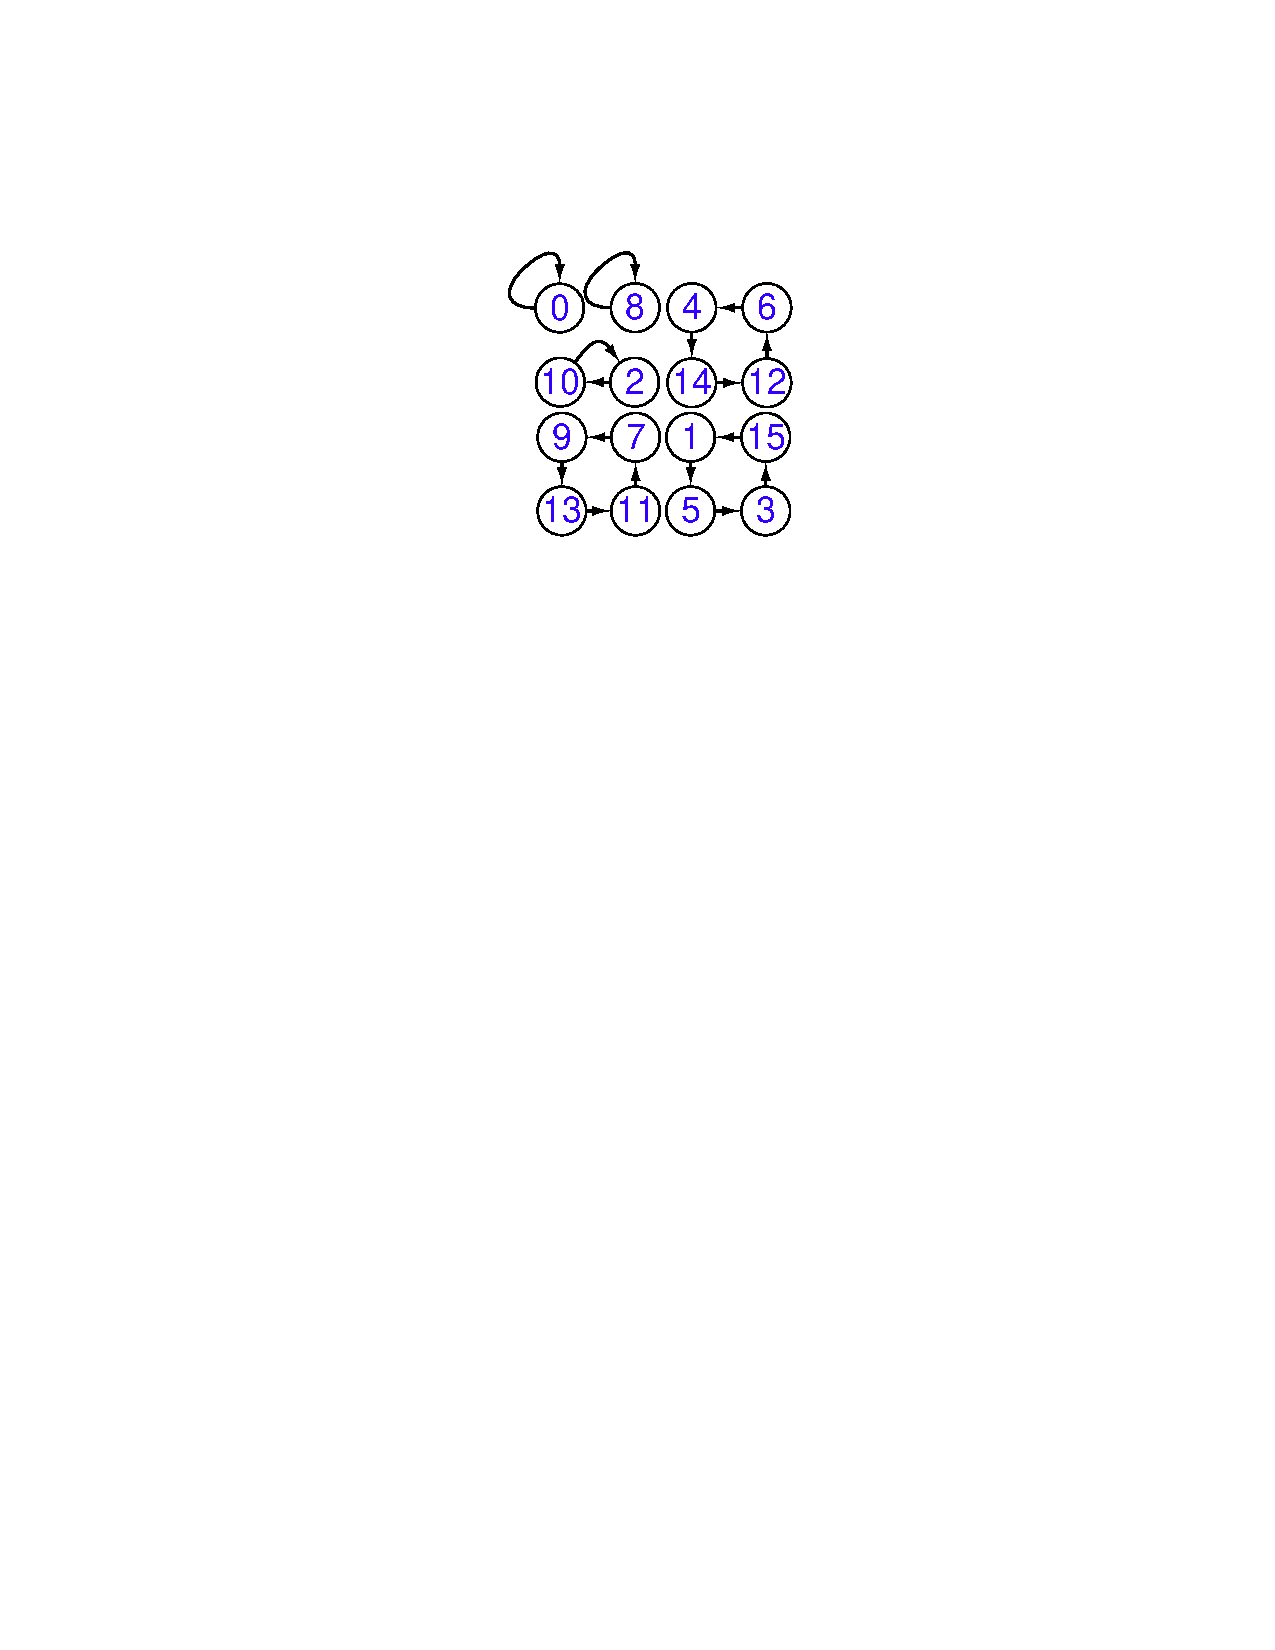
\includegraphics[width=\FourImW]{a2_b1_e2}
6)
\end{minipage}
\begin{minipage}[b]{\FourImW}
\centering
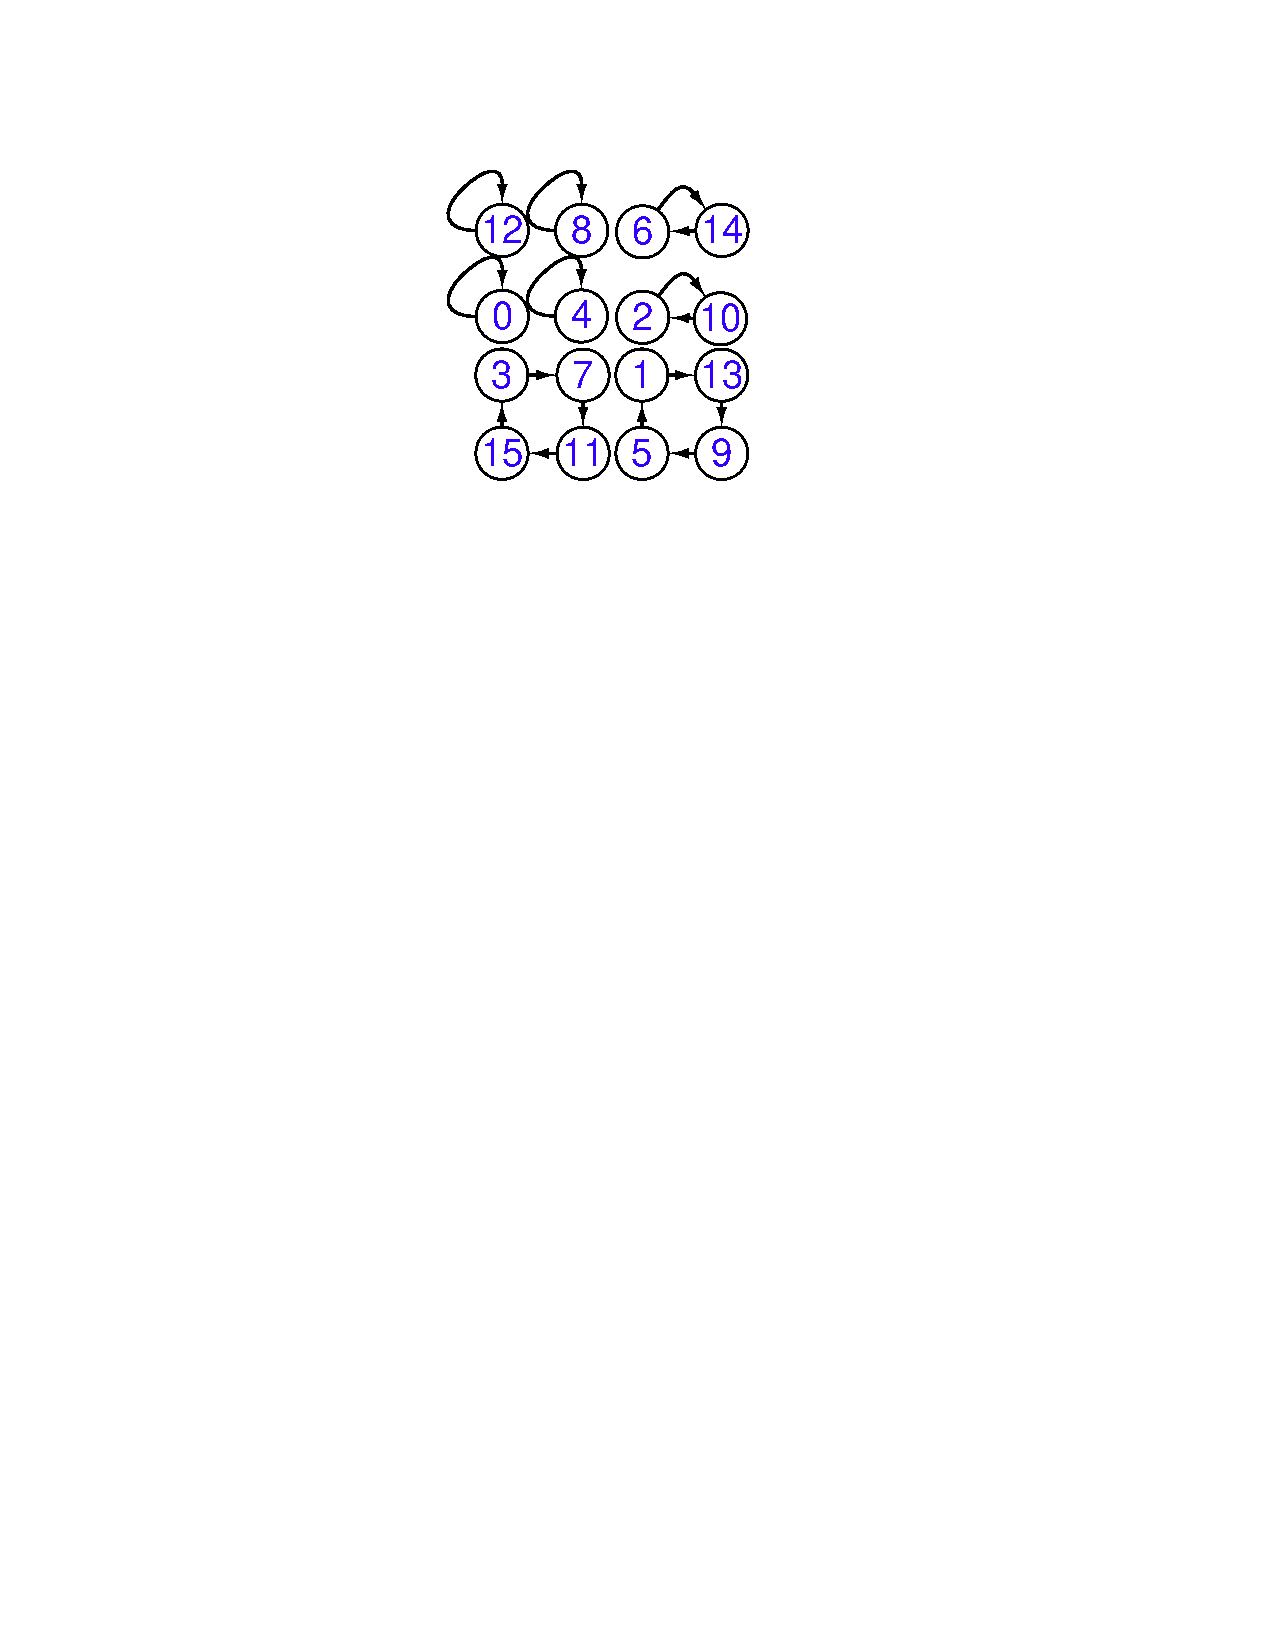
\includegraphics[width=\FourImW]{a0_b3_e2}
12)
\end{minipage}
\begin{minipage}[b]{\FourImW}
\centering
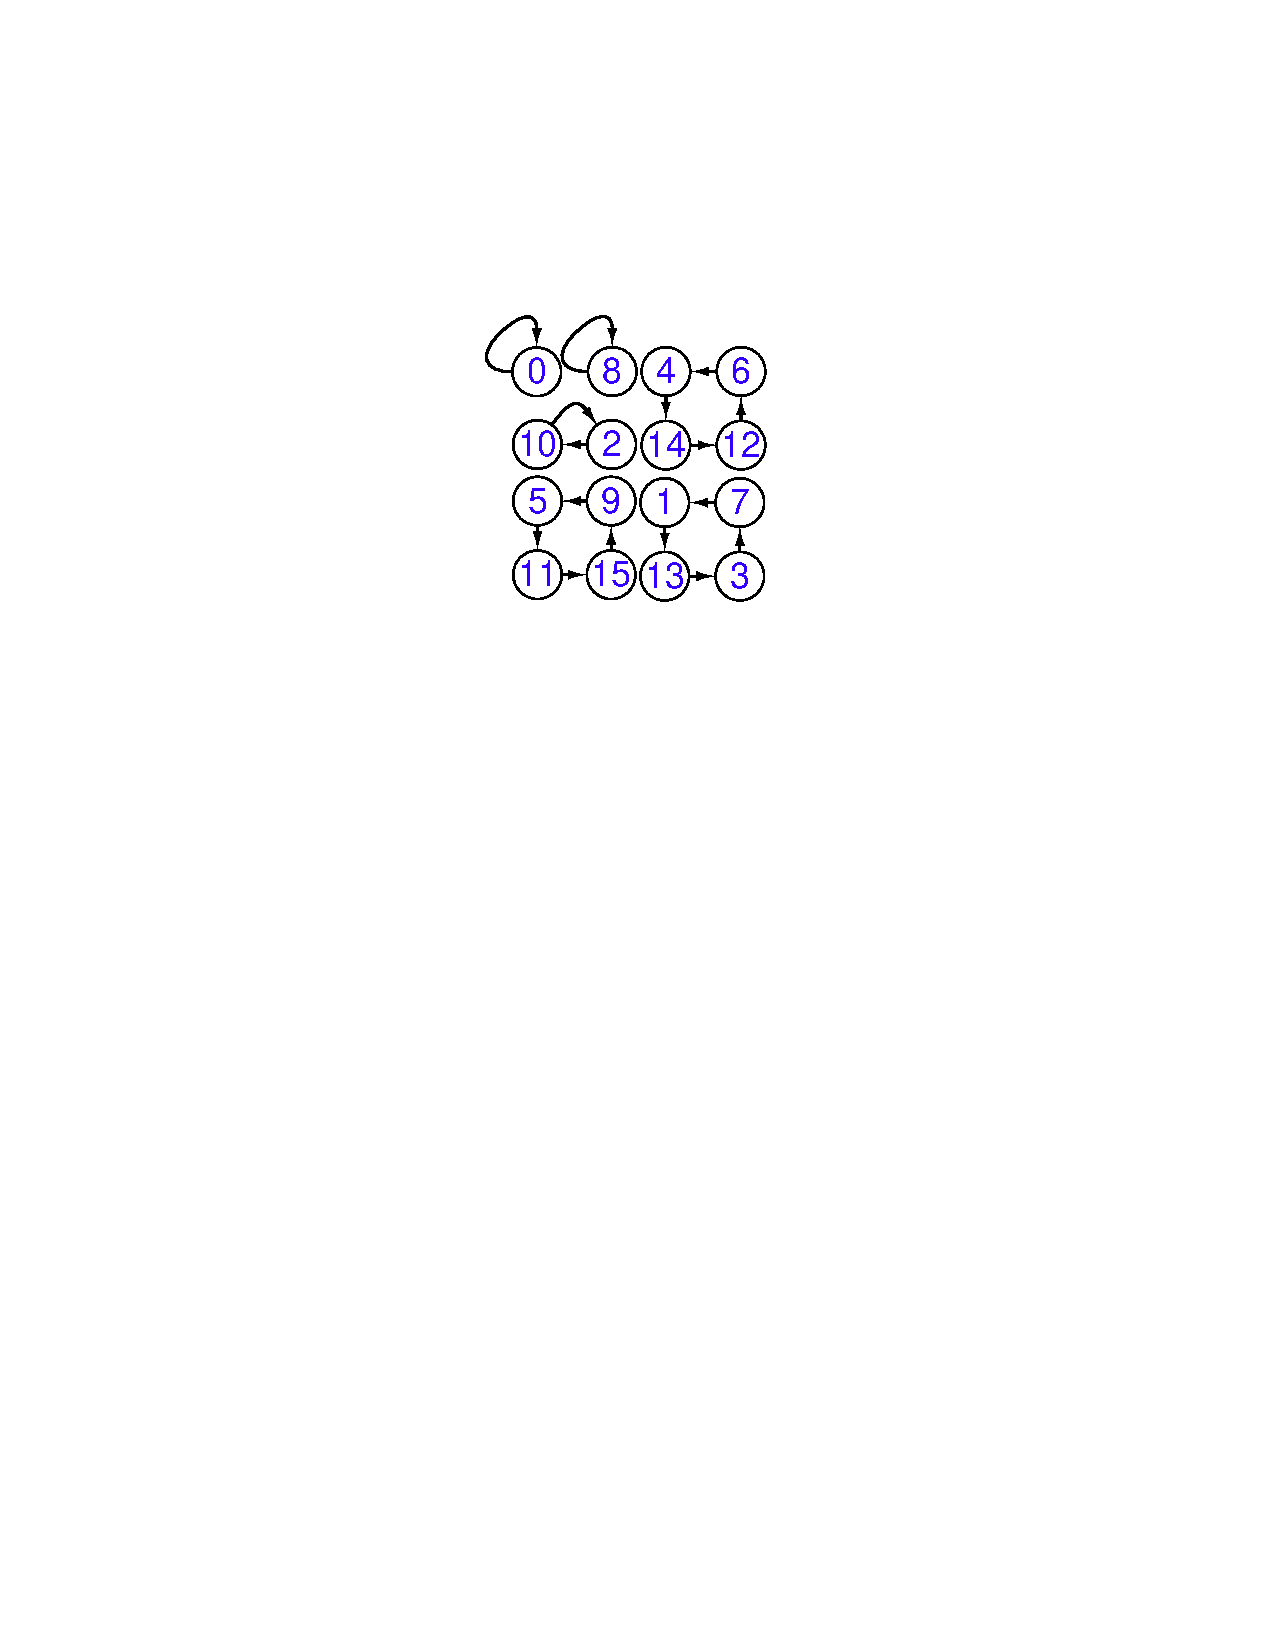
\includegraphics[width=\FourImW]{a2_b3_e2}
14)
\end{minipage}  \\
\begin{minipage}[b]{\FourImW}
\centering
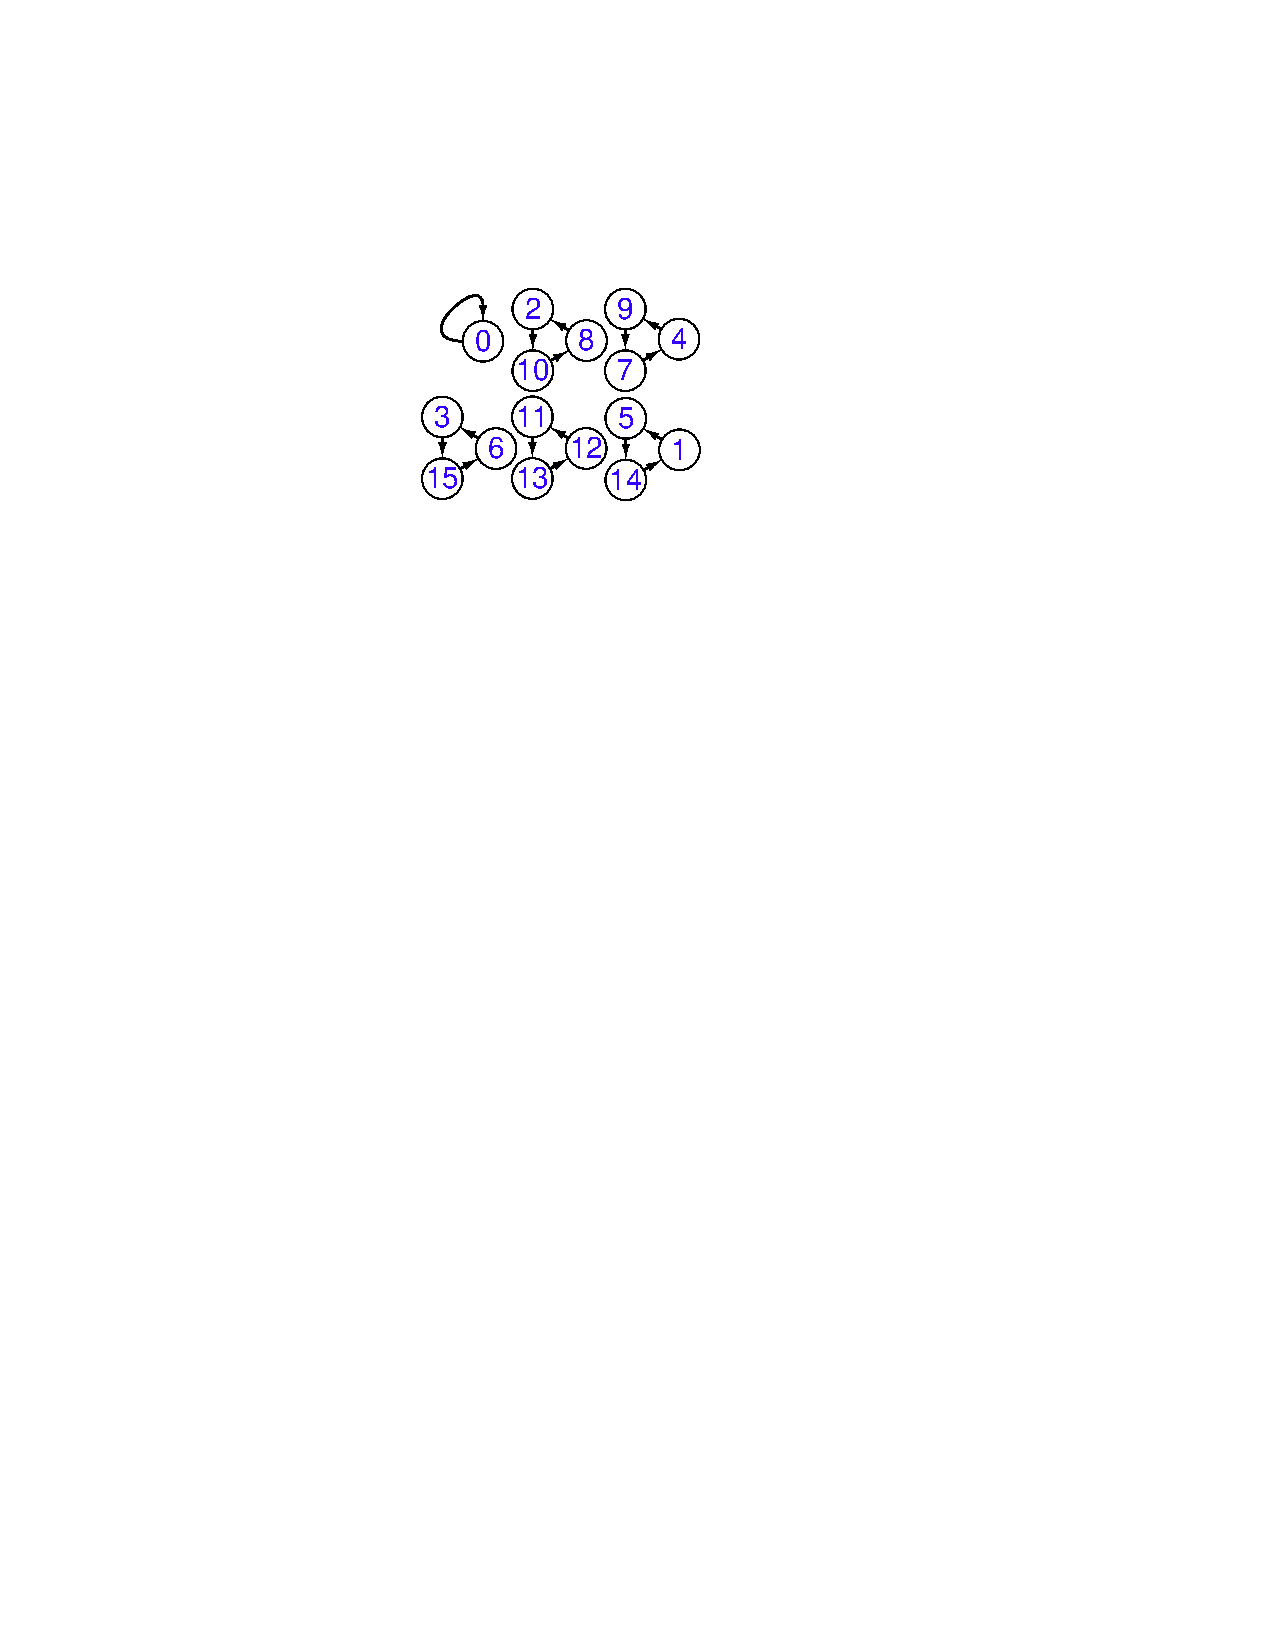
\includegraphics[width=\FourImW]{a1_b1_e2}
5)
\end{minipage}
\begin{minipage}[b]{\FourImW}
\centering
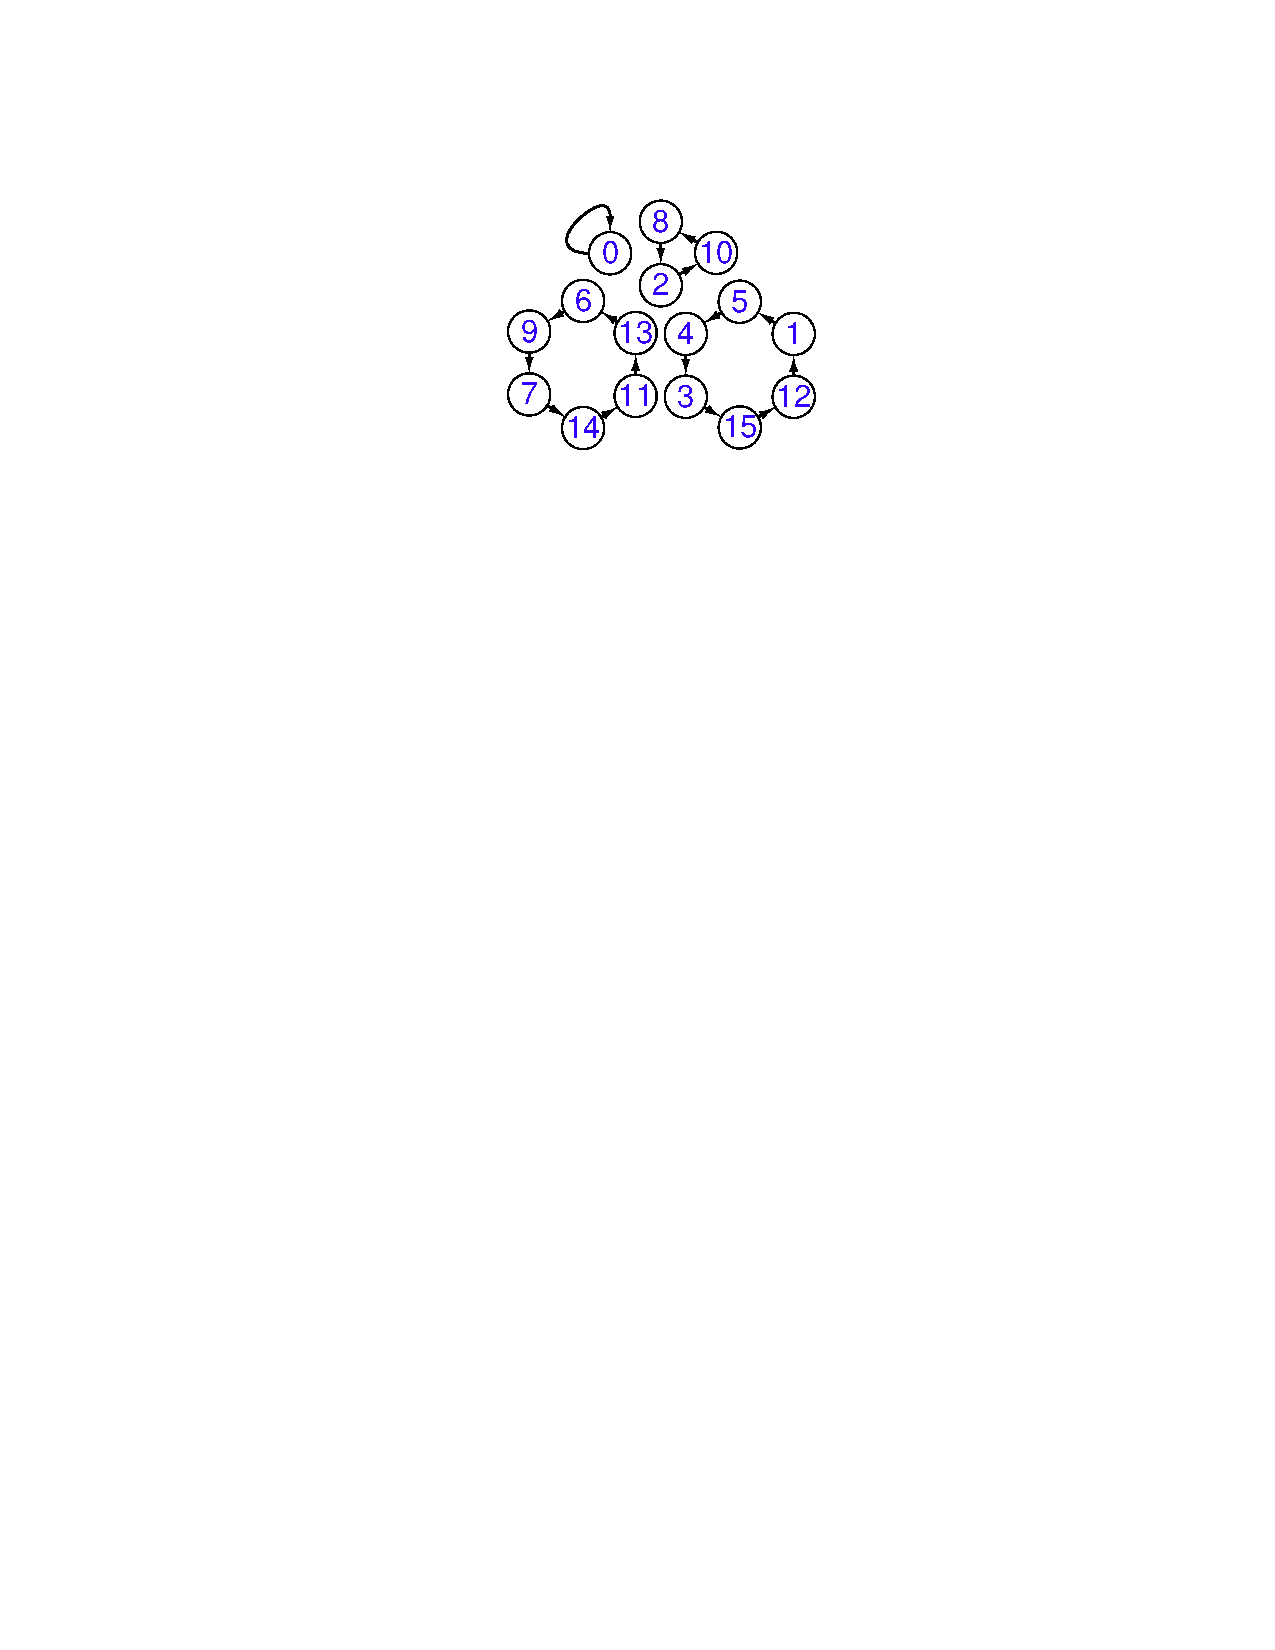
\includegraphics[width=\FourImW]{a3_b1_e2}
7)
\end{minipage}
\begin{minipage}[b]{\FourImW}
\centering
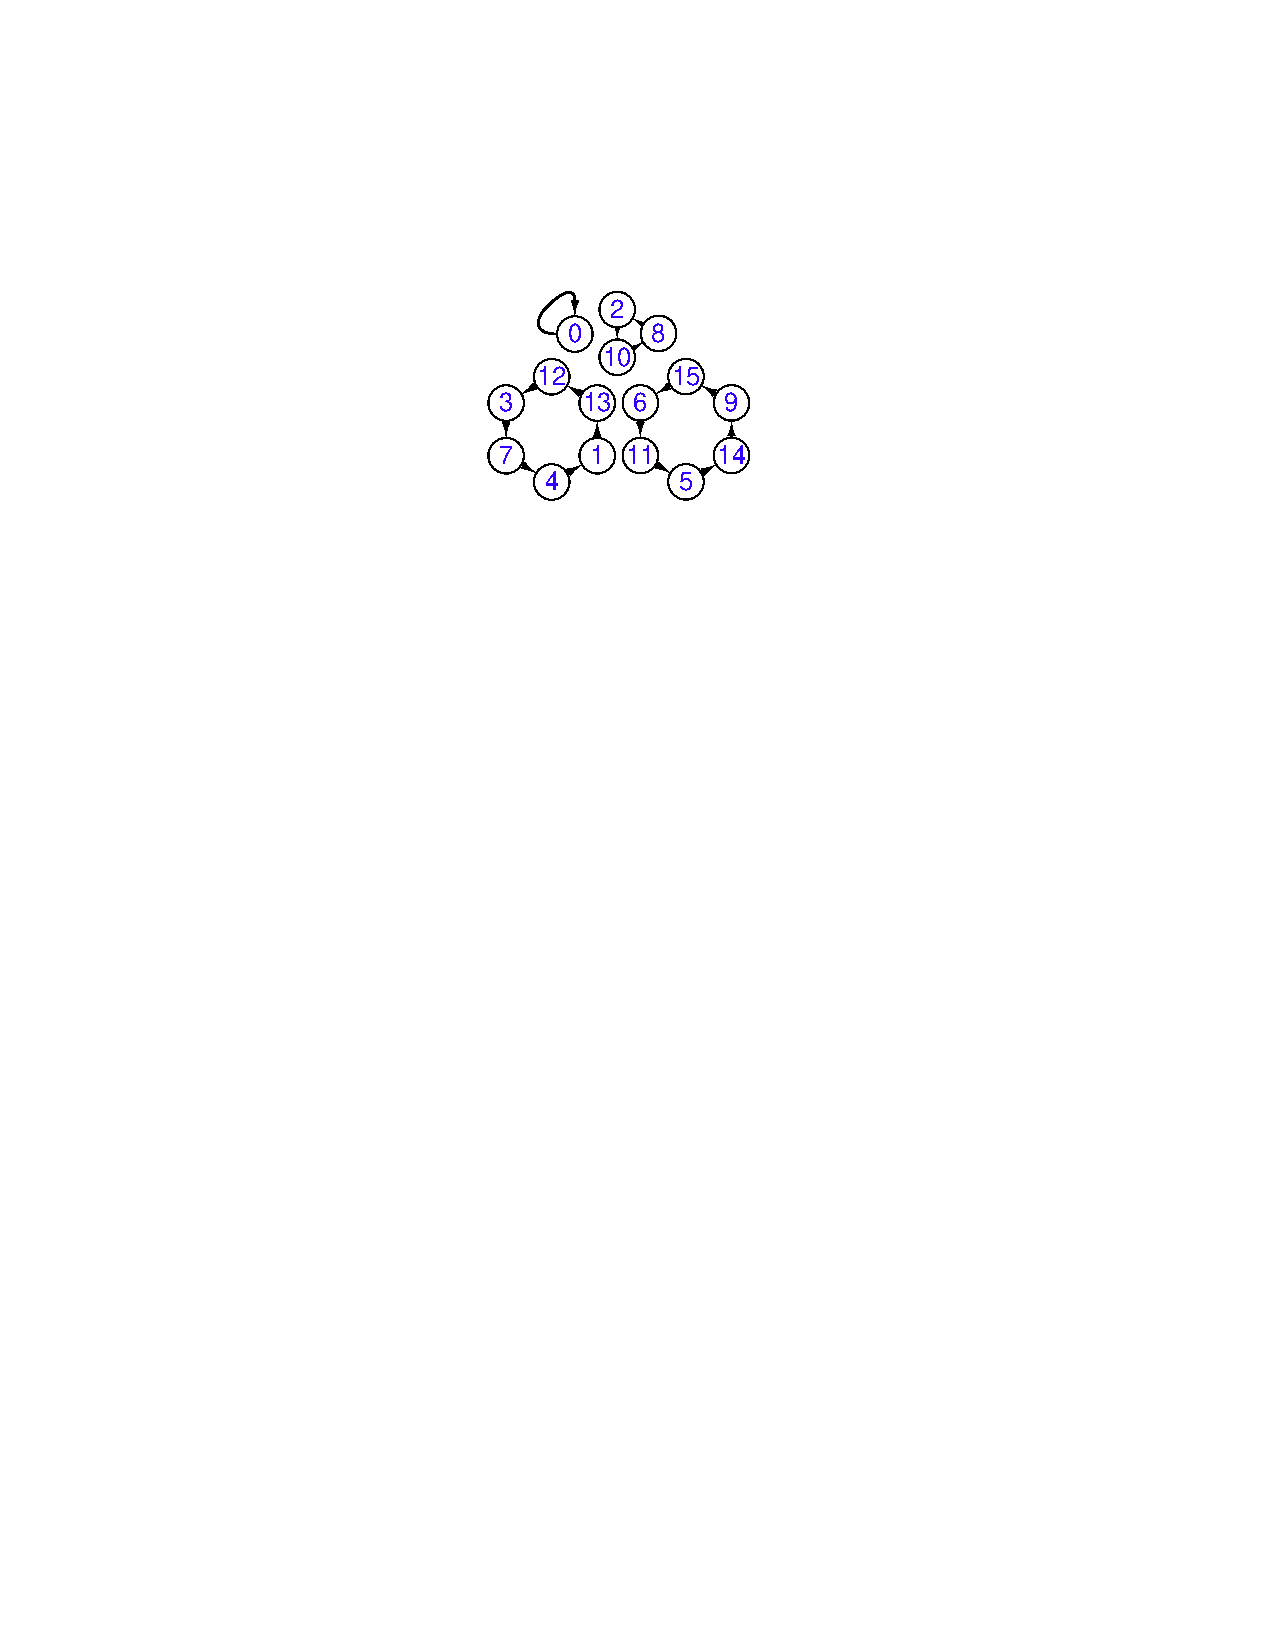
\includegraphics[width=\FourImW]{a1_b3_e2}
13)
\end{minipage}
\begin{minipage}[b]{\FourImW}
\centering
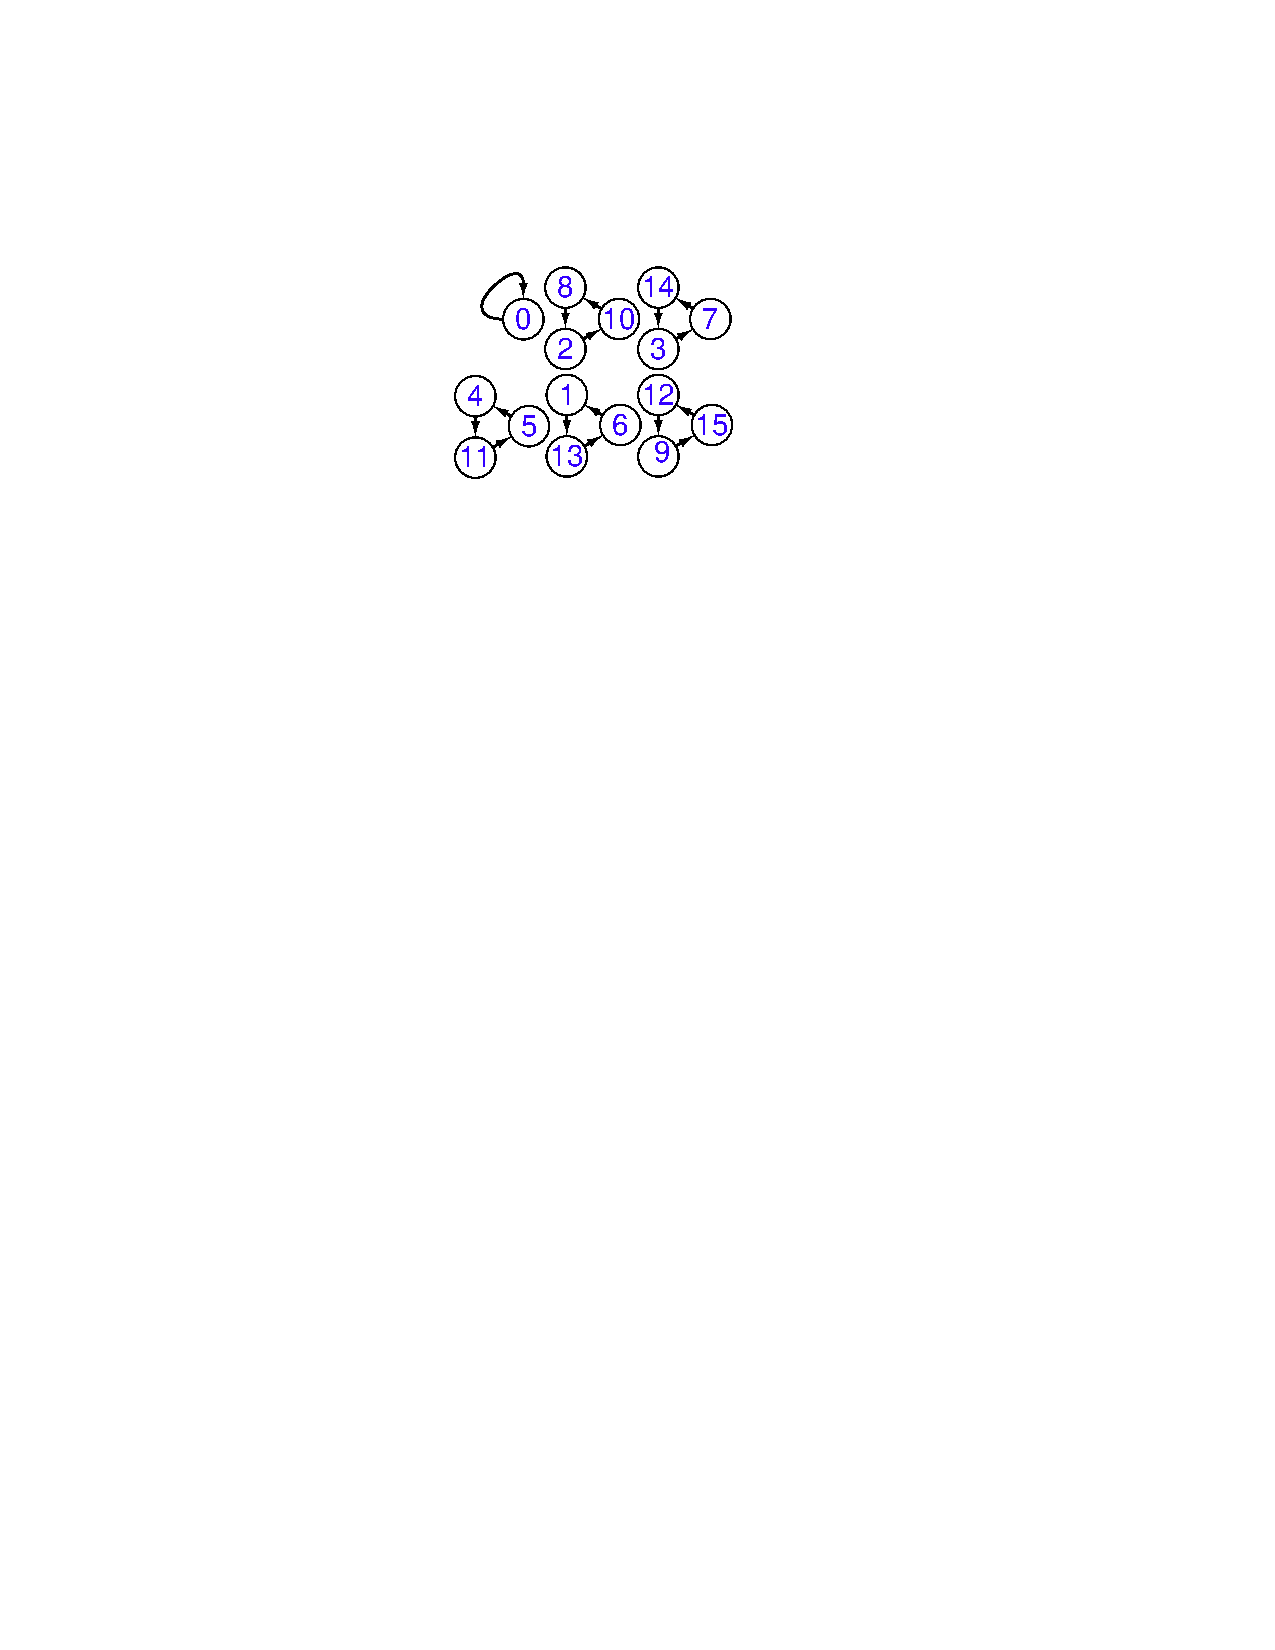
\includegraphics[width=\FourImW]{a3_b3_e2}
15)
\end{minipage}
\caption{$N=2^2$时,GDCM~(\ref{eq:ArnoldInteger})的所有可能状态映射网络,
第$i$个子图对应参数$(p, q)$满足$i=p\bmod 4+(q\bmod 4)\cdot 4$}
\label{Functionalgraphse1}
\end{figure}

\begin{Property}
给定$N$,GDCM~(\ref{eq:ArnoldInteger})状态映射网络的任何节点仅且只属于一个环,GDCM~(\ref{eq:ArnoldInteger})
将环上每个节点依次迭代映射到环上另一个节点。
\label{prop:onecycle}
\end{Property}
\begin{proof}
根据\cite[Theorem 5.1.1]{hall1959marshall}可知,集合$(0, 1, 2, \cdots, N^{2}-1)$关于GDCM~(\ref{eq:ArnoldInteger})
被划分为若干个不相交的子集,且每个子集构成一个环。\qedsymbol
\end{proof}

\begin{figure}[!htb]
\centering
\begin{minipage}{\BigTwoImW}
\centerline{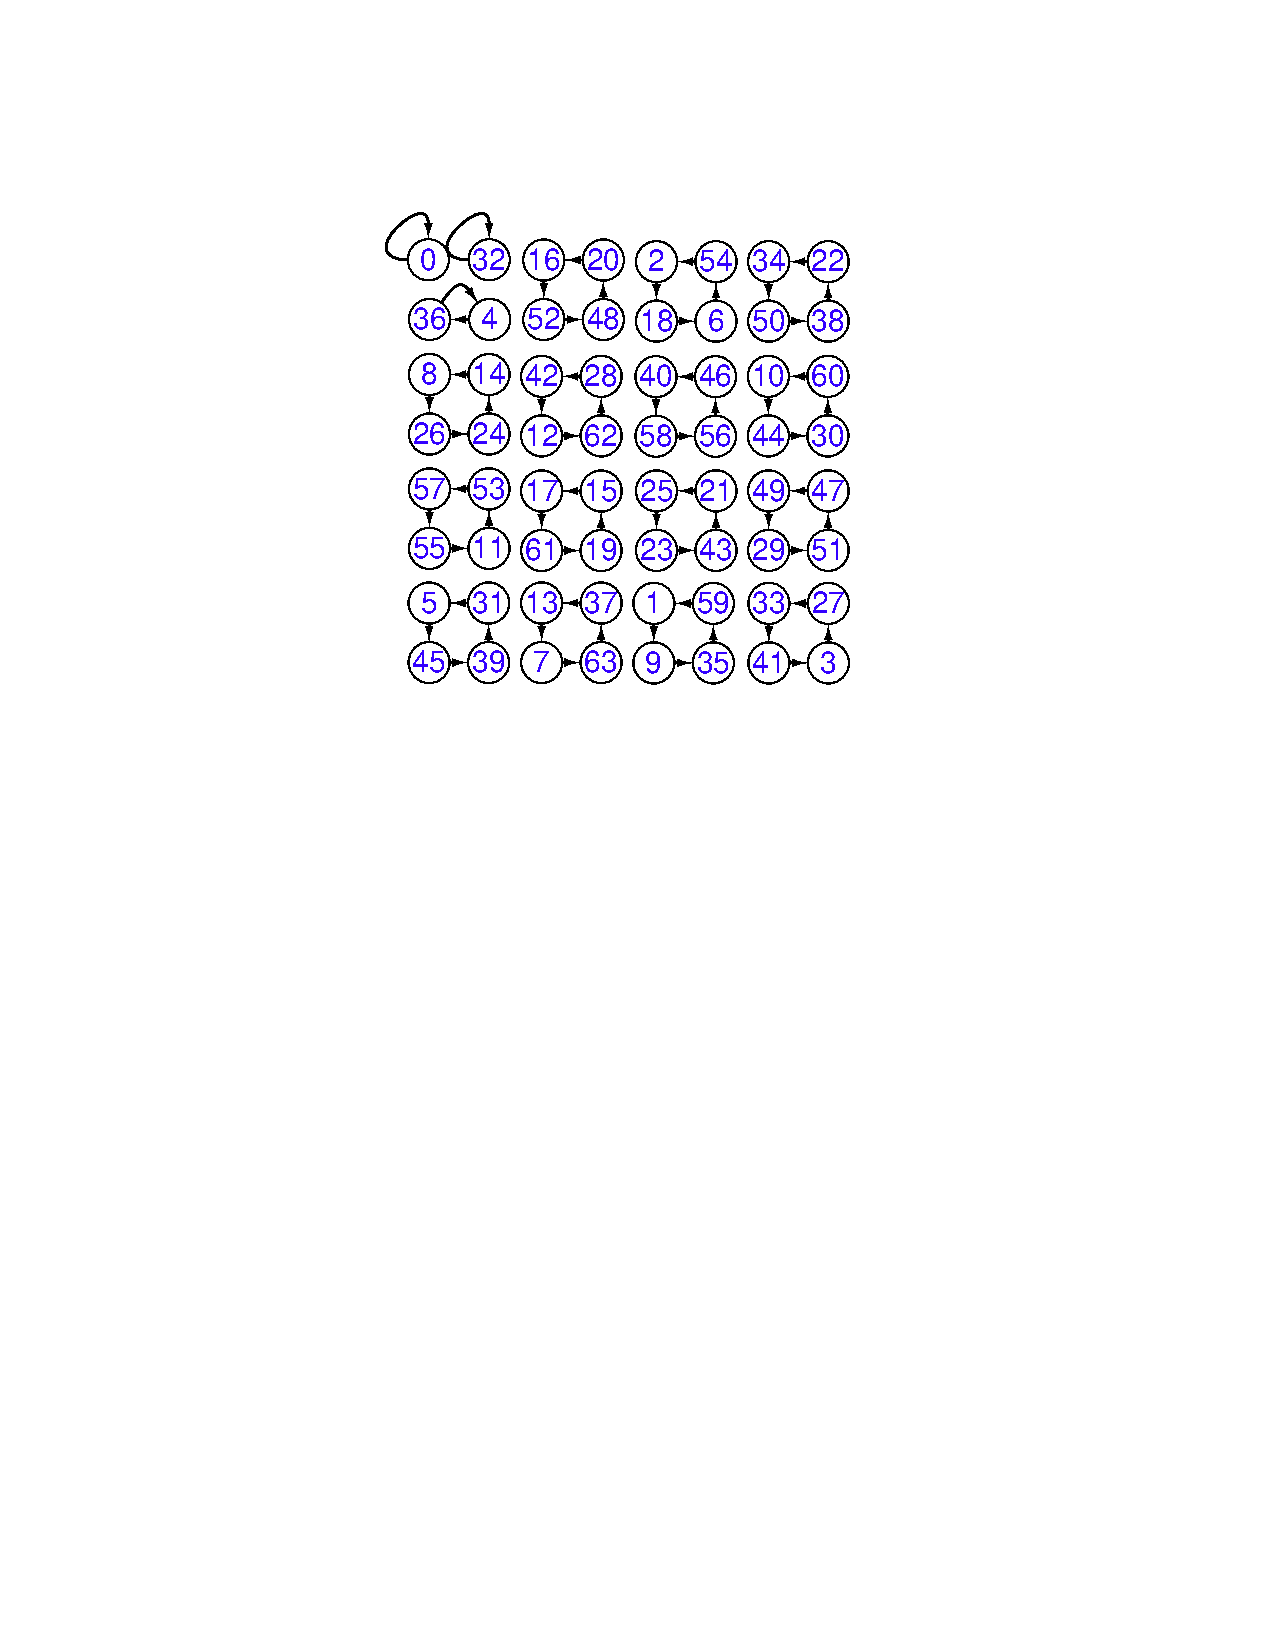
\includegraphics[width=\BigTwoImW]{a2_b1_e3}}
    \centerline{a)}
\end{minipage}\hspace{\figsep}
\begin{minipage}{\BigTwoImW}
 \centerline{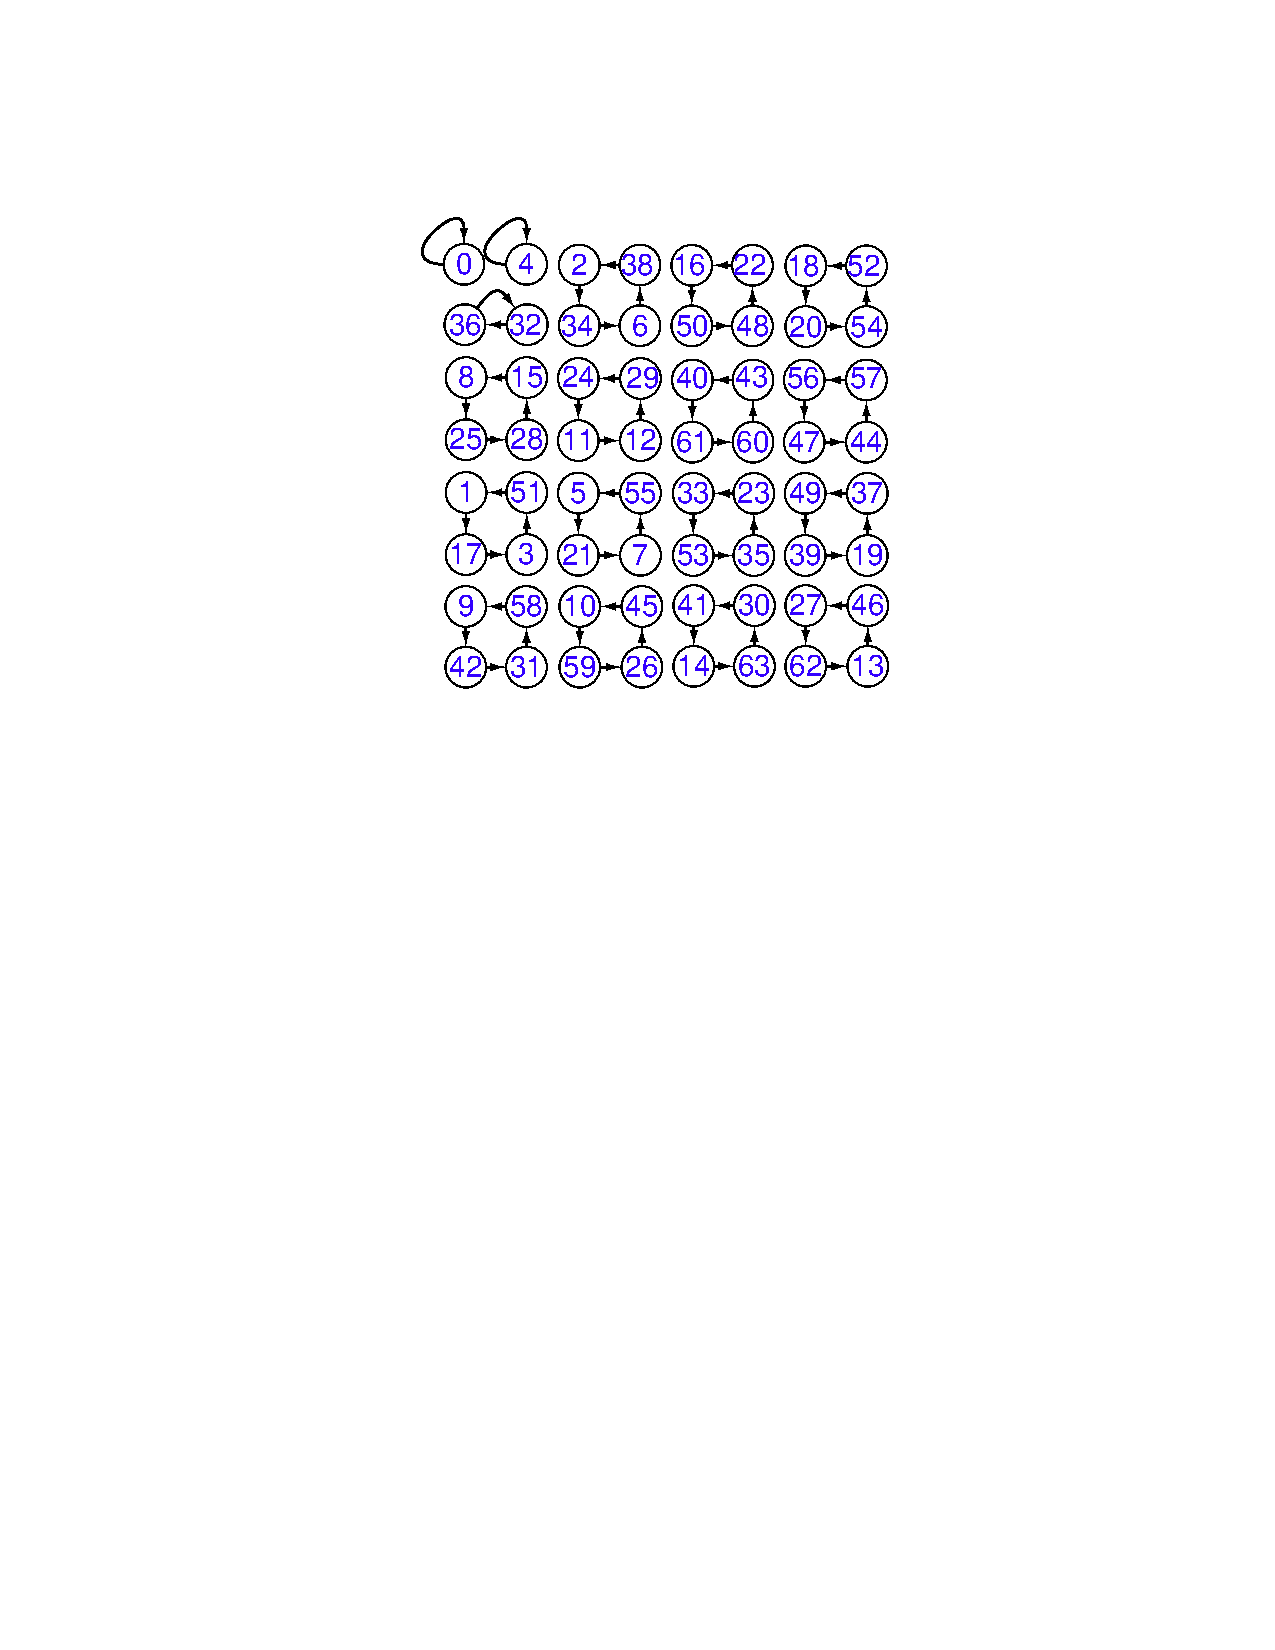
\includegraphics[width=\BigTwoImW]{a1_b2_e3}}
    \centerline{b)}
\end{minipage}
\caption{$N=2^3$时,GDCM~(\ref{eq:ArnoldInteger})的状态映射网络:
a) $(p, q)=(2, 1)$; b) $(p, q)=(1, 2)$}
\label{fig:Figure3d3c}
\end{figure}

GDCM~(\ref{eq:ArnoldInteger})的状态映射网络由许多短周期环构成,
图~\ref{fig:SMNcat} d)所示状态映射网络由16个周期为12的环,10个周期为6的环,1个周期为3的环和1个自环构成。
GDCM~(\ref{eq:ArnoldInteger})的周期为对应状态映射网络中所有可能周期的最小公倍数,
但参数$p,q$与GDCM~(\ref{eq:ArnoldInteger})周期之间的具体关系仍未可知\upcite{bohme2007security:Euler}。

$F_e$与$F_{e+1}$之间存在强相关关系,$F_e$中节点$z_{n, e}=x_{n, e}+y_{n, e}2^e$被演化为$F_{e+1}$中节点
\begin{eqnarray}
	z_{n, e+1} & = & (x_{n, e}+a_{n}2^e) + (y_{n, e}+b_{n}2^e) 2^{e+1} \nonumber\\
	           & = & z_{n, e}+(a_{n}2^e+y_{n, e}2^e+b_{n}2^{2e+1} ),
\label{eq:evoluteNumber}	
\end{eqnarray}
其中$a_{n}, b_{n}\in \{0, 1\}$。
性质~\ref{Property:evolution}揭示了$F_e$中节点$z_{n, e}$的迭代节点与$F_{e+1}$中对应节点之间的演化规律,
性质~\ref{Prop:cycleExpan}揭示了$F_e$中给定环与$F_{e+1}$中对应环之间的具体关系。

\begin{figure*}[!htb]
\centering
\begin{minipage}{0.95\BigOneImW}
\centering
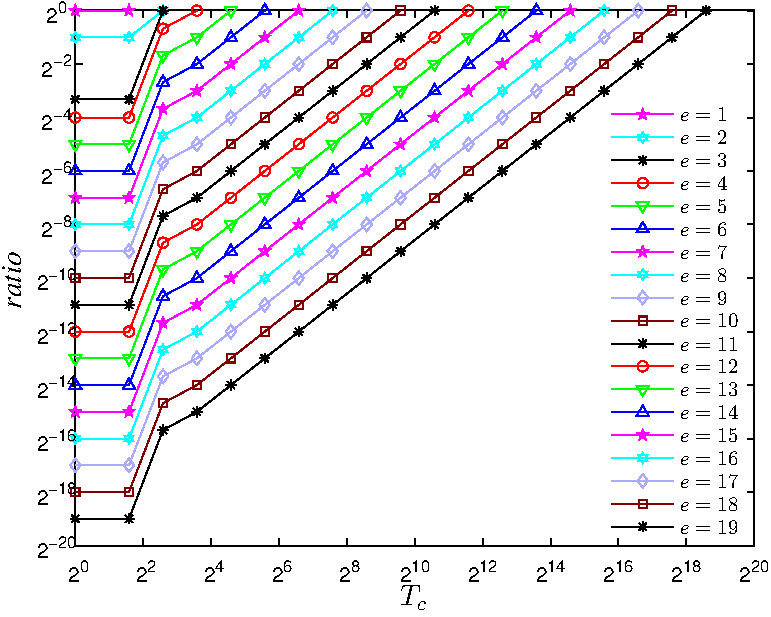
\includegraphics[width=0.95\BigOneImW]{period_cat_e1_19_a5b7}
a)
\end{minipage} \hspace{1mm}
\begin{minipage}{0.95\BigOneImW}
\centering
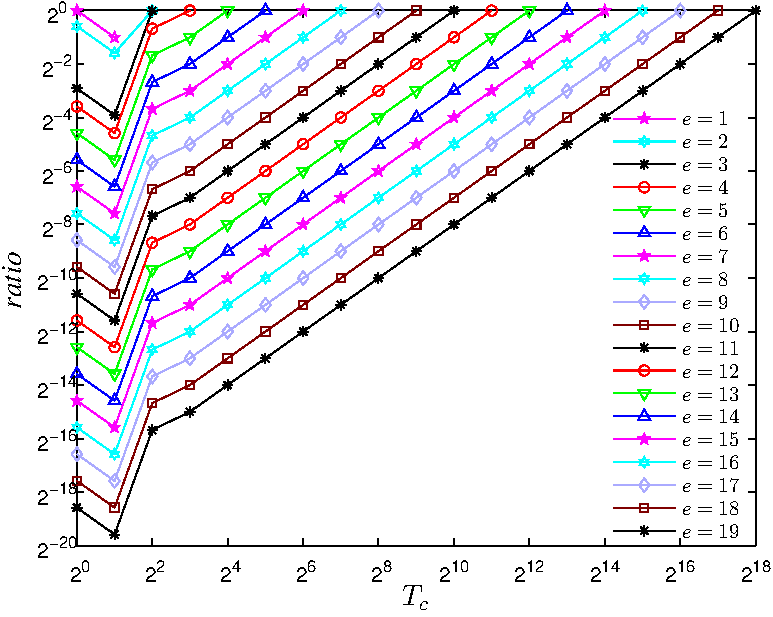
\includegraphics[width=0.95\BigOneImW]{period_cat_e1_19_a6b7}
b)
\end{minipage}\\
\begin{minipage}{0.95\BigOneImW}
\centering
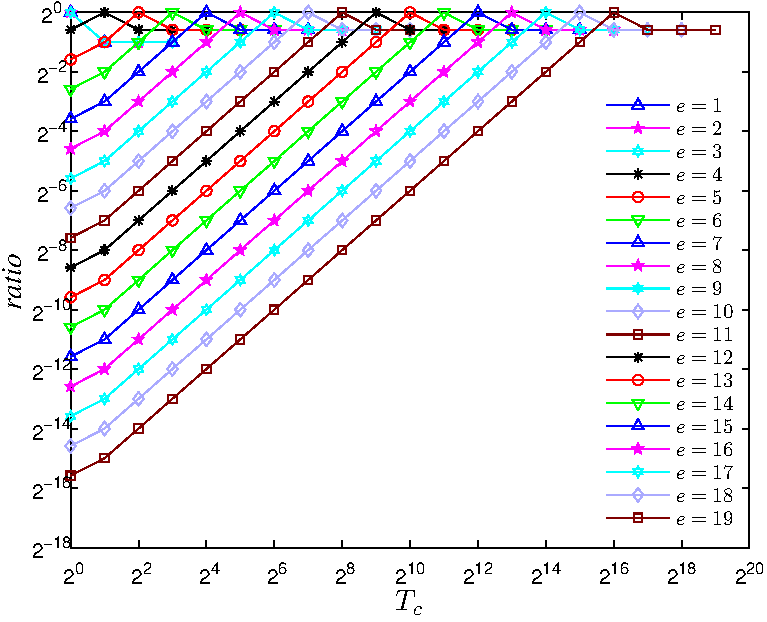
\includegraphics[width=0.95\BigOneImW]{period_cat_e1_19_a7b8}
c)
\end{minipage} \hspace{1mm}
\begin{minipage}{0.95\BigOneImW}
\centering
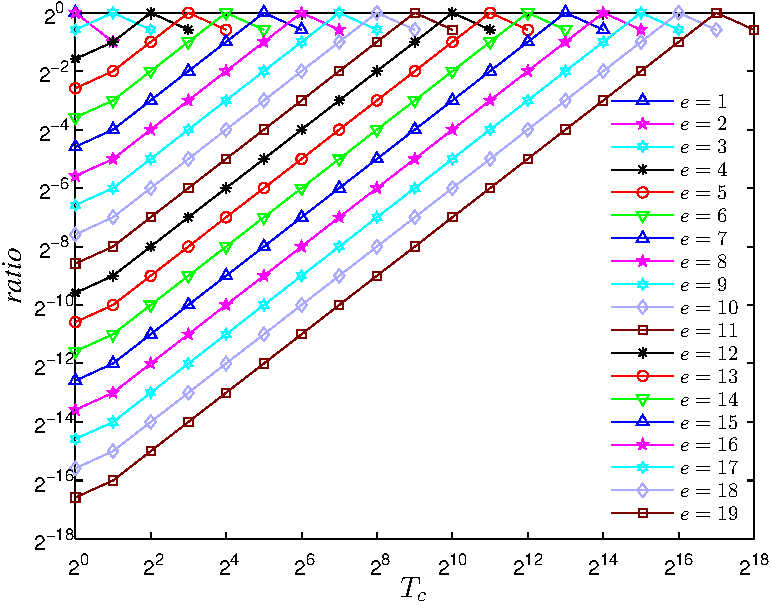
\includegraphics[width=0.95\BigOneImW]{period_cat_e1_19_a12b14}
d)
\end{minipage}
\caption{有限域$\mathbb{Z}_{2^e}$上GDCM~(\ref{eq:ArnoldInteger})的环分布,其中$e=1\sim 19$:
a) $(p, q)=(5, 7)$; b) $(p, q)=(6, 7)$; c) $(p, q)=(7, 8)$; b) $(p, q)=(12, 14)$}
\label{fig:perioddistributionab}
\end{figure*}

\begin{Property}
若$N=2^e$时GDCM~(\ref{eq:ArnoldInteger})的输入与$N=2^{e+1}$时GDCM~(\ref{eq:ArnoldInteger})的输入
满足关系
\begin{equation}
\begin{bmatrix}
		x_{n, e+1}-x_{n, e} \\
		y_{n, e+1}-y_{n, e}
	\end{bmatrix}
=
\begin{bmatrix}
		a_n \\
		b_n
	\end{bmatrix} \cdot 2^e,
\label{eq:condition}
\end{equation}
则有
\begin{equation}
	\begin{bmatrix}
		a_{n+1}\\
		b_{n+1}
	\end{bmatrix}
	=
	\left[\begin{bmatrix}
		1 & p    \\
		q & 1+p\cdot q
	\end{bmatrix}\cdot
	\begin{bmatrix}
		a_n  \\
		b_n
	\end{bmatrix}+
	\begin{bmatrix}
		k_x \\
		k_y
	\end{bmatrix}\right] \bmod 2,
		\label{eq:kxky}
\end{equation}
$a_n, b_n\in \{0, 1\}$,$k_x=\lfloor k'_x/2^e\rfloor$, $k_y=\lfloor k'_y/2^e\rfloor$,且

\begin{equation}
	\begin{bmatrix}
		k'_x \\
		k'_y
	\end{bmatrix}
	=
	\begin{bmatrix}
		1 & p    \\
		q & 1+p\cdot q
	\end{bmatrix}\cdot
	\begin{bmatrix}
		x_{n, e} \\
		y_{n, e}
	\end{bmatrix}.
\label{eq:k2xk2y}
\end{equation}
\label{Property:evolution}
\end{Property}
\setlength{\arraycolsep}{2pt}
\begin{proof}
根据$N=2^e$时GDCM~(\ref{eq:ArnoldInteger})与$N=2^{e+1}$时GDCM~(\ref{eq:ArnoldInteger})之间的线性关系,可得
\begin{eqnarray}
    \begin{bmatrix}
		x_{n+1, e+1}-x_{n+1, e} \\
		y_{n+1, e+1}-x_{n+1, e}
	\end{bmatrix}
& \equiv &
	\begin{bmatrix}
		1 & p    \\
		q & 1+p\cdot q
	\end{bmatrix}
	\begin{bmatrix}
		x_{n, e+1}-x_{n, e} \\
		y_{n, e+1}-y_{n, e}
	\end{bmatrix}
+2^e
    \begin{bmatrix}
		k_x \\
		k_y
	\end{bmatrix}
\Mod{2^{e+1}}.
\label{eq:ArnoldIntegerdiff}
\end{eqnarray}
\begin{equation}
k\cdot a\equiv k\cdot a'\Mod{m}
\end{equation}
当且仅当
\begin{equation}
a\equiv a'\left(\Mod{\frac{m}{\gcd(m, k)}}\right),\ a_{n+1, e}, b_{n+1, e}\in \{0, 1\}.
\label{eq:gcd_mk}
\end{equation}
将条件~(\ref{eq:condition})代入余式~(\ref{eq:ArnoldIntegerdiff}),根据~(\ref{eq:gcd_mk})式,余式两边和模数同除以$2^e$即可证明上述性质。\qedsymbol
\end{proof}

\begin{figure*}[!htb]
\centering
\begin{minipage}{0.95\BigOneImW}
\centering
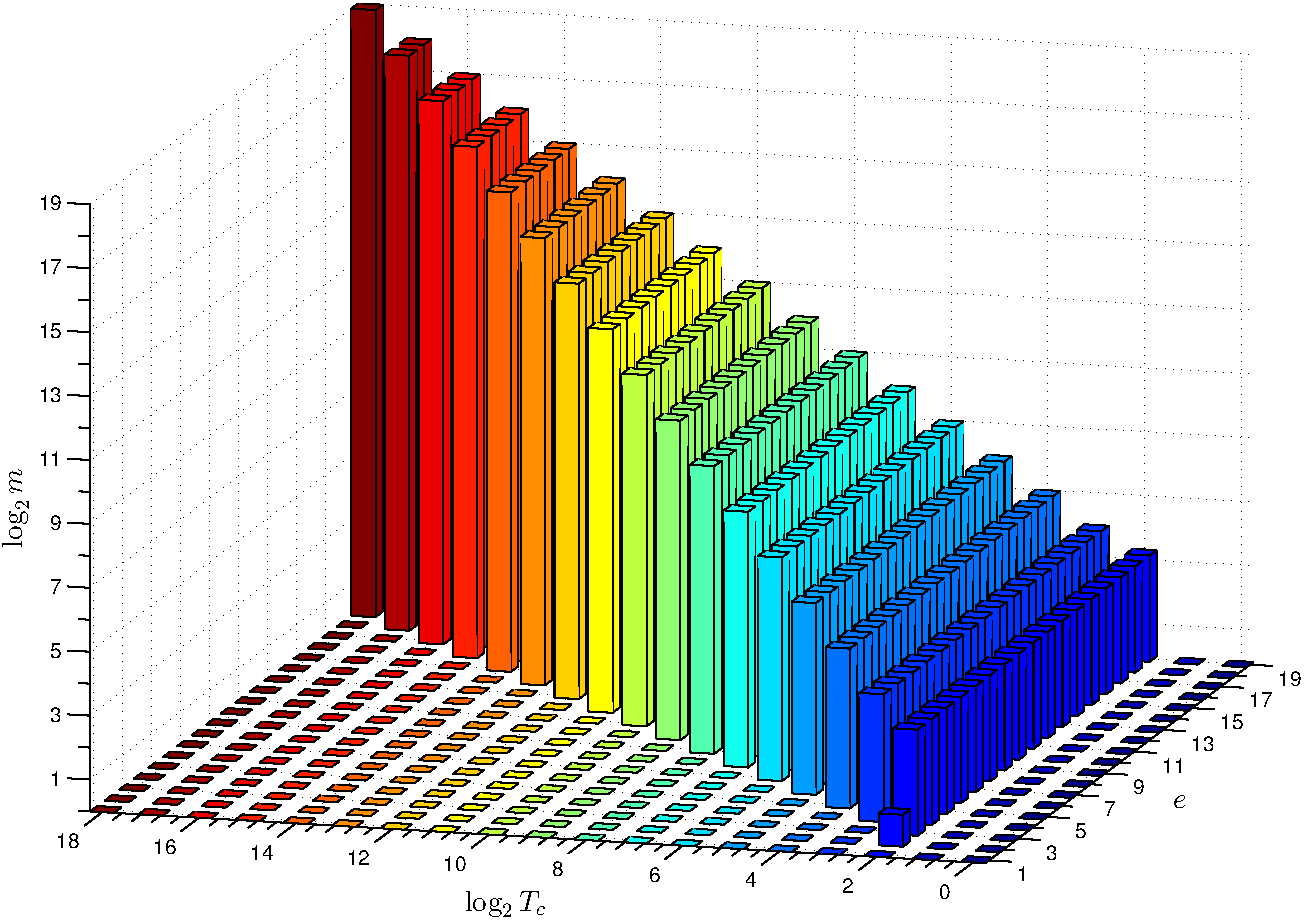
\includegraphics[width=0.95\BigOneImW]{e_T_m_3D_hist_a5b7}
a)
\end{minipage} \hspace{1mm}
\begin{minipage}{0.95\BigOneImW}
\centering
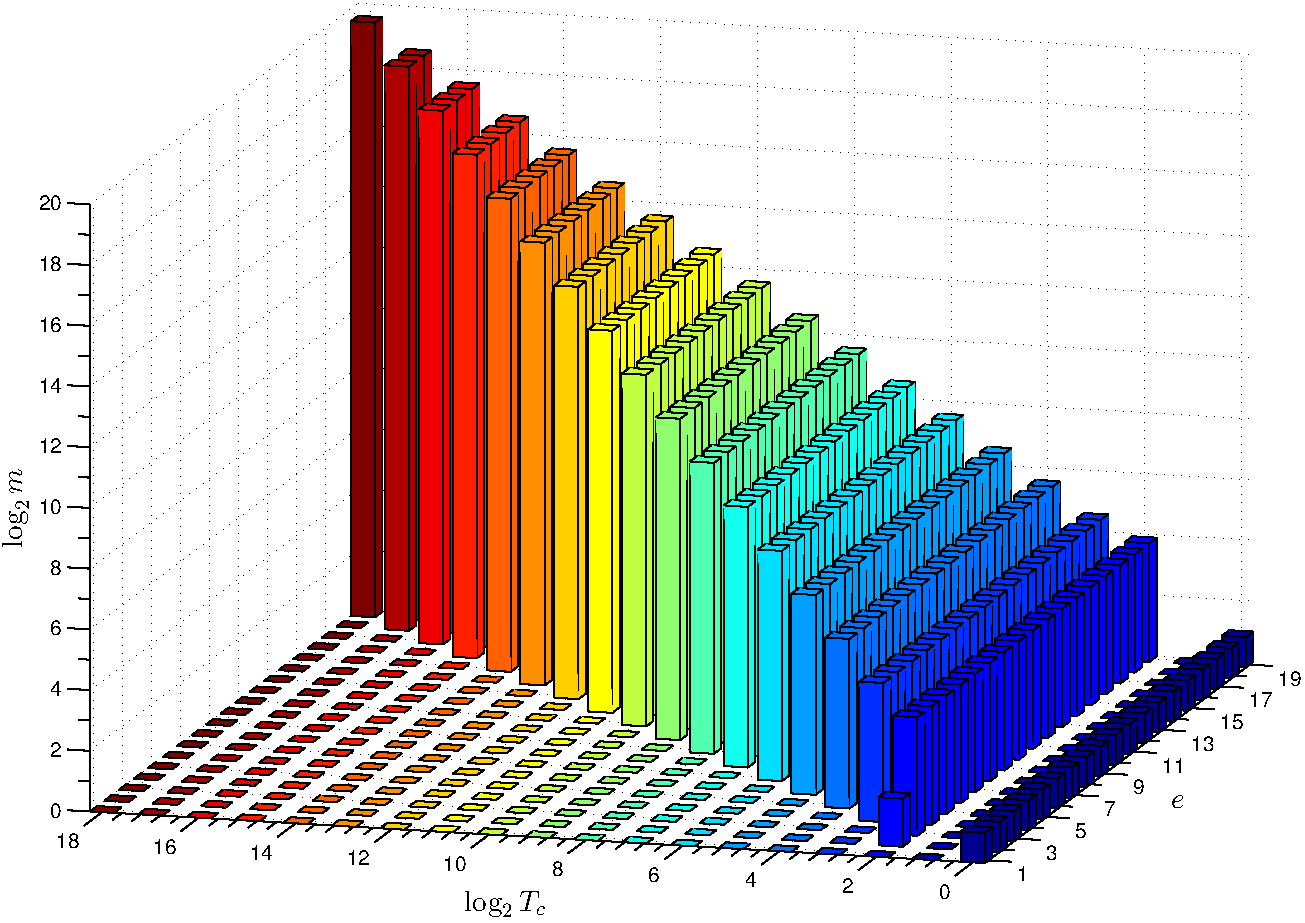
\includegraphics[width=0.95\BigOneImW]{e_T_m_3D_hist_a6b7}
b)
\end{minipage}\\
\begin{minipage}{0.95\BigOneImW}
\centering
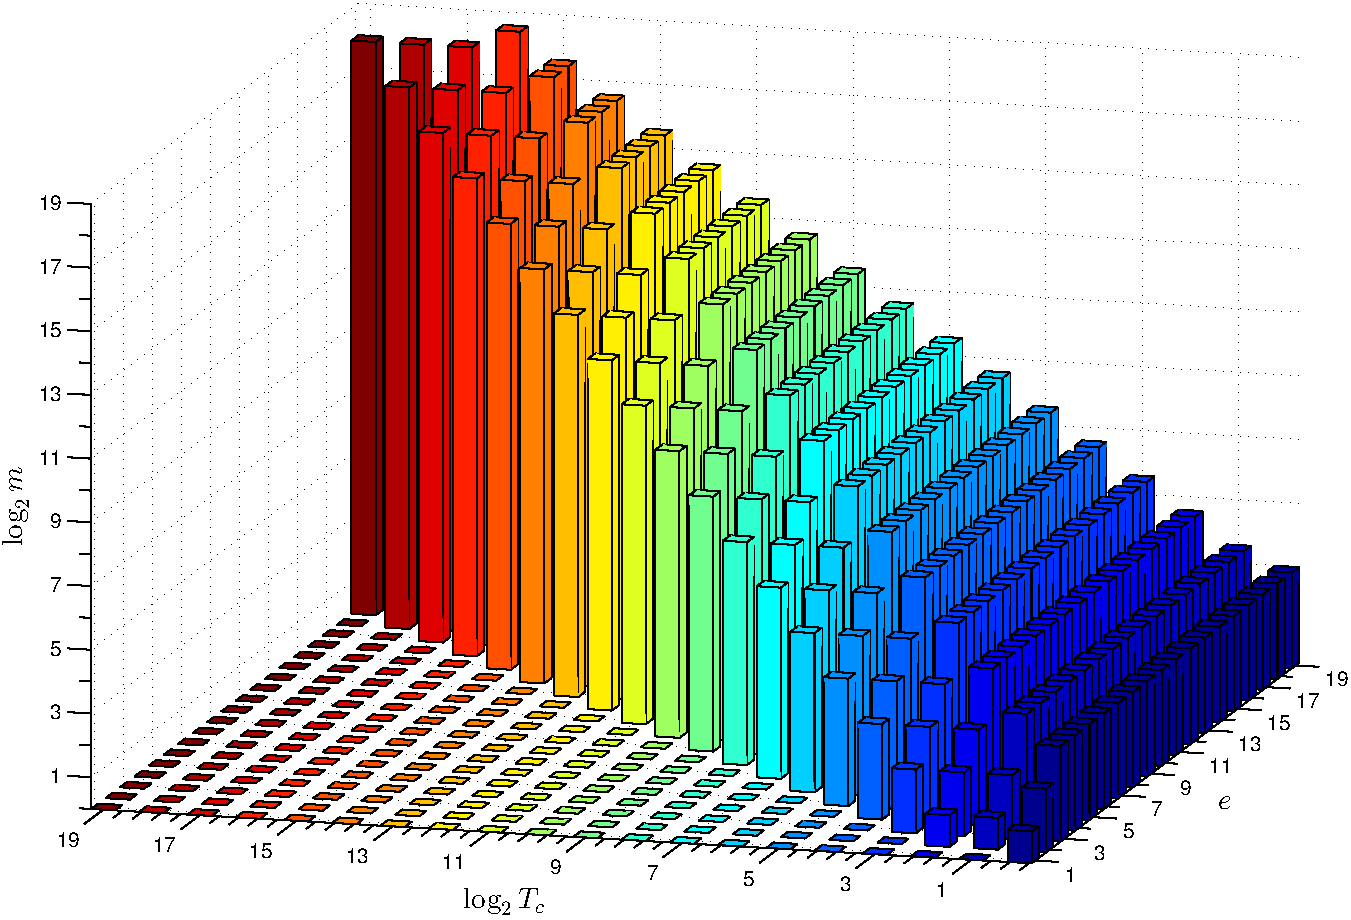
\includegraphics[width=0.95\BigOneImW]{e_T_m_3D_hist_a7b8}
c)
\end{minipage} \hspace{1mm}
\begin{minipage}{0.95\BigOneImW}
\centering
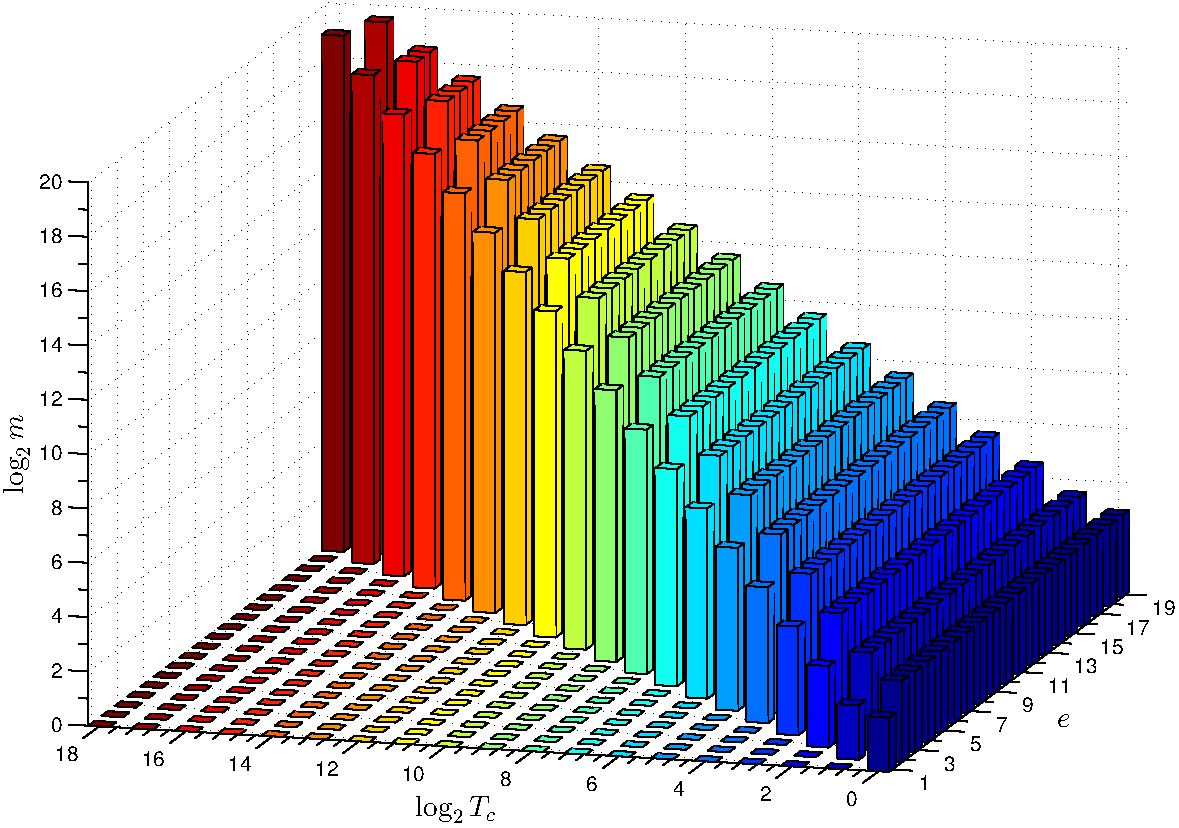
\includegraphics[width=0.95\BigOneImW]{e_T_m_3D_hist_a12b14}
d)
\end{minipage}
\caption{有限域$\mathbb{Z}_{2^e}$上GDCM~(\ref{eq:ArnoldInteger})的环分布,其中$e=1\sim 19$:
a) $(p, q)=(5, 7)$; b) $(p, q)=(6, 7)$; c) $(p, q)=(7, 8)$; b) $(p, q)=(12, 14)$}
\label{fig:perioddistributionc}
\end{figure*}

\begin{Property}
给定SMN\ $F_e$中环$\textbf{Z}_e=\{z_{n, e}\}_{n=0}^{T_c-1}=\{(x_{n, e}$, $y_{n, e})\}_{n=0}^{T_c-1}$及其上任意节点$z_{n_0, e}$,
SMN\ $F_{e+1}$中节点$z_{n_0, e+1}$所在环为
	\begin{equation*}
	\textbf{Z}_{e+1}=\left\{ z_{n, e+1} \right\}_{n=n_0}^{n_0+kT_c-1},
	\end{equation*}
	其中
	\begin{equation}
	k = \#\{(a_{n_0}, b_{n_0}), (a_{n_0+T_c}, b_{n_0+T_c}), (a_{n_0+2T_c}, b_{n_0+2T_c}), (a_{n_0+3T_c}, b_{n_0+3T_c})\},
	\label{numberElements}	
	\end{equation}
对任意$n\ge T_c$,$n'=n\bmod T_c$,存在$z_{n, e}=z_{n', e}$。
$\{(a_{n}, b_{n})\}_{n=n_0}^{n_0+3T_c}$由~\eqref{eq:kxky}式迭代生成,$\#(\cdot)$返回集合基数。
\label{Prop:cycleExpan}
\end{Property}

\begin{proof}
给定环$\textbf{Z}_e$上任意节点$z_{n_0, e}$和~(\ref{eq:kxky})式中向量$(k_x, k_y)$,则~(\ref{eq:kxky})式为集合上
$\{(0, 0), (0, 1), (1, 0), (1, 1) \}$的双射。
$z_{n, e+1}\in \{z_{j, e+1}\}_{j=n_0}^n$当且仅当$(n-n_0)\bmod T_c=0$,且$n>n_0$。\qedsymbol
\end{proof}

\begin{Property}
若SMN\ $F_e$中环$\textbf{Z}_e$和SMN\ $F_{e+1}中环$$\textbf{Z}^i_{e+1}$满足条件~(\ref{eq:condition}),则
\begin{equation}
	\begin{bmatrix}
		a^d_{n+1,e+1}\\
		b^d_{n+1,e+1}
	\end{bmatrix}
	=
	\begin{bmatrix}
		1 & p    \\
		q & 1+p\cdot q
	\end{bmatrix}\cdot
	\begin{bmatrix}
		a^d_{n,e+1}+a^d_{n,e}  \\
		b^d_{n,e+1}+b^d_{n,e}
	\end{bmatrix} \bmod 2,
		\label{anebne}
\end{equation}
其中$a^d_{n,e}, a^d_{n,e}\in \{-1, 0, 1\}$,$i=1\sim 2$。
\end{Property}
\begin{proof}
将~\eqref{eq:condition}式代入~\eqref{eq:k2xk2y}式,可得
\begin{equation}
	\begin{bmatrix}
		k'_x \\
		k'_y
	\end{bmatrix}
	=
	\begin{bmatrix}
		1 & p    \\
		q & 1+p\cdot q
	\end{bmatrix}\cdot
	\begin{bmatrix}
	x_{n,e}+a^i_{n,e}\cdot 2^e\\
    y_{n,e}+b^i_{n,e}\cdot 2^e
	\end{bmatrix},
\end{equation}
且$k^i_x=\lfloor k'_x/2^e\rfloor$,$k^i_y=\lfloor k'_y/2^e\rfloor$。

将上述计算结果代入~\eqref{eq:kxky}式,进一步可得
\begin{equation}
    \begin{bmatrix}
		a^1_{n+1, e+1}\\
		b^1_{n+1, e+1}
	\end{bmatrix}
     =
	\left[\begin{bmatrix}
		1 & p    \\
		q & 1+p\cdot q
	\end{bmatrix}
	\begin{bmatrix}
		a^1_{n, e+1}\\
		b^1_{n, e+1}
	\end{bmatrix}+
    \begin{bmatrix}
		k^1_x\\
		k^1_y
	\end{bmatrix}\right]
	\bmod 2,
	\label{eq:a1b1diff}
\end{equation}
\begin{equation}
    \begin{bmatrix}
		a^2_{n+1, e+1}\\
		b^2_{n+1, e+1}
	\end{bmatrix}
     =
	\left[\begin{bmatrix}
		1 & p    \\
		q & 1+p\cdot q
	\end{bmatrix}
	\begin{bmatrix}
		a^2_{n, e+1}\\
		b^2_{n, e+1}
	\end{bmatrix}+
    \begin{bmatrix}
		k^2_x\\
		k^2_y
	\end{bmatrix}\right]
	\bmod 2.
	\label{eq:a2b2diff}
\end{equation}
故将~\eqref{eq:a1b1diff}式与~\eqref{eq:a2b2diff}式相减即可证明上述性质。\qedsymbol
\end{proof}

\begin{table*}[!htb]
\caption{$p, q\in \mathbb{Z}_{17}$时满足猜想~\ref{Conjecture:eTc}的阈值$e_{s}, T_{s}$} % title of Table
\centering % used for centering table
\resizebox{\textwidth}{40mm}{
\begin{tabular}{*{16}{c|}c} % centered columns (4 columns)
\hline %inserts double horizontal lines
\diagbox[width=6em]{$p$}{$e, T_c$}{$q$}
&$1$&   $2$&   $3$&   $4$&   $5$&   $6$&   $7$&   $8$&   $9$&   $10$&   $11$&   $12$&   $13$&   $14$&   $15$&   $16$\\ \hline
1&	3,6&	4,8&	4,12&	2,4&	4,6&	5,8&	5,12&	1,2&	3,6&	4,8&	4,12&	2,4&	5,6&	6,8&	6,12&	1,2\\
2&	4,8&	3,4&	5,8&	2,2&	4,8&	3,4&	6,8&	2,2&	4,8&	3,4&	5,8&	2,2&	4,8&	3,4&	7,8&	2,2\\
3&	4,12&	5,8&	3,6&	2,4&	6,12&	4,8&	4,6&	1,2&	4,12&	7,8&	3,6&	2,4&	5,12&	4,8&	5,6&	1,2\\
4&	2,4&	2,2&	2,4&	3,2&	2,4&	2,2&	2,4&	3,2&	2,4&	2,2&	2,4&	3,2&	2,4&	2,2&	2,4&	3,2\\
5&	4,6&	4,8&	6,12&	2,4&	3,6&	7,8&	4,12&	1,2&	5,6&	4,8&	5,12&	2,4&	3,6&	5,8&	4,12&	1,2\\
6&	5,8&	3,4&	4,8&	2,2&	7,8&	3,4&	4,8&	2,2&	5,8&	3,4&	4,8&	2,2&	6,8&	3,4&	4,8&	2,2\\
7&	5,12&	6,8&	4,6&	2,4&	4,12&	4,8&	3,6&	1,2&	8,12&	5,8&	5,6&	2,4&	4,12&	4,8&	3,6&	1,2\\
8&	1,2&	2,2&	1,2&	3,2&	1,2&	2,2&	1,2&	4,2&	1,2&	2,2&	1,2&	3,2&	1,2&	2,2&	1,2&	4,2\\
9&	3,6&	4,8&	4,12&	2,4&	5,6&	5,8&	8,12&	1,2&	3,6&	4,8&	4,12&	2,4&	4,6&	9,8&	5,12&	1,2\\
10&	4,8&	3,4&	7,8&	2,2&	4,8&	3,4&	5,8&	2,2&	4,8&	3,4&	6,8&	2,2&	4,8&	3,4&	5,8&	2,2\\
11&	4,12&	5,8&	3,6&	2,4&	5,12&	4,8&	5,6&	1,2&	4,12&	6,8&	3,6&	2,4&	6,12&	4,8&	4,6&	1,2\\
12&	2,4&	2,2&	2,4&	3,2&	2,4&	2,2&	2,4&	3,2&	2,4&	2,2&	2,4&	3,2&	2,4&	2,2&	2,4&	3,2\\
13&	5,6&	4,8&	5,12&	2,4&	3,6&	6,8&	4,12&	1,2&	4,6&	4,8&	6,12&	2,4&	3,6&	5,8&	4,12&	1,2\\
14&	6,8&	3,4&	4,8&	2,2&	5,8&	3,4&	4,8&	2,2&	9,8&	3,4&	4,8&	2,2&	5,8&	3,4&	4,8&	2,2\\
15&	6,12&	7,8&	5,6&	2,4&	4,12&	4,8&	3,6&	1,2&	5,12&	5,8&	4,6&	2,4&	4,12&	4,8&	3,6&	1,2\\
16&	1,2&	2,2&	1,2&	3,2&	1,2&	2,2&	1,2&	4,2&	1,2&	2,2&	1,2&	3,2&	1,2&	2,2&	1,2&	5,2\\
\hline %inserts single line
\end{tabular}}
\label{table:num} % is used to refer this table in the text
\end{table*}


SMN\ $F_e$中周期为$T_c$的环演化结果对应SMN\ $F_{e+1}$中以下5种可能情况:
1) 4个周期为$T_c$的环; 2) 1个周期为$2T_c$的环和2个周期为$T_c$的环; 3) 2个周期为$2T_c$的环;
4) 1个周期为$3T_c$的环和1个周期为$T_c$的环; 5) 1个周期为$4T_c$的环。
举例来说,图~\ref{fig:SMNcat} a)中自环$``0\rightarrow 0"$被演化为图~\ref{fig:SMNcat} b)中
自环$``0\rightarrow 0"$和环``$(0+2^1)=2\rightarrow (0+2^3)=8\rightarrow (0+2^1+2^3)=10\rightarrow 2$"。类似的,
图~\ref{fig:SMNcat} a)中环$``1\rightarrow 3\rightarrow 2\rightarrow 1"$被演化为图~\ref{fig:SMNcat} b)中
环``$1 \rightarrow (3+2^1+2^3)=13 \rightarrow (2+2^3+2)=12 \rightarrow (1+2^1)=3 \rightarrow (3+2^1+2)=7
\rightarrow (2+2^1)=4 \rightarrow 1$"和
环``$(1+2^3)=9\rightarrow (3+2^1+2^3+2)=15 \rightarrow (2+2^1+2)=6 \rightarrow (1+2^1+2^3)=11 \rightarrow (3+2^1)=5
\rightarrow (2+2^1+2^3+2)=14 \rightarrow 9$"。
根据上述分析可知,$e\ge 3$时GDCM~(\ref{eq:ArnoldInteger})状态映射网络是由$e=1$其状态映射网络演化而来的,
例如SMN\ $F_e$中周期为3的倍数的环由SMN\ $F_1$中周期为3的基环生成。
图~\ref{Functionalgraphse1}第6个子图中自环$``8\rightarrow 8"$被扩展为图~\ref{fig:Figure3d3c}中环
$``16\rightarrow 52 \rightarrow 48 \rightarrow 20 \rightarrow 16"$,
图~\ref{Functionalgraphse1}第9个子图中自环$``2\rightarrow 2"$被扩展为图~\ref{fig:Figure3d3c}中环
$``2\rightarrow 34 \rightarrow 6 \rightarrow 38 \rightarrow 2"$。
注意到,图~\ref{fig:perioddistributione1} c)中环$``1\rightarrow 1"$被扩展为图~\ref{Functionalgraphse1}中第9个子图中环
$``1\rightarrow 9 \rightarrow 3 \rightarrow 11 \rightarrow 1"$,图~\ref{fig:perioddistributione1} c)中环$``0\rightarrow 0"$
被扩展为对应状态映射网络中3个环:
$``0\rightarrow 0"$,$``2\rightarrow 2"$,$``8\rightarrow 10\rightarrow 8"$。
此外,图~\ref{fig:SMNcat} b)中环$``1\rightarrow 13 \rightarrow 12 \rightarrow 3 \rightarrow 7 \rightarrow 4 \rightarrow 1"$
被扩展为~\ref{fig:SMNcat} c)左下侧所示周期相同的4个环。
因此上述5种可能情况均可在图~\ref{fig:SMNcat}、\ref{fig:perioddistributione1}、\ref{Functionalgraphse1}中被发现。

根据图~\ref{fig:perioddistributionab}可以看出,SMN\ $F_e$中环的周期分布呈幂律分布,图~\ref{fig:perioddistributionc}为其3维柱状图,其中
$T_c$表示SMN\ $F_e$中环的周期。

\begin{Conjecture}
存在阈值$e_{s}$和$T_{s}$,使得SMN\ $F_e$中周期为$T_c$的环数与SMN\ $F_{e+1}$中周期为$2T_c$的环数满足关系
\begin{equation}
  2 N_{T_c, e}=
  \left.\begin{cases}
  N_{2T_c, e+1}       & T_c\ge T_{s};\\
  2 N_{T_c, e_s}      & T_c<T_{s},
  \end{cases}\right.
  \label{thresholdCondition}
\end{equation}
这里$e\ge e_{s}$。
\label{Conjecture:eTc}
\end{Conjecture}

\begin{table}[!htb]
\caption{$(p, q)=(9, 14)$时SMN\ $F_e$中周期为$T_c$的环数} % title of Table
\centering % used for centering table
\begin{tabular}{*{8}{c|}c} % centered columns (4 columns)
\hline %inserts double horizontal lines
\diagbox[width=6em]{$e$}{$N_{T_c, e}$}{$T_c$}
&$2^0$ & $2^1$ &     $2^2$&     $2^3$&    $2^4$ &    $2^5$ &     $2^6$&    $2^7$ \\ \hline
1 &2 &1&     0&     0&     0&     0&      0&      0  \\
2 &2 &1&     3&     0&     0&     0&      0&      0  \\
3 &2 &1&    15&     0&     0&     0&      0&      0  \\
4 &2 &1&    63&     0&     0&     0&      0&      0  \\
5 &2 &1&   255&     0&     0&     0&      0&      0  \\
6 &2 &1&  1023&     0&     0&     0&      0&      0  \\
7 &2 &1&  4095&     0&     0&     0&      0&      0  \\
8 &2 &1& 16383&     0&     0&     0&      0&      0  \\
9 &2 &1& 16383& 24576&     0&     0&      0&      0  \\ \hdashline
10&2 &1& 16383& 24576& 49152&     0&      0&      0  \\
11&2 &1& 16383& 24576& 49152& 98304&      0&      0  \\
12&2 &1& 16383& 24576& 49152& 98304& 196608&      0  \\
13&2 &1& 16383& 24576& 49152& 98304& 196608& 393216  \\\hline %inserts single line
\end{tabular}
\label{table:pqeTc} % is used to refer this table in the text
\end{table}

根据性质~\ref{Prop:cycleExpan}可知,SMN\ $F_e$中环$\textbf{Z}_e$由$F_1$中对应基环逐渐扩展而来,
因此SMN\ $F_{e+1}$中给定周期的环数与SMN\ $F_{e}$中对应周期的环数满足某种线性关系,其与参数$p, q$有关。
这里将其归结为猜想~\ref{Conjecture:eTc},该猜想可以通过$(p, q)$上的大量随机实验进一步得到验证,
表~\ref{table:num}给出$p, q\in \mathbb{Z}_{17}$时满足猜想~\ref{Conjecture:eTc}的$e_{s}, T_{s}$。
根据表~\ref{table:num},阈值$e_{s}, T_{s}$相对较小,$\mathit{Prob}[e_{s}\le \log_2(16)=4]=25/32$。
从图~\ref{fig:perioddistributionab}可以看出,
等式~(\ref{thresholdCondition})中第一种情况表示当$e$足够大时SMN\ $F_e$中环的周期分布呈指数为1的幂律分布,
当$e\ge e_{s}$时SMN\ $F_{e+1}$中任意周期的环数可以依据SMN\ $F_{e}$中对应周期的环数推导出来,
此外,根据图~\ref{fig:perioddistributionc},
等式~(\ref{thresholdCondition})中第二种情况表示任意周期的环数关于$e$单调增加,趋于常数。
表~\ref{table:pqeTc}给出$(p, q)=(9, 14)$时SMN\ $F_e$中周期为$T_c$的环量,可进一步验证上述分析讨论。

\section{关于离散Cat映射UPO's的讨论}

混沌系统中不稳定周期轨道(UPO's)的识别一直都是周期轨道理论的研究热点,
构成混沌吸引子基本架构的无穷多不稳定周期轨道(UPO's)的稳定性取决于其与相空间中相邻轨道距离的变化趋势\upcite{Davidchack1999PRE}。
\iffalse
周期轨道理论认为,混沌动力学系统在相空间中生成的混沌吸引子包含了无穷多的不稳定周期轨道(UPO's)\upcite{Davidchack1999PRE},
它们构成了混沌吸引子的骨架,其稳定性取决于其与相空间中相邻轨道的距离变化趋势。\fi
在\upcite{Catchen2013period2e}中摘要部分,F. Chen等人认为其研究有助于识别原始Cat映射的不稳定周期轨道,
但其与通过分析GDCM~(\ref{eq:ArnoldInteger})内部结构的演化过程所得结论不一致。
图~\ref{fig:upo}为图~\ref{fig:SMNcat} c)中环的相对位置,结合图~\ref{fig:SMNcat}和图~\ref{fig:upo}可以发现,
拥有指定周期的Cat映射的数量与对应状态映射网络中环的数量和相邻环之间的距离没有任何关系,
因此依据指定周期的Cat映射的数量无法识别嵌入在混沌吸引子中的不稳定周期轨道(UPO's)。

\begin{figure}[!htb]
	\centering
	\begin{minipage}{1.25\BigOneImW}
		\centering
		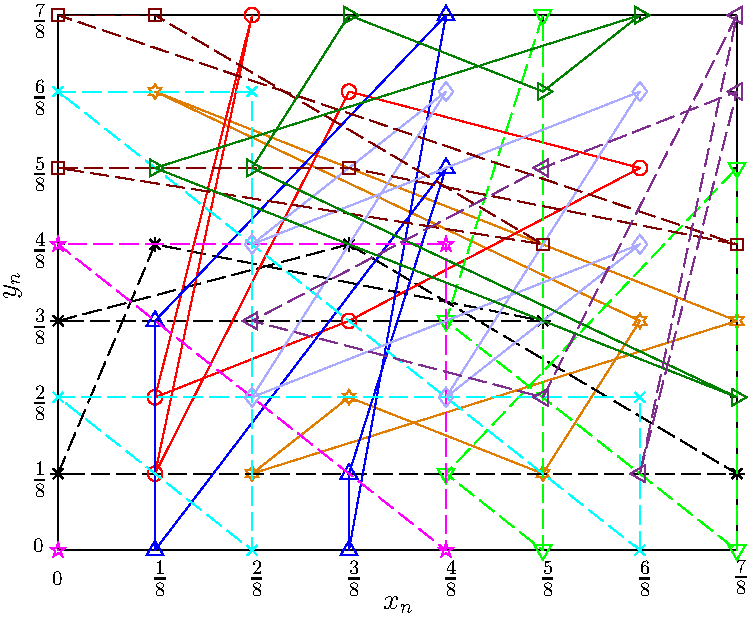
\includegraphics[width=1.25\BigOneImW]{UPO}		
	\end{minipage}
\caption{$N={2^3}, (p, q)=(1, 3)$时GDCM~(\ref{eq:ArnoldInteger})的二维图形表示}
\label{fig:upo}
\end{figure}

\section{本章小结}

本章讨论了定点运算域上离散Cat映射的动力学特性,厘清了有限域上周期为$T$的不同离散Cat映射的数量$N_T$与周期$T$之间的关系,
揭示了定点运算域上离散Cat映射的状态映射网络$F_e$与$F_{e+1}$之间的关系,即状态映射网络与实现精度之间的关系,
研究发现,离散Cat映射状态网络中环的分布呈指数为1的幂律分布,但其幂律分布仍需进一步理论证明。